\chapter{Optymalizacja konstrukcji na przykładzie wiaduktu w ciągu Pomorskiej Kolei Metropolitalnej}

\textit{Streszczenie: W niniejszym rozdziale opisano pełny proces optymalizacji kolejowego wiaduktu łukowego z uwzględnieniem oddziaływań dynamicznych kolei dużych prędkości. Analizę przeprowadzono na przykładzie istniejącego wiaduktu WK2 w ciągu Pomorskiej Kolei Metropolitalnej. W pierwszej kolejności podano charakterystykę wiaduktu oraz opisano stworzony model numeryczny MES wiaduktu. Następnie przedstawiono przeprowadzony eksperyment oraz identyfikację modalną za pomocą metody NExT-ERA istniejącego obiektu. Wyznaczone parametry posłużyły do kalibracji modelu za pomocą aplikacji korzystającej z optymalizacji PSO. Na wykonanym modelu, dla różnych wariantów konstrukcji oraz prędkości maksymalnych przejazdu wykonano szereg obliczeń optymalizacyjnych. Rezultaty optymalizacji zebrano i poddano analizie statystycznej oraz przedstawiono w formie graficznej. Na koniec sformułowano wnioski dotyczące najistotniejszych elementów konstrukcyjnych wpływających na organicznie drgań w kolejowych mostach łukowych.}


\section{Charakterystyka obiektu}
Obiekt badawczy stanowi kolejowy wiadukt łukowy w ciągu linii Pomorskiej Kolei Metropolitalnej w km 1+696,02 \parencite{Filipiuk2015,TransprojektGdanski2014}. Przęsło wiaduktu stanowi stalowy ustój łukowy z jazdą dołem. Widok z boku na konstrukcję stalową wiaduktu pokazano na rysunkach \ref{fig: wk2_side_view}. Główne wymiary charakteryzujące konstrukcję są następujące: 
\begin{itemize}[noitemsep]
	\item rozpiętość teoretyczna: $L_t=70.00 \text{m}$, 
	\item długość całkowita:  $L_c=71,60 \text{m}$, 
	\item wysokość w kluczu:  $H=11.00 \text{m}$,
	\item rozstaw osiowy dźwigarów: $B_t = 7.35 \text{m}$,
	\item szerokość całkowita: $B_c=10.21 \text{m}$. 
\end{itemize}
 \begin{figure}[hbt!]
	\centering
	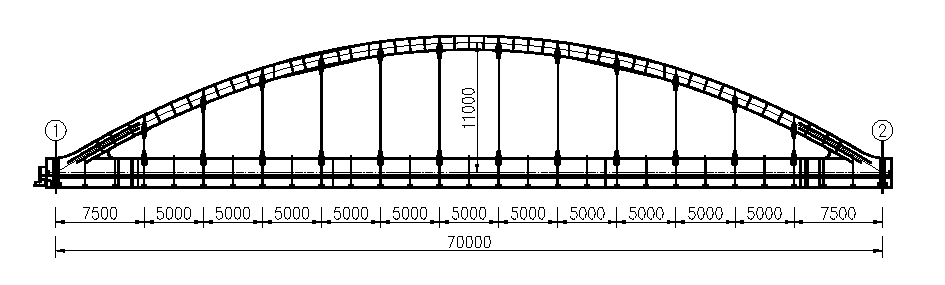
\includegraphics[trim=15 10 20 15, clip]{/WK2/rysunki/widok_z_boku_croped.pdf}
	\captionsetup{justification=centering}
	\caption{Widok z boku na konstrukcję stalową dźwigara łukowego wiaduktu WK3}
	\label{fig: wk2_side_view}
\end{figure}

 Przekrój poprzeczny dźwigarów łukowych zaprojektowano jako skrzynkowy (Rys. \ref{fig: wk2_cross_sect}). Pomost wykonano jako ortotropowy, z blachy wzmocnionej żebrami podłużnymi i poprzecznicami o przekroju teowym. Poprzecznice rozmieszczono w rozstawie 2.5 m. Ściąg łuku stanowią belki dwuteowe, po jednej dla każdego dźwigara łukowego. Przekrój ściągu zmienia się z dwuteowego na skrzynkowy w strefie podporowej. Na rysunku \ref{fig: wk2_cross_sect_deck} przestawiono przekrój poprzeczny pomostu i ściągu w strefie podporowej. 
  \begin{figure}[hbt!]
 	\centering
 	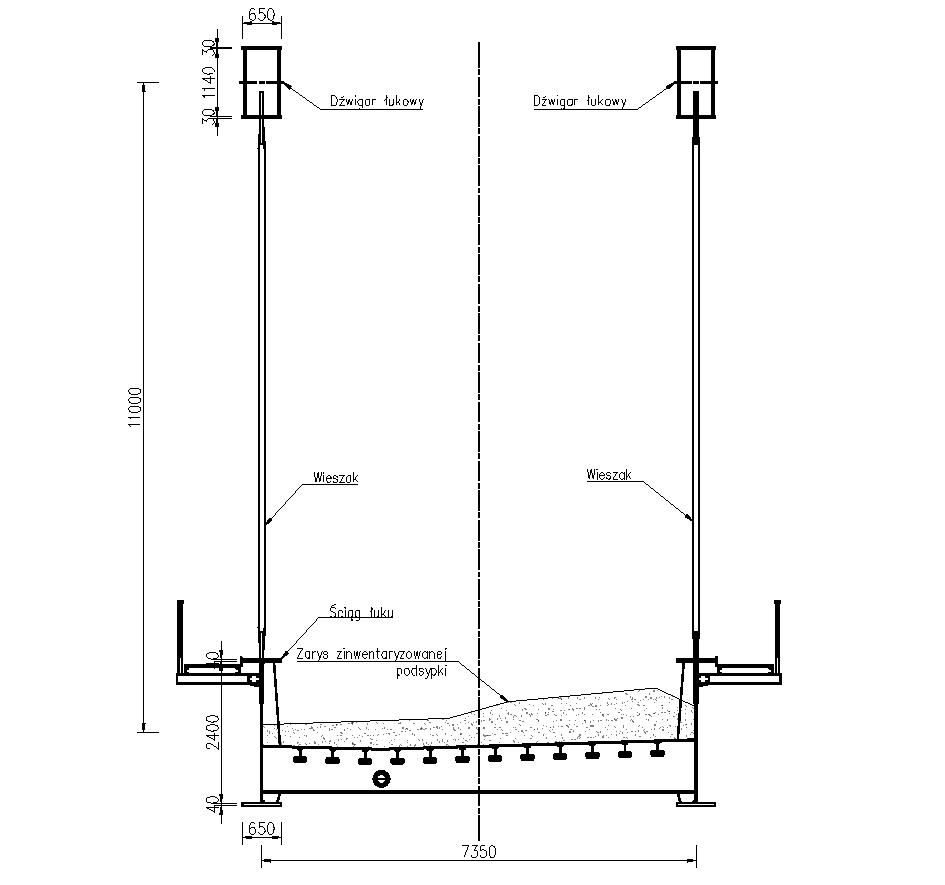
\includegraphics[]{/WK2/rysunki/przekroj_dzwigara_croped.pdf}
 	\captionsetup{justification=centering}
 	\caption{Przekrój poprzeczny konstrukcji stalowej wiaduktu WK2 w środku rozpiętości}
 	\label{fig: wk2_cross_sect}
 \end{figure}
 \begin{figure}[h]
 	\centering
 	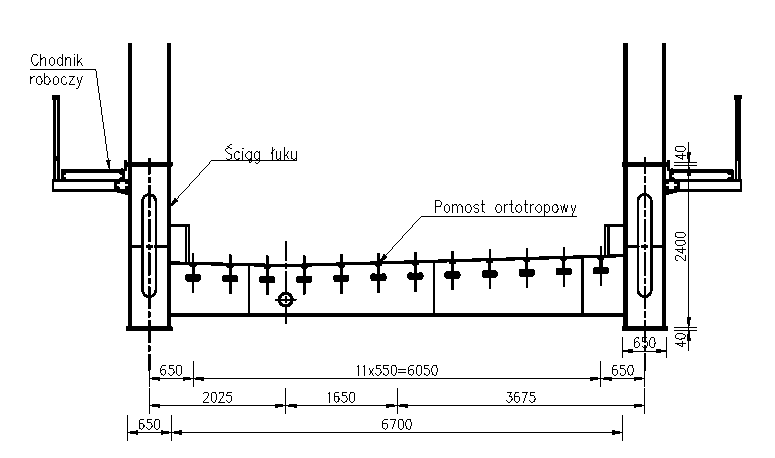
\includegraphics[]{/WK2/rysunki/przekroj_poprzeczny_croped.pdf}
 	\captionsetup{justification=centering}
 	\caption{Przekrój poprzeczny przez pomost w strefie podporowej wiaduktu WK2}
 	\label{fig: wk2_cross_sect_deck}
 \end{figure}
 
 W zrealizowanym wariancie pomost został podwieszony do łuku za pomocą prętowych, prostych wieszaków o średnicy 100 mm. Po każdej ze stron zamontowano 12 wieszaków w rozstawie co 5 m. Wieszaki zostały połączone z dźwigarem i ściągiem sztywnym połączeniem spawanym. Rzeczywisty widok zrealizowanego przęsła pokazano na rysunku \ref{fig: wk2_foto_widok_front}, detale konstrukcyjne w obrębie strefy podporowej na rysunku \ref{fig:  wk2_foto_wezglowie}, a połączenie wieszaka ze ściągiem na rysunku \ref{fig: wk2_foto_wieszak}.

\begin{figure}[hbt!]
	\centering
	\subfloat{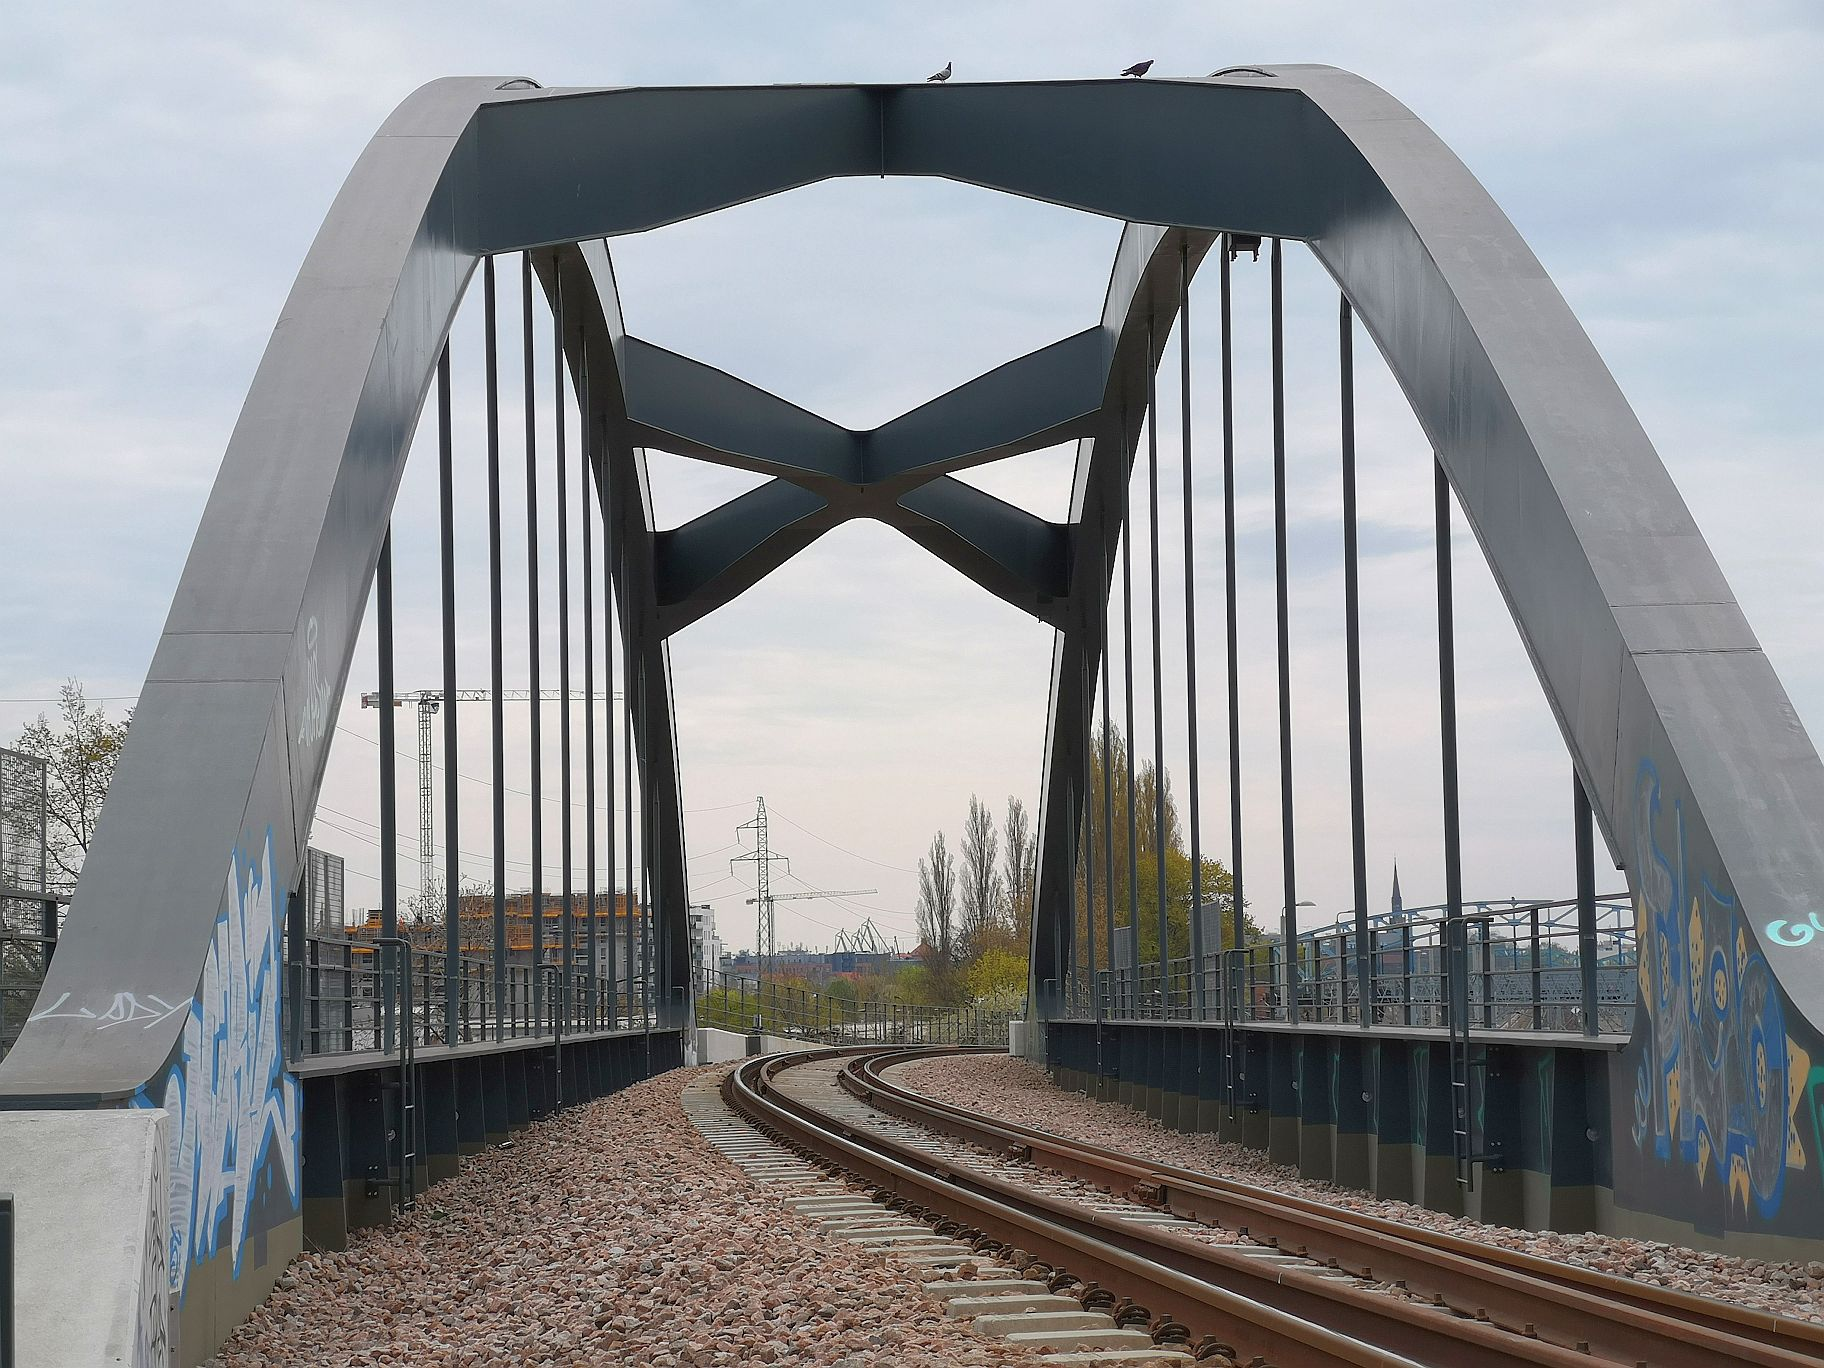
\includegraphics[height=0.30\textheight]{/WK2/zdjecia/widok_front2.jpg}} 
	\captionsetup{justification=centering}
	\caption{Widok od strony lotniska na wiadukt WK2 (arch. własne)}
	\label{fig: wk2_foto_widok_front}
\end{figure}
\begin{figure}[hbt!]
	\centering
	\subfloat[Widok z góry]{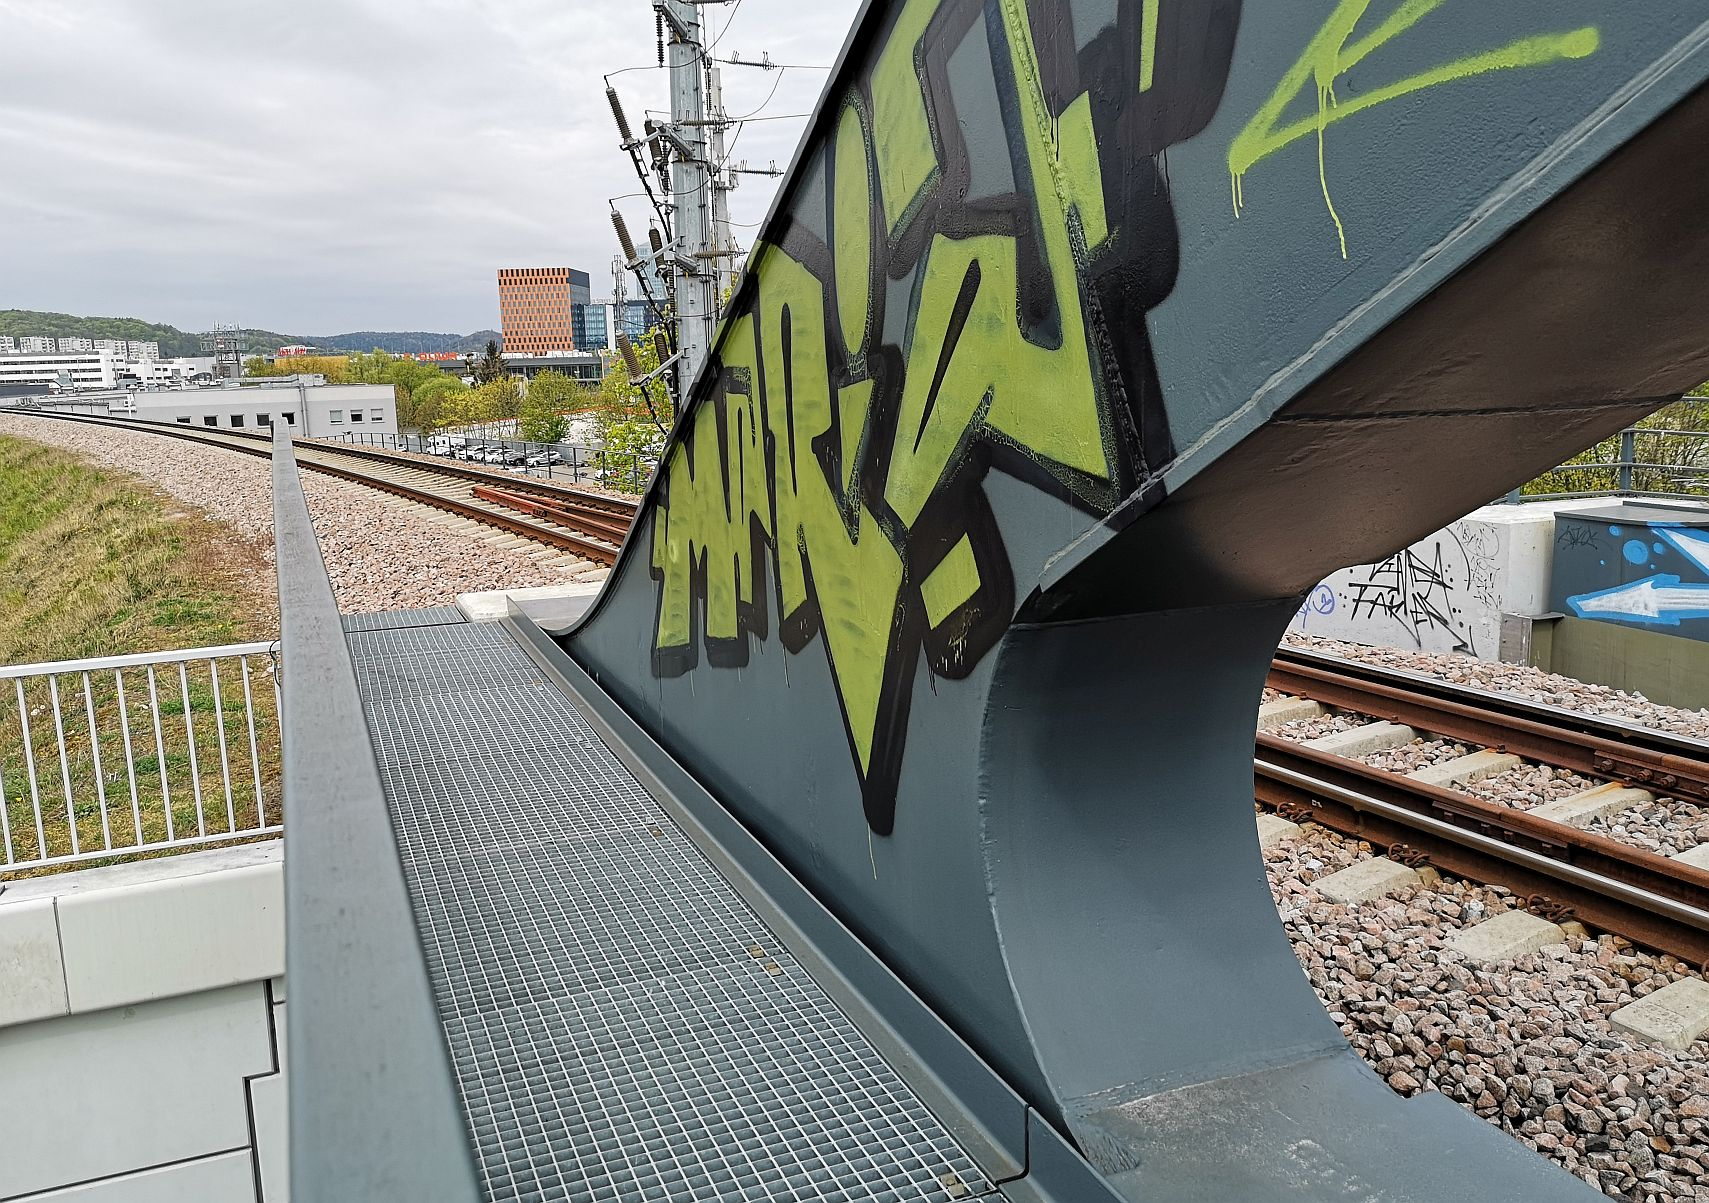
\includegraphics[height=0.2\textheight]{/WK2/zdjecia/wezglowie.jpg}} 
	\qquad
	\subfloat[Widok z dołu]{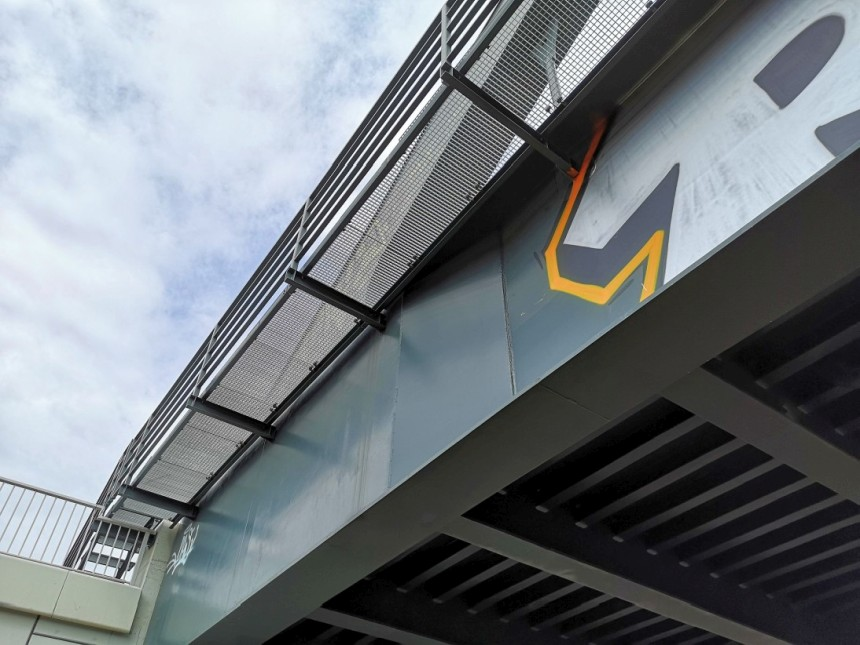
\includegraphics[height=0.2\textheight]{/WK2/zdjecia/detal_wezglowie_dol.jpg}}
	\captionsetup{justification=centering}
	\caption{Szczegóły konstrukcyjne w obrębie połączenia łuku ze ściągiem (arch. własne)}
	\label{fig: wk2_foto_wezglowie}
\end{figure}
\begin{figure}[hbt!]
	\centering
	\subfloat{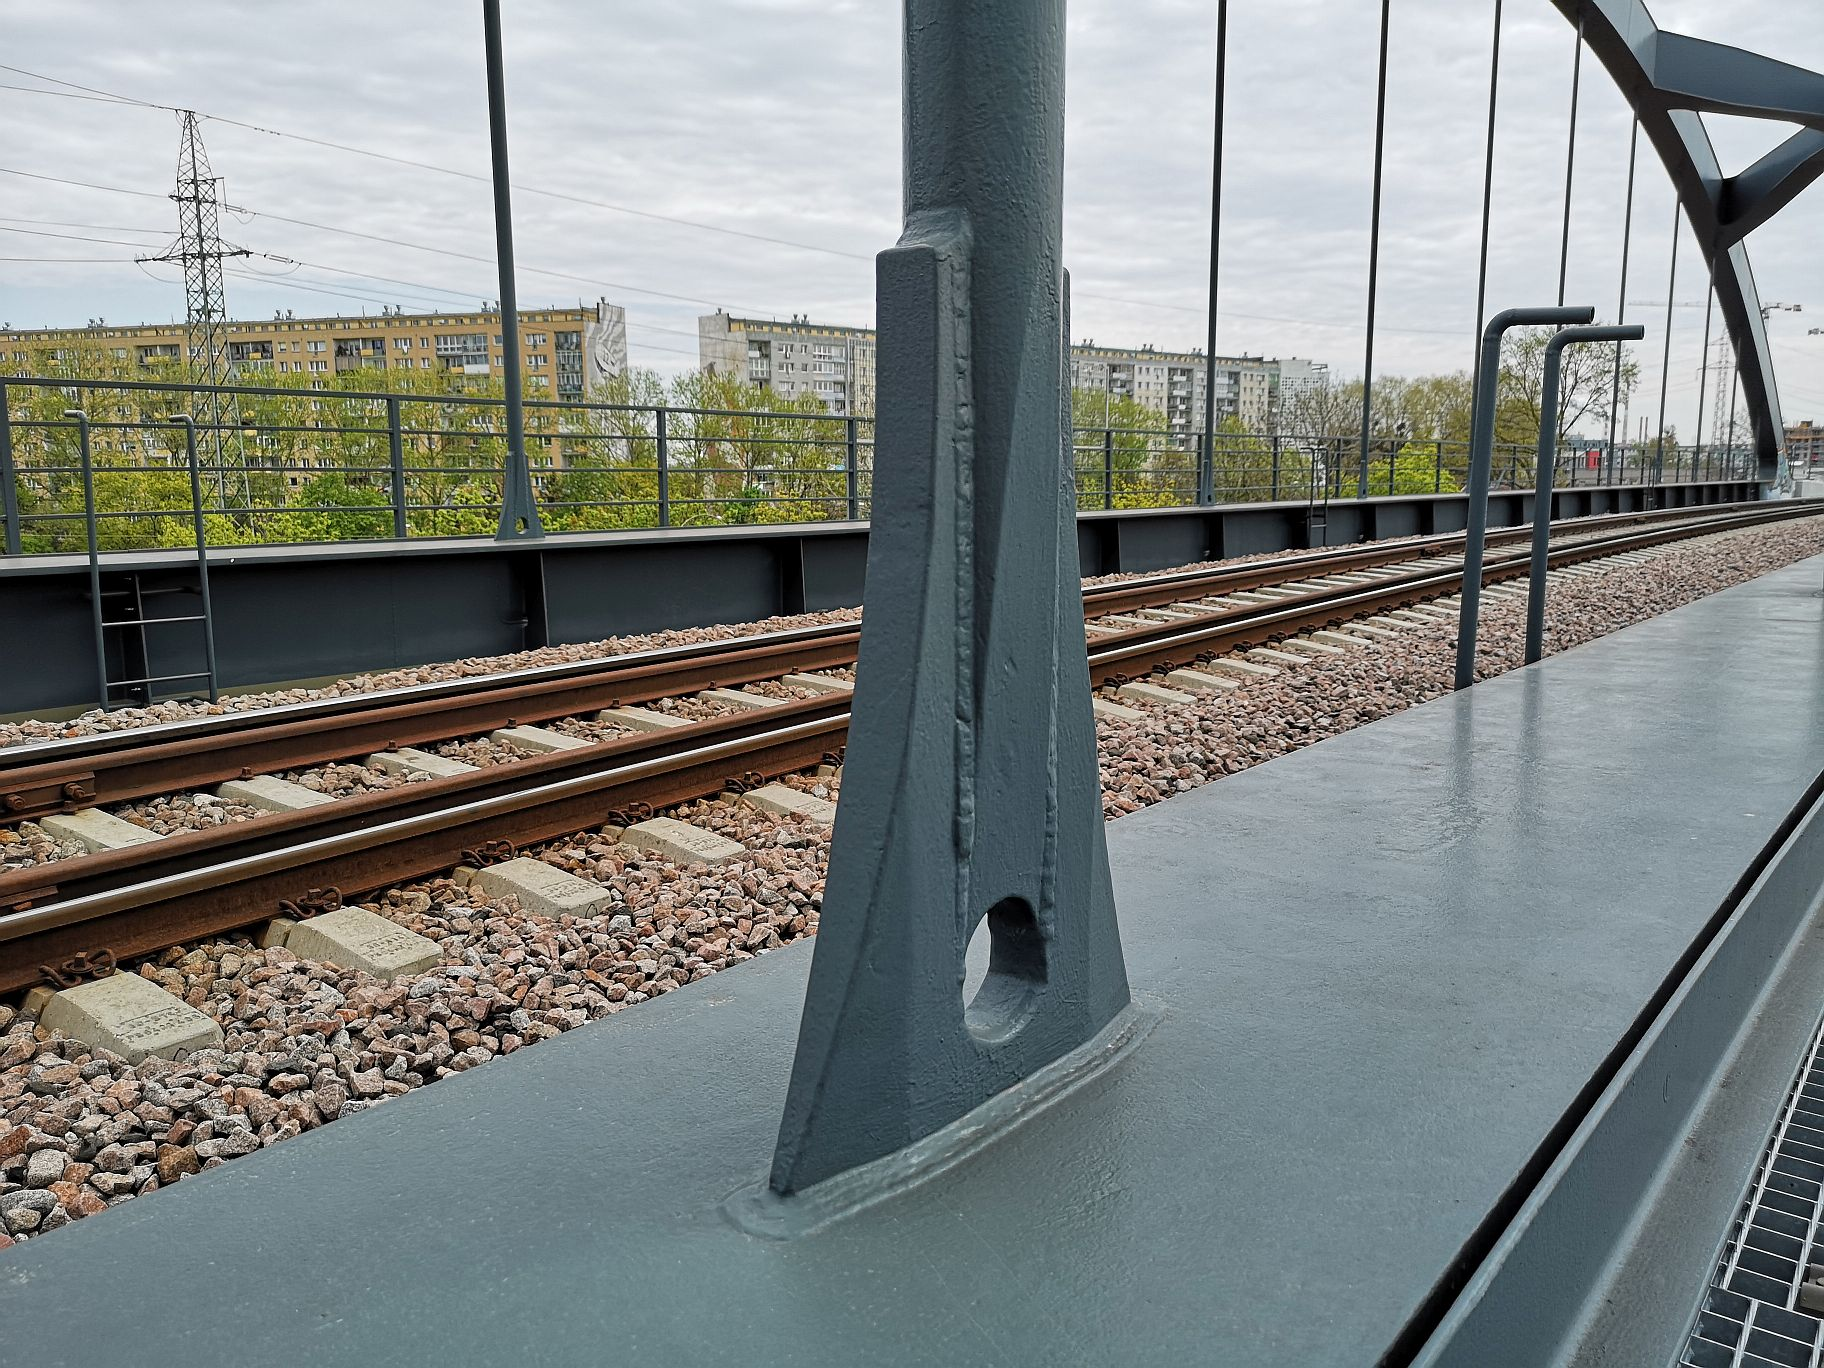
\includegraphics[height=0.2\textheight]{/WK2/zdjecia/zakotwienie_wieszak.jpg}}
	\captionsetup{justification=centering}
	\caption{Detal połączenia wieszaka łuku ze ściągiem (arch. własne)}
	\label{fig: wk2_foto_wieszak}
\end{figure}
Na obiekcie po wybudowaniu przeprowadzono badania odbiorcze. Próbne obciążenia odbyły się w dniu 14.04.2015 i zostały przeprowadzone przez zespół naukowców z Politechniki Śląskiej i Politechniki Gdańskiej \parencite{azinski2015}. Wykonano badania statyczne i dynamiczne. W ramach pomiarów statycznych zrealizowano dwa interesujące, z punktu widzenia tej pracy, ustawienia obciążenia. Ustawienie U1 z obciążeniem zorientowanym symetrycznie na obiekcie oraz ustawienie U2 z obciążeniem wywołującym maksymalne ugięcia w $1/4$ rozpiętości przęsła. Pomiary przemieszczeń wykonywano w 6 punktach zlokalizowanych w $1/4$, $1/2$ i $3/4$ rozpiętości przęsła, po obu jego stronach. Czujniki zamocowano do konstrukcji w osiach ściągów, na dolnych lub górnych pasach. Obciążenie statyczne stanowiły dwie lokomotywy spalinowe typu: SM-48 i BR232. Pomierzone ugięcia statyczne zostaną użyte jako dodatkowe kyterium kalibracji modelu numerycznego.
W ramach badań dynamicznych mierzono przyspieszenia konstrukcji po wymuszeniu obciążeniem impulsowym. Impuls generowano przez upadek jednej osi koparki dwudrogowej i zeskoków drezyny z progu. Na postawie przebiegów drgań swobodnych zidentyfikowano częstotliwości drgań własnych przęsła i towarzyszące im tłumienia. Do identyfikacji użyto algorytmu ERA. Zidentyfikowane częstotliwości drgań i tłumienia przęsła posłużą do porównania z wynikami badań przeprowadzonymi w ramach tej pracy.


\section{Budowa modelu numerycznego} \label{sect:wk2_basic_num_model}

Na potrzeby analiz numerycznych zbudowano model MES w środowisku SOFiSTiK (Rys. \ref{fig: model_wk2_visualization}) Model przestrzenny składa się kilku rodzajów elementów skończonych. Z jednowymiarowych elementów belkowych wykonano łuki, stężenia, belki ściągu, wzmocnienia wezgłowii i żebra pomostu ortotropowego. Elementami kratowymi odwzorowano wieszaki. Blachę pomostu wykonano z czterowęzłowych elementów powłokowych \parencite{SOFiSTiK2018}. Połączenia pomiędzy końcami wieszaków i osiami elementów łuku oraz ściągu zrealizowano przez połączenia kinematyczne translacji i rotacji węzłów. Podparcia pionowe w miejscach łożysk mostu zrealizowano za pomocą sztywnych więzów węzłów. Należy zwrócić uwagę, że nie zablokowano przesuwów podłużnych i poprzecznych za pomocą blokady przemieszczeń. Zamiast tego na obu kierunkach zamocowano elastyczne elementy (sprężyny) o wstępnie dobranej sztywności. Dla projektowo zablokowanych translacji elementom nadano bardzo dużą sztywność, a dla wolnych stopni swobody bardzo małą. Usztywnienia wezgłowii zamodelowano za pomocą rusztu elementów belkowych o przekroju składającym się z dwóch blach odsuniętych od siebie na szerokość przekroju skrzynkowego łuku. Elementy strukturalne konstrukcji (takie jak ściągi, pomost, dźwigary łukowe, elementy podparcia itd.) podzielono w modelu na grupy pozwalające odnosić się do nich jako całości. Przekroje elementów belkowych przyjęto zgodnie z dostępną dokumentacją \parencite{SOFiSTiK2018}. Wymiary przekrojów zmiennych po długości zostały interpolowane liniowo. Widoczne na rysunku \ref{fig: model_wk2_static_scheme} dodatkowe połączenia kinematyczne są przygotowaniem dla możliwości podłączenia innych konfiguracji wieszaków.



\begin{figure}[hbt!]
	\centering
	\subfloat[Widok A]{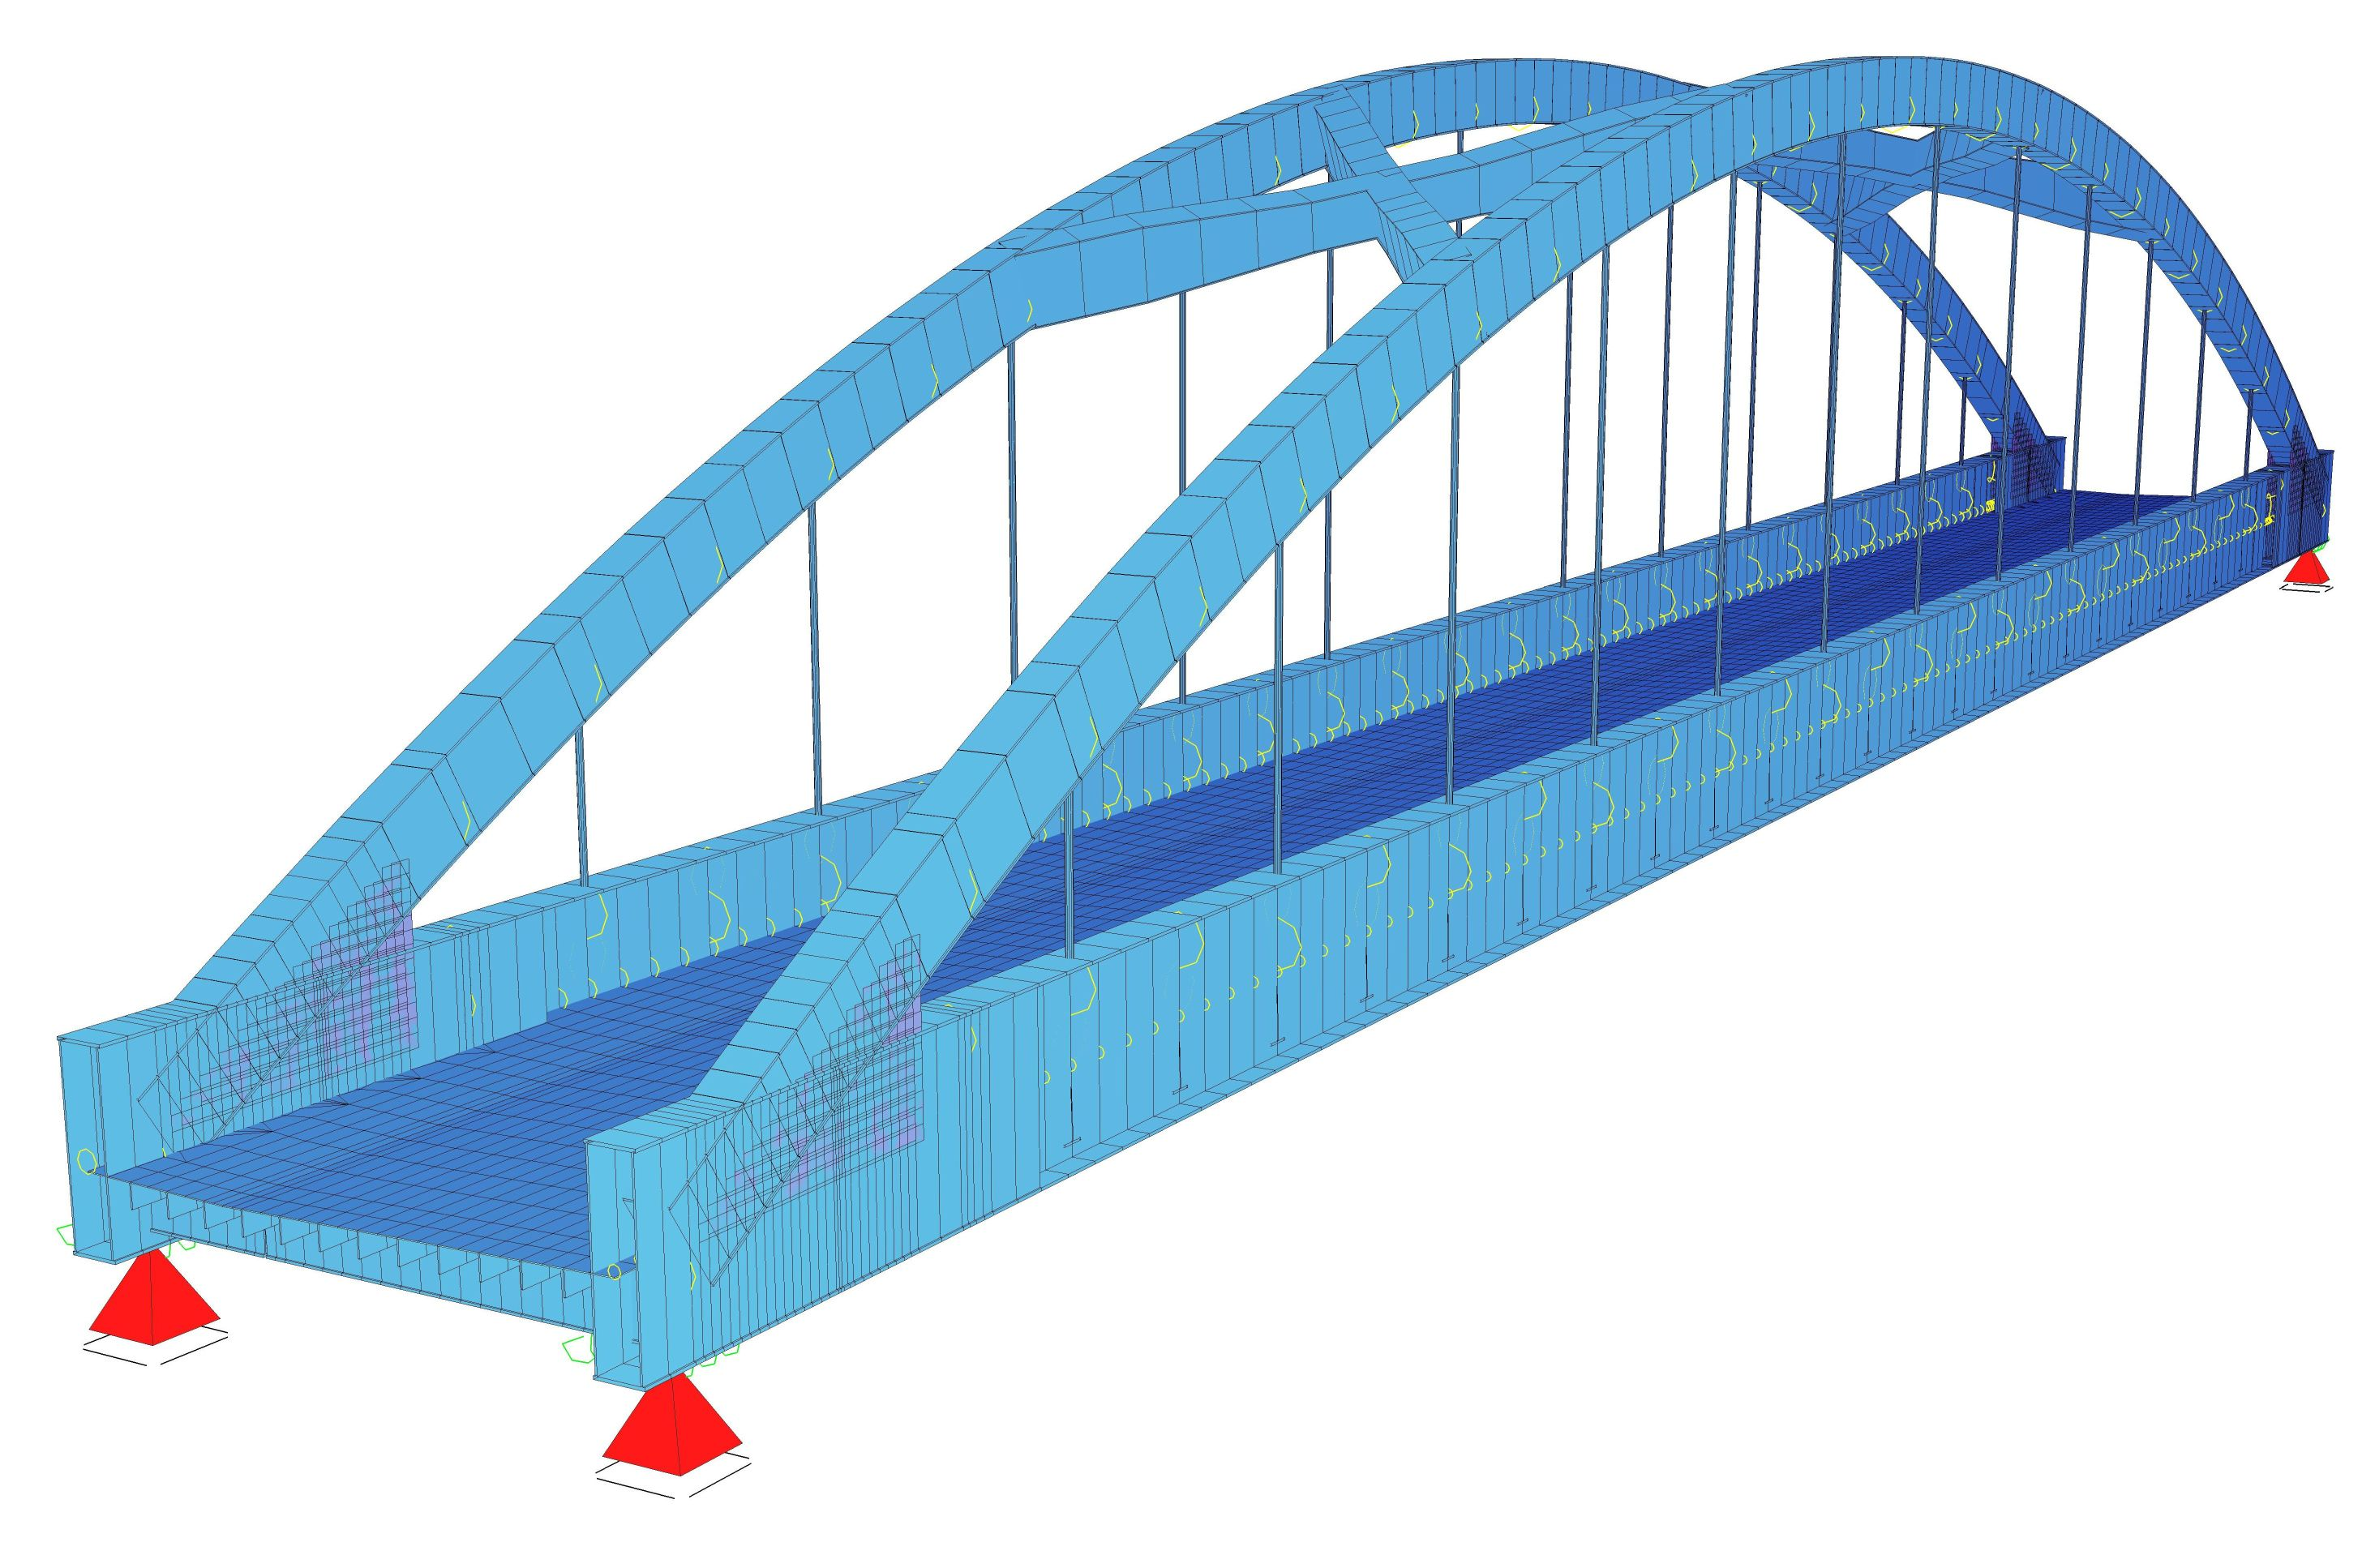
\includegraphics[width=0.5\linewidth]{/WK2/model/SCIAG_PAR_v01_vis_1.jpg}}%
	\subfloat[Widok B]{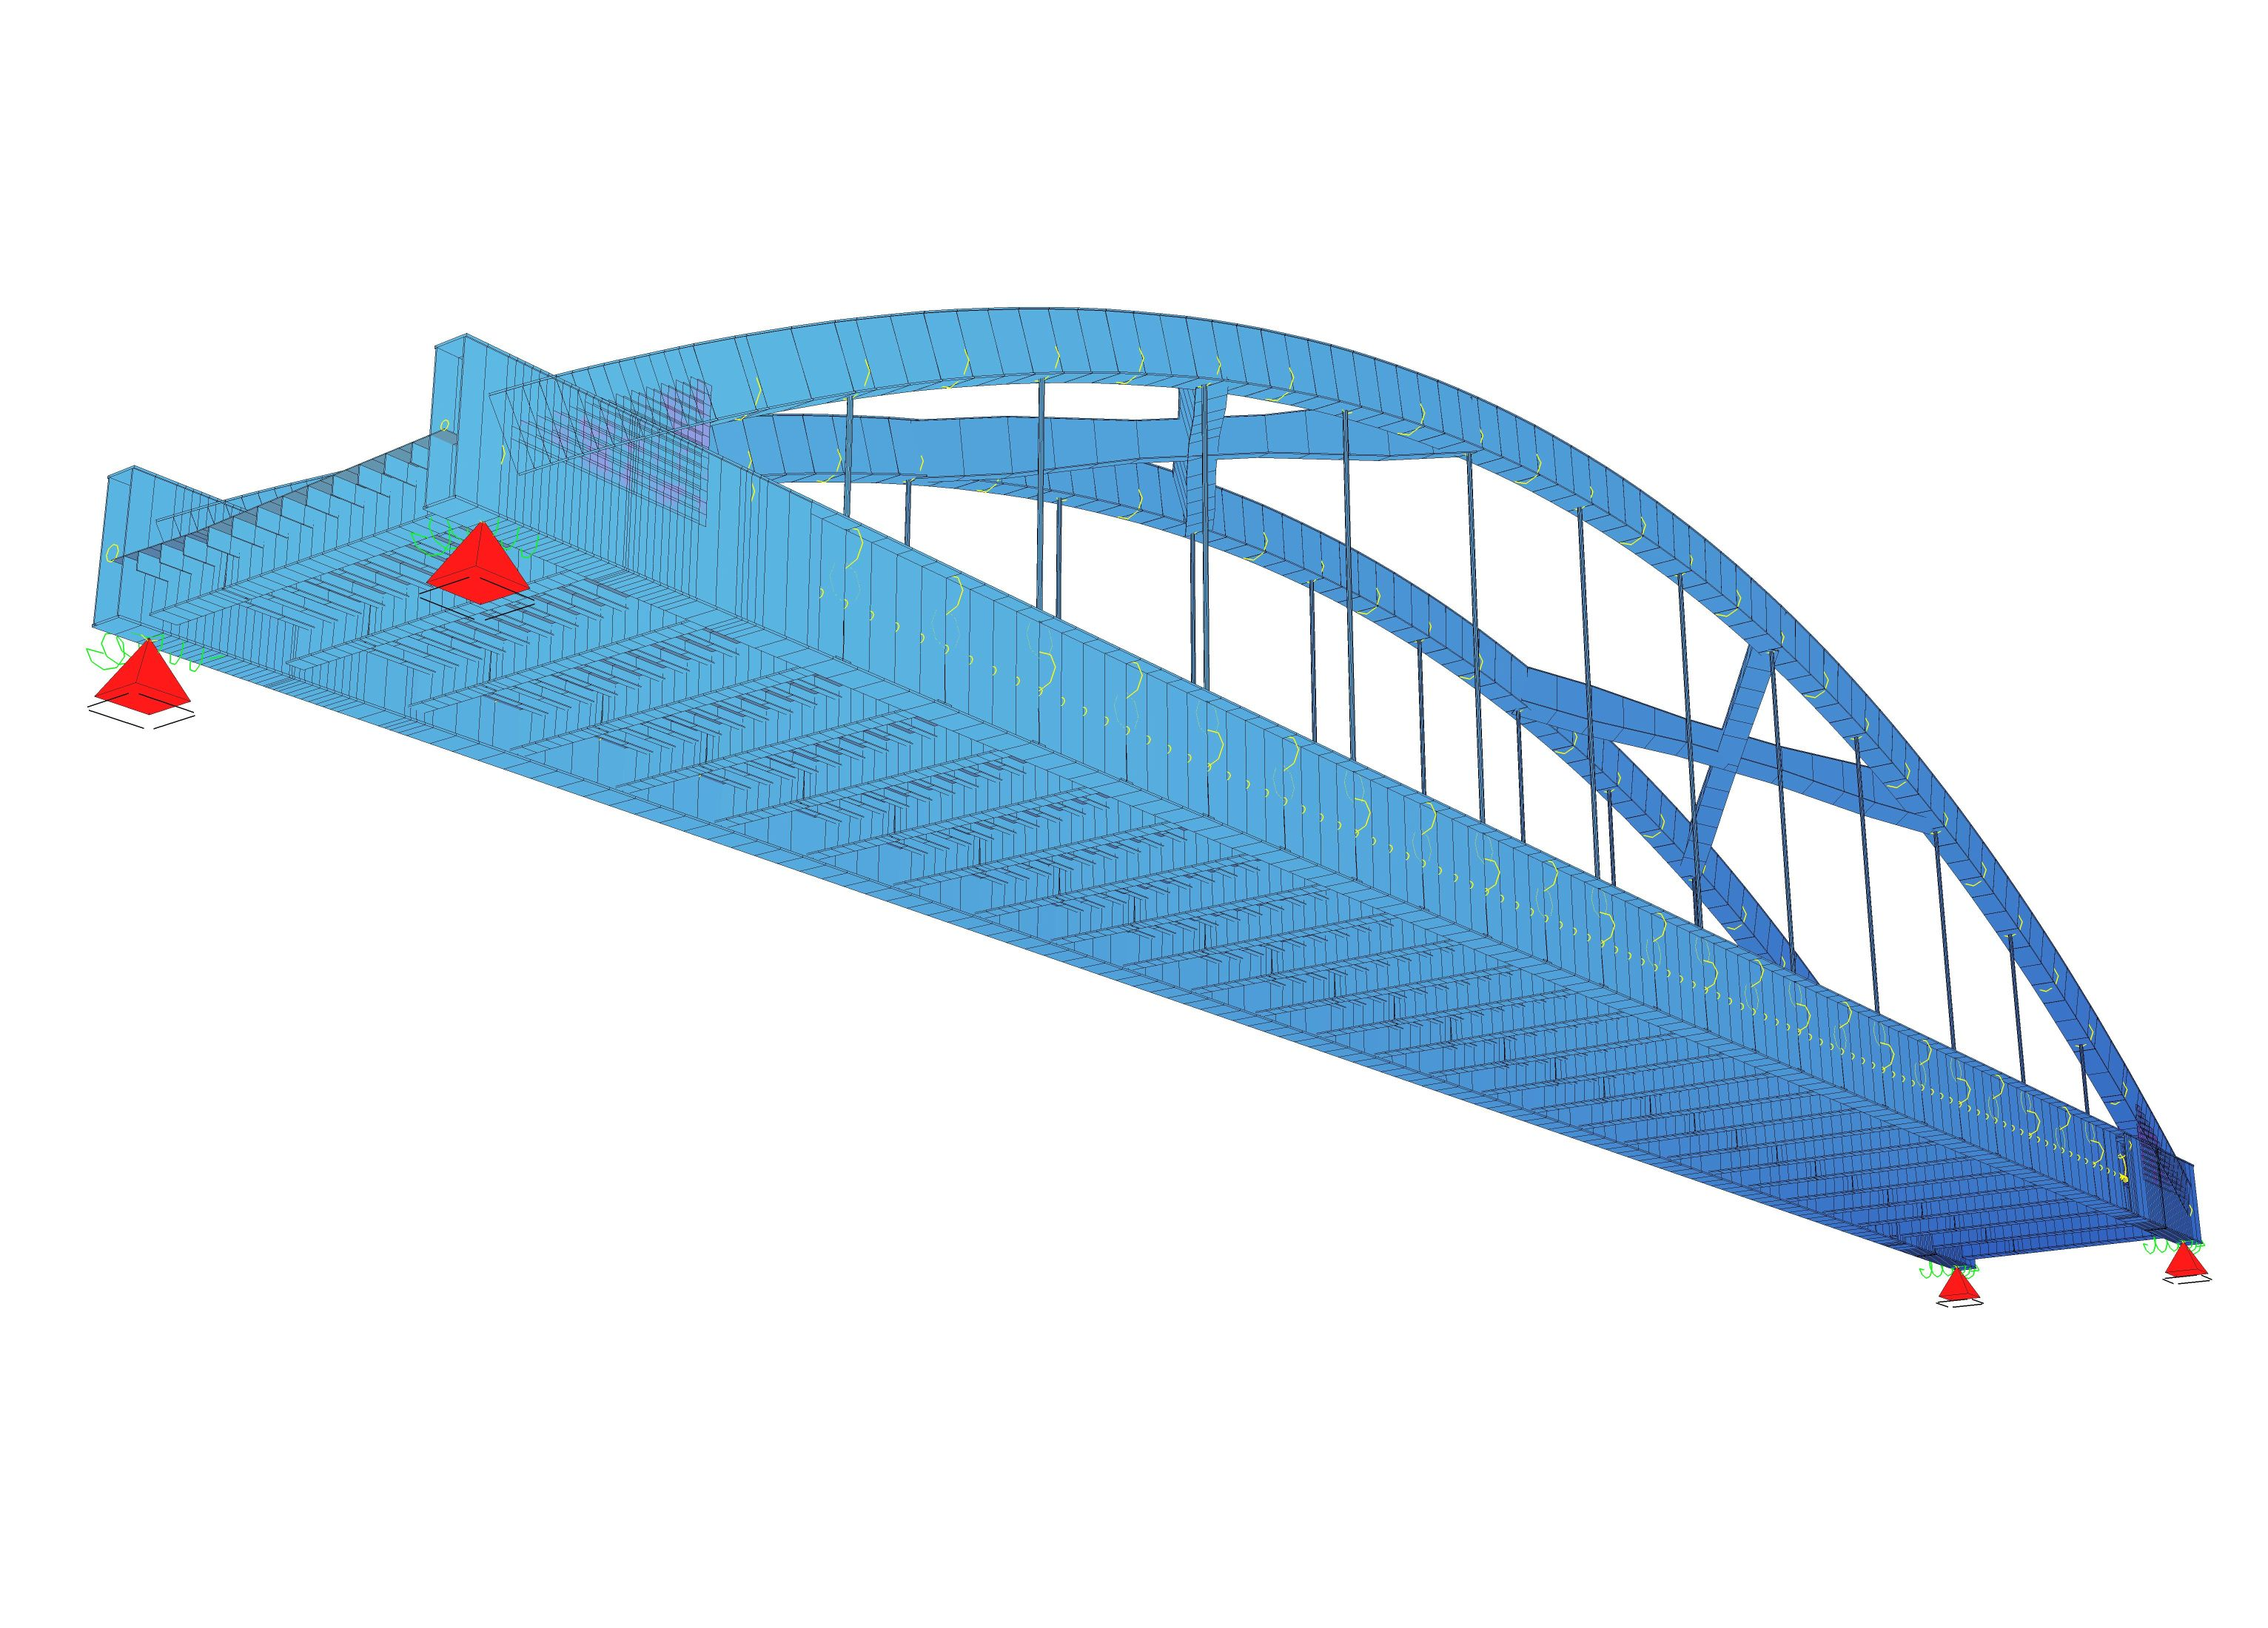
\includegraphics[width=0.5\linewidth]{/WK2/model/SCIAG_PAR_v01_vis_2.jpg}}
	\captionsetup{justification=centering}
	\caption{Wizualizacja przestrzennego modelu numerycznego wiaduktu WK2 Pomorskiej Kolei Metropolitalnej}
	\label{fig: model_wk2_visualization}
	
\end{figure}
\begin{figure}[hbt!]
	\centering
	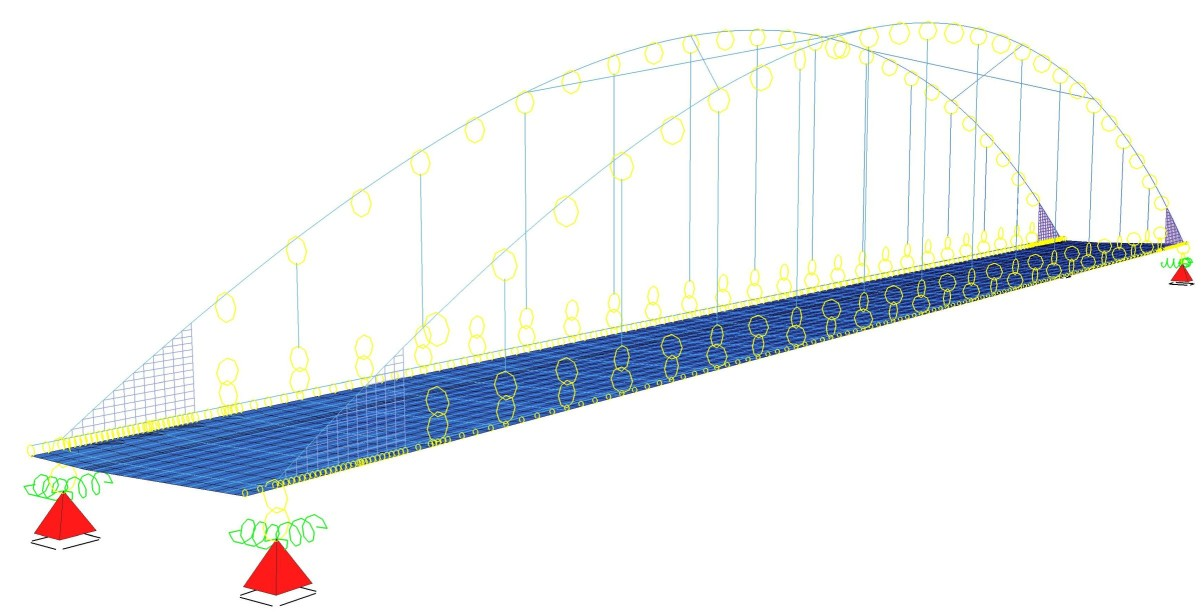
\includegraphics[width=0.8\linewidth]{/WK2/model/SCIAG_PAR_v01_schemat_1.jpg}
	\captionsetup{justification=centering}
	\caption{Schemat statyczny modelu numerycznego wiaduktu WK2 Pomorskiej Kolei Metropolitalnej}
	\label{fig: model_wk2_static_scheme}
\end{figure}

Obciążenie ciężarem własnym konstrukcji zostało wygenerowane na podstawie gęstości materiałów i geometrii elementów skończonych. Dodatkowe elementy takie jak przepony i zakotwienia wieszaków dodane zostały jako obciążenia węzłowe. Osobny przypadek obciążenia stanowi pomost roboczy dodany jako ekwiwalentne obciążenie węzłowe i momenty zginające. Wszystkie te dodatkowe obciążenia zestawiono na rysunku \ref{fig: model_wk2_add_loads}. Ostatnim obciążeniem stałym jest ciężar tłucznia. Z uwagi na ułożenie toru po łuku w planie, rozkład tłucznia na obiekcie nie jest regularną, symetryczną bryłą. Dostępna dokumentacja obiektu nie dostarcza dokładnych informacji o ułożeniu podsypki na pomoście. Podsypka została w prosty sposób zinwentaryzowana przez pomiar grubości w niektórych punktach charakterystycznych. Na rysunku \ref{fig: wk2_cross_sect} zaprezentowano zinwentaryzowany układ tłucznia w przekroju przęsłowym. Zastosowana metoda pomiaru objętości tłucznia nie jest dokładna i na pewno nie odzwierciedla realnego rozkładu ciężaru podsypki na obiekcie. Z tego względu podzielono obciążenie tłuczniem na dwa osobne przypadki: równomiernie rozłożone obciążenie na całej szerokości pomostu i obciążenie równomierne o stałej szerokości usytuowane wzdłuż osi toru (Rys. \ref{fig: model_wk2_balast_loadcase}). Wartość obciążenia tłuczniem przyjęto z normy \parencite{PKNg}. 

\begin{figure}[hbt!]
	\centering
	\subfloat[]{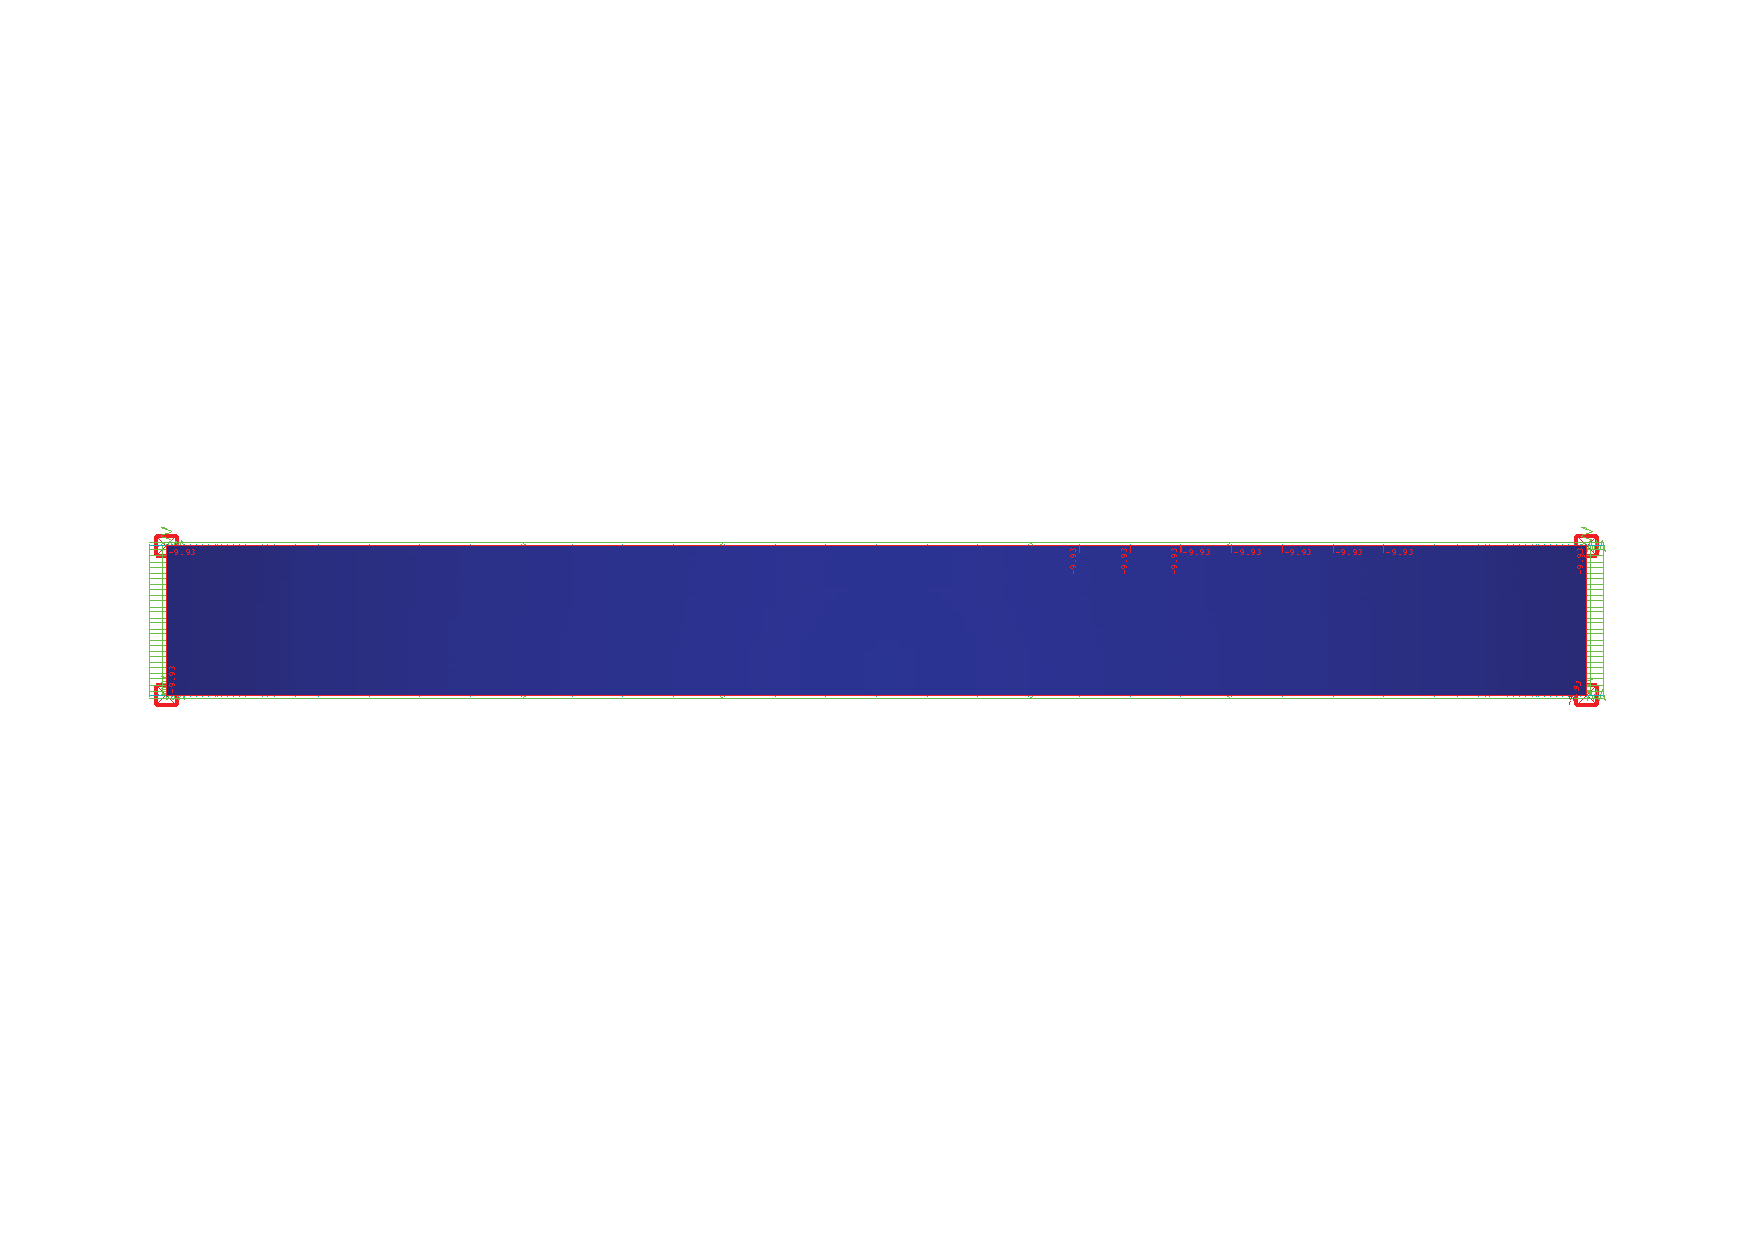
\includegraphics[width=\linewidth]{/WK2/model/tluczen_calosc.pdf}} \\
	\subfloat[]{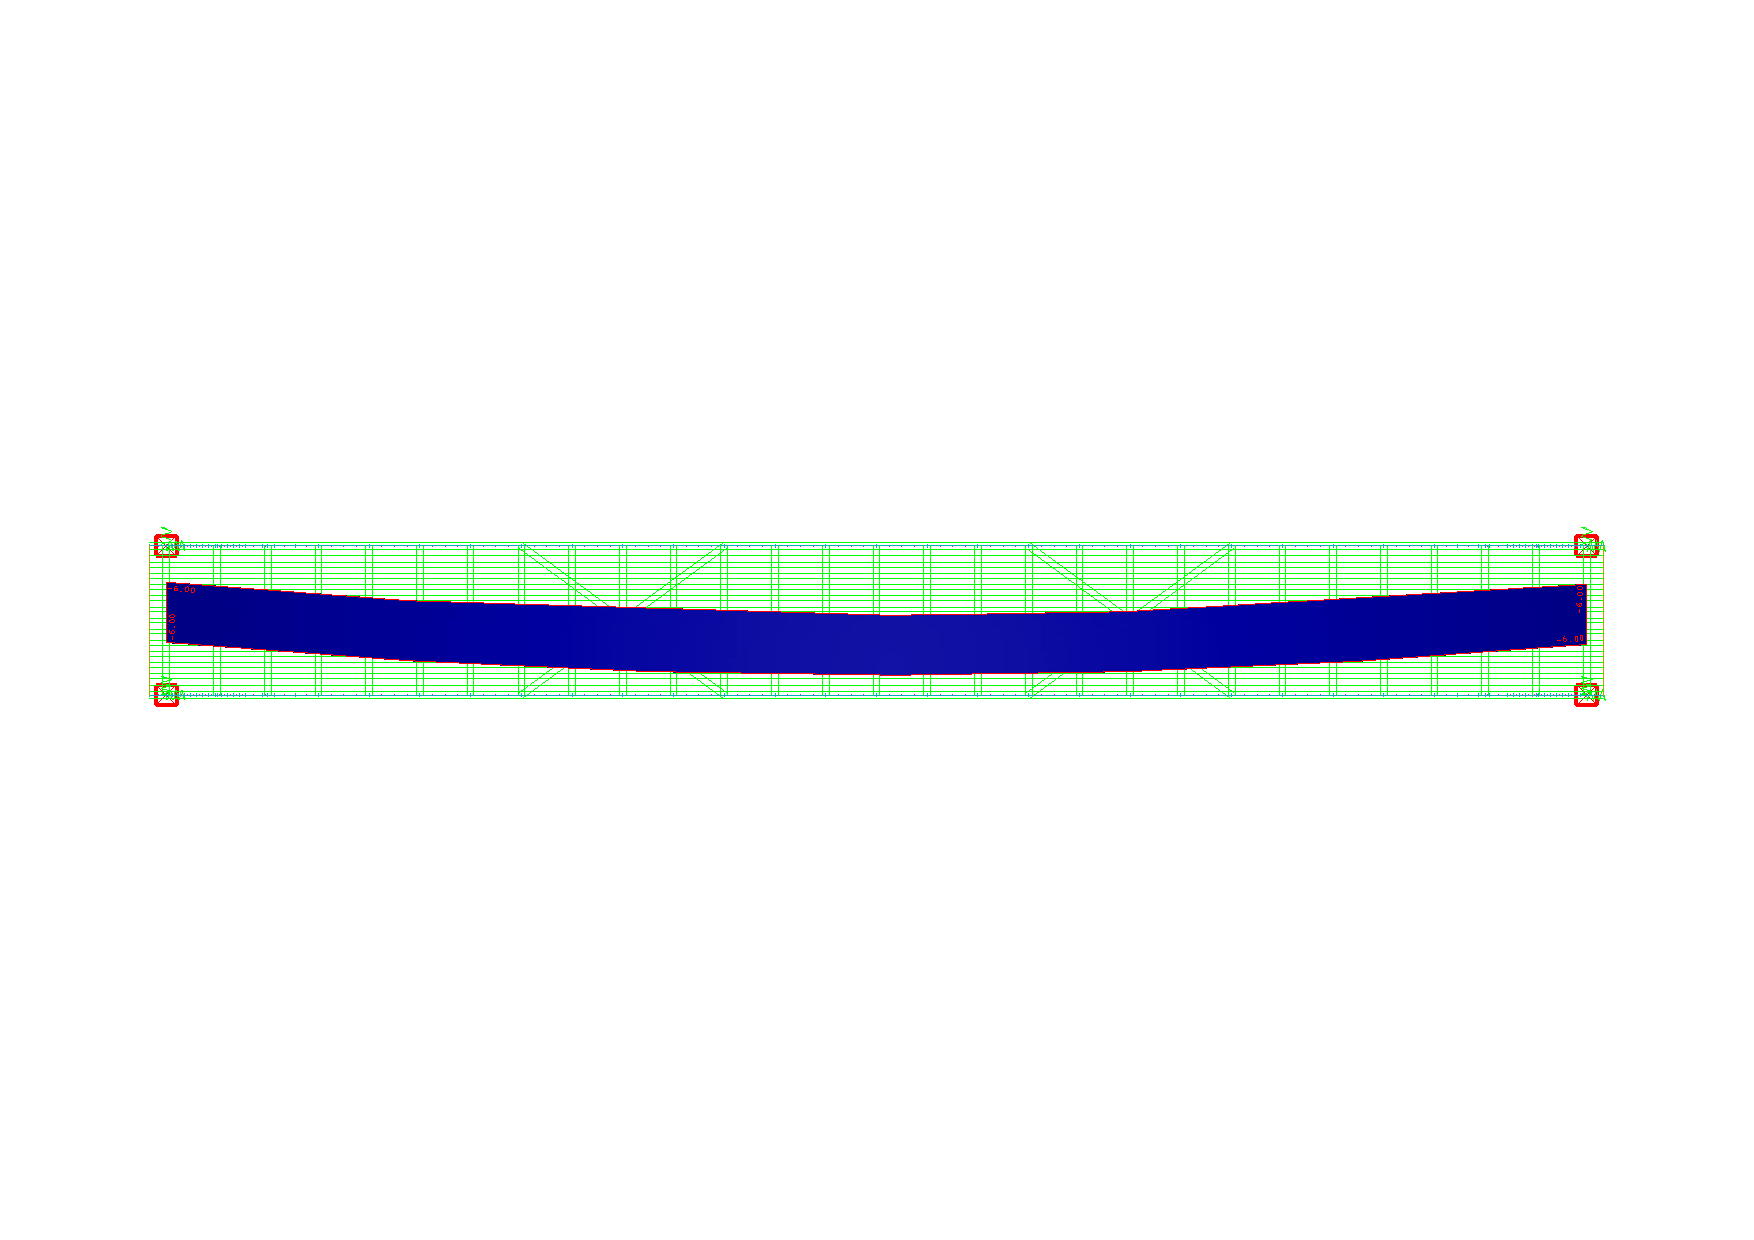
\includegraphics[width=\linewidth]{/WK2/model/tluczen_luk.pdf}}
	\captionsetup{justification=centering}
	\caption{Przyjęty kształt obciążenia tłuczniem: (a) część równomiernie rozłożona, (b) część wzdłuż osi toru}
	\label{fig: model_wk2_balast_loadcase}
\end{figure}

\begin{figure}[hbt!]
	\centering
	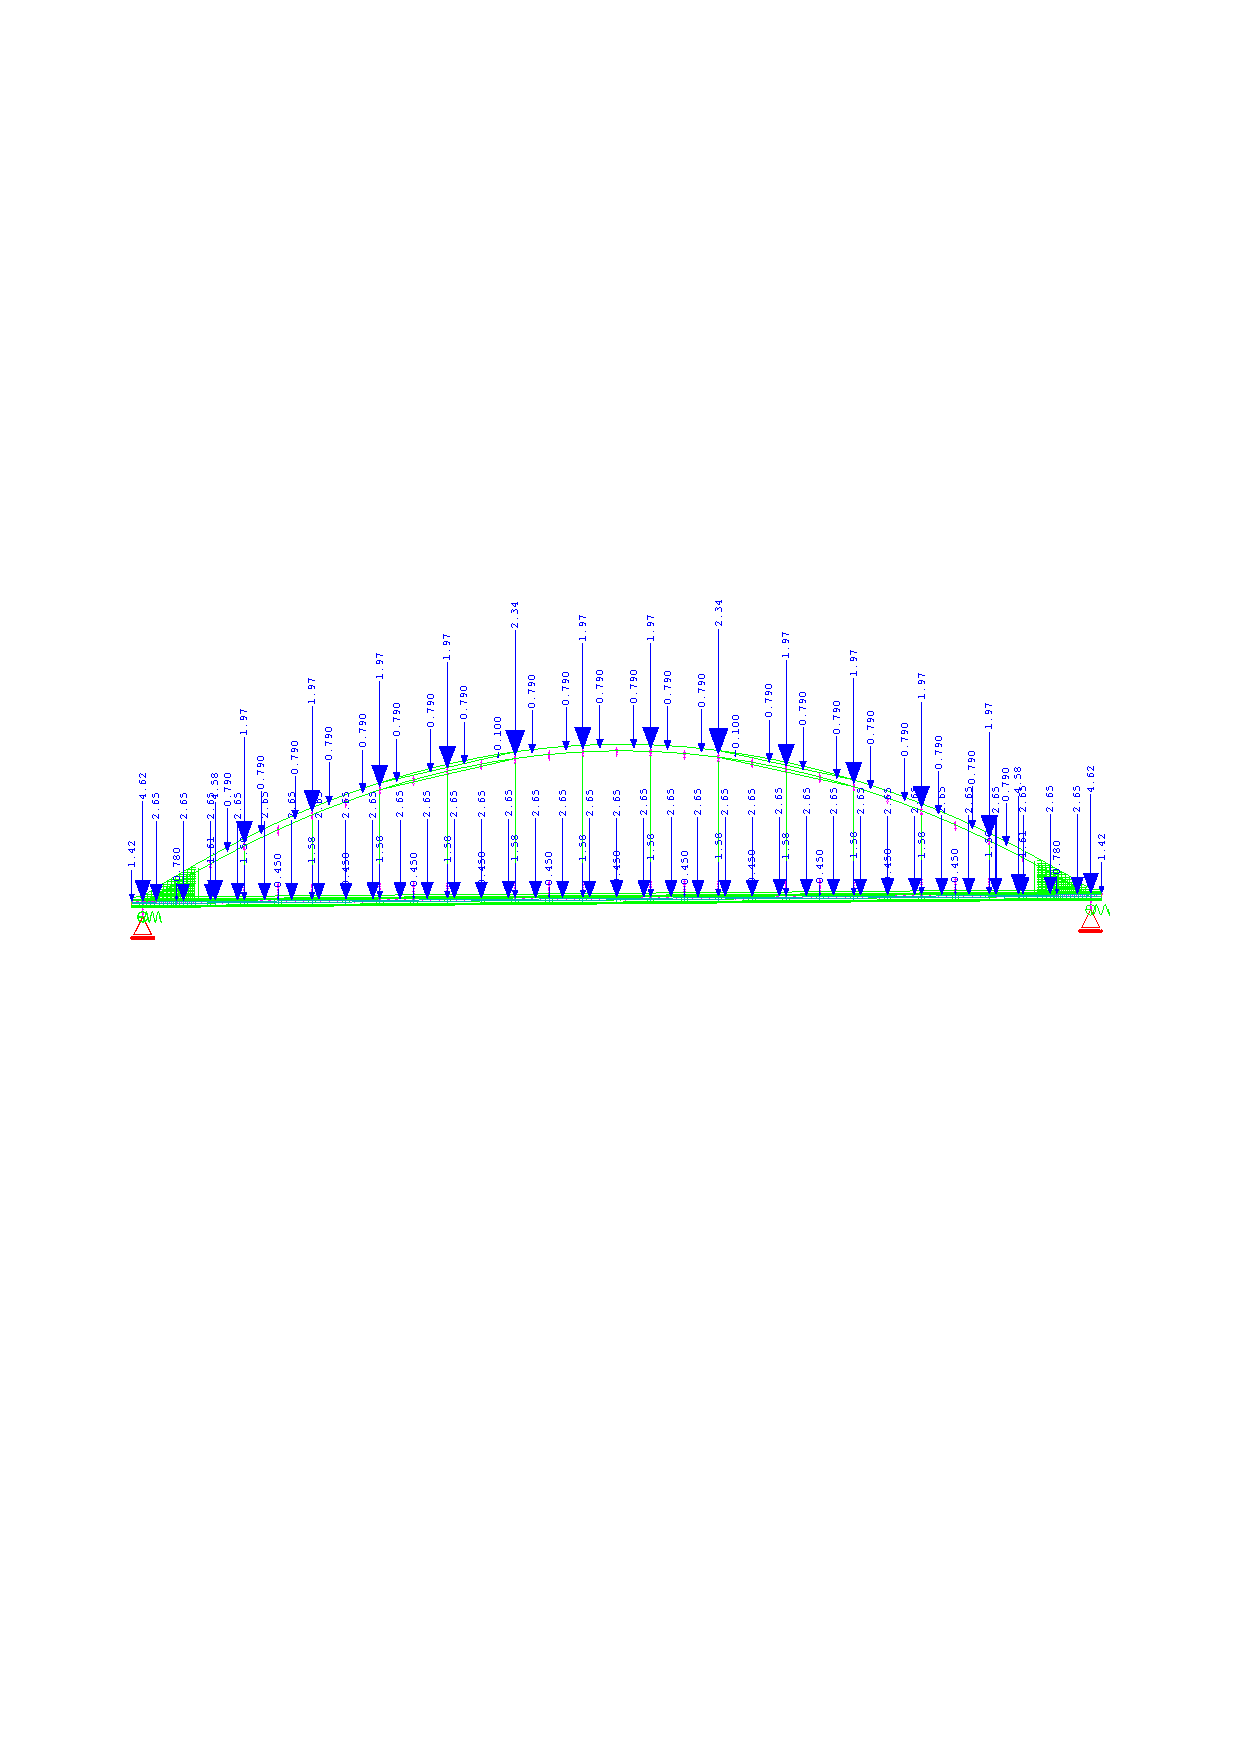
\includegraphics[width=\linewidth]{/WK2/model/model_additional_loads.pdf}
	\captionsetup{justification=centering}
	\caption{Zestawienie dodatkowych obciążeń od elementów konstrukcyjnych nie ujętych elementami skończonymi modelu}
	\label{fig: model_wk2_add_loads}
\end{figure}

Na tak przygotowanym modelu przeprowadzono teoretyczną analizę modalną. Do wyznaczenia parametrów modalnych użyto algorytmu Lanczosa. Wyznaczono pierwszych dziesięć zestawów częstotliwości i postaci drgań własnych. Rezultaty przedstawiono na rysunku \ref{fig: model_wk2_origin_mods}.




\begin{figure}[p]
	\centering
	\begin{tabular}[c]{c}
		\subfloat[Mod 1, $f_1=1.408\text{ Hz}$]{\label{fig: wk2_origin_mod01}%
			\begin{tabular}[b]{c c}
				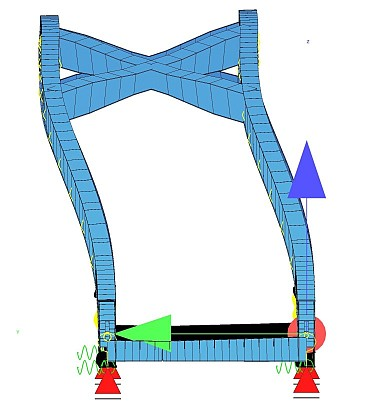
\includegraphics[height=0.12\textheight]{/WK2/model/mod_origin/f1f.jpg}%
				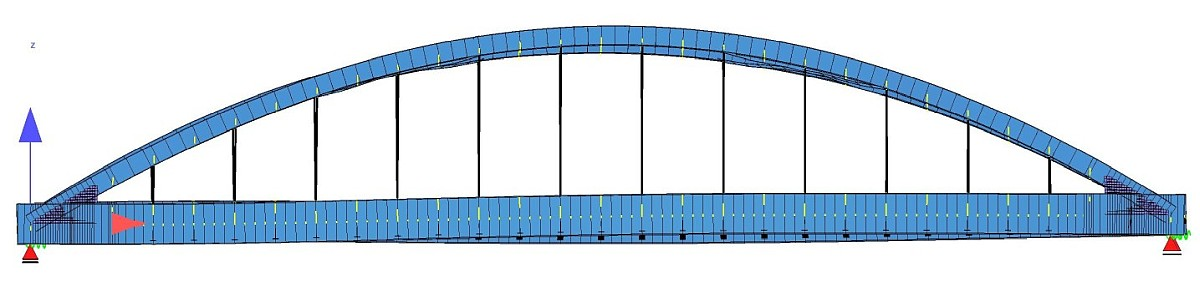
\includegraphics[width=0.7\textwidth]{/WK2/model/mod_origin/f1s.jpg}%
		\end{tabular}}\\
		\subfloat[Mod 2, $f_2=2.469 \text{ Hz}$]{\label{fig: wk2_origin_mod02}%
		\begin{tabular}[b]{c c}
			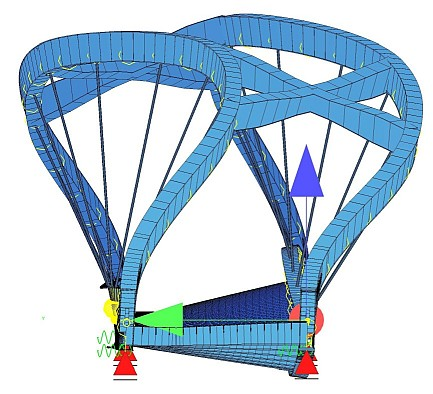
\includegraphics[height=0.12\textheight]{/WK2/model/mod_origin/f2f.jpg}%
			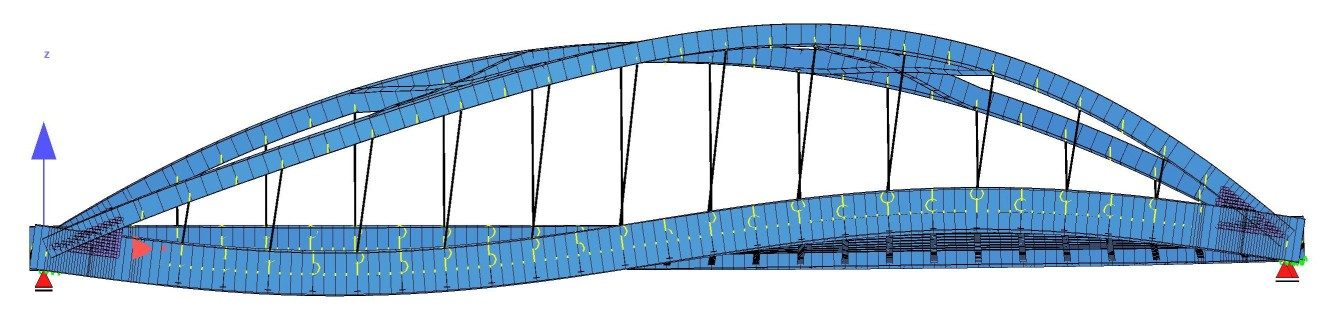
\includegraphics[width=0.7\textwidth]{/WK2/model/mod_origin/f2s.jpg}%
		\end{tabular}}\\
			\subfloat[Mod 3, $f_3=2.509 \text{ Hz}$]{\label{fig: wk2_origin_mod03}%
		\begin{tabular}[b]{c c}
			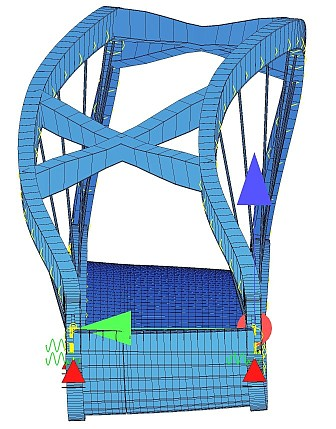
\includegraphics[height=0.12\textheight]{/WK2/model/mod_origin/f3f.jpg}%
			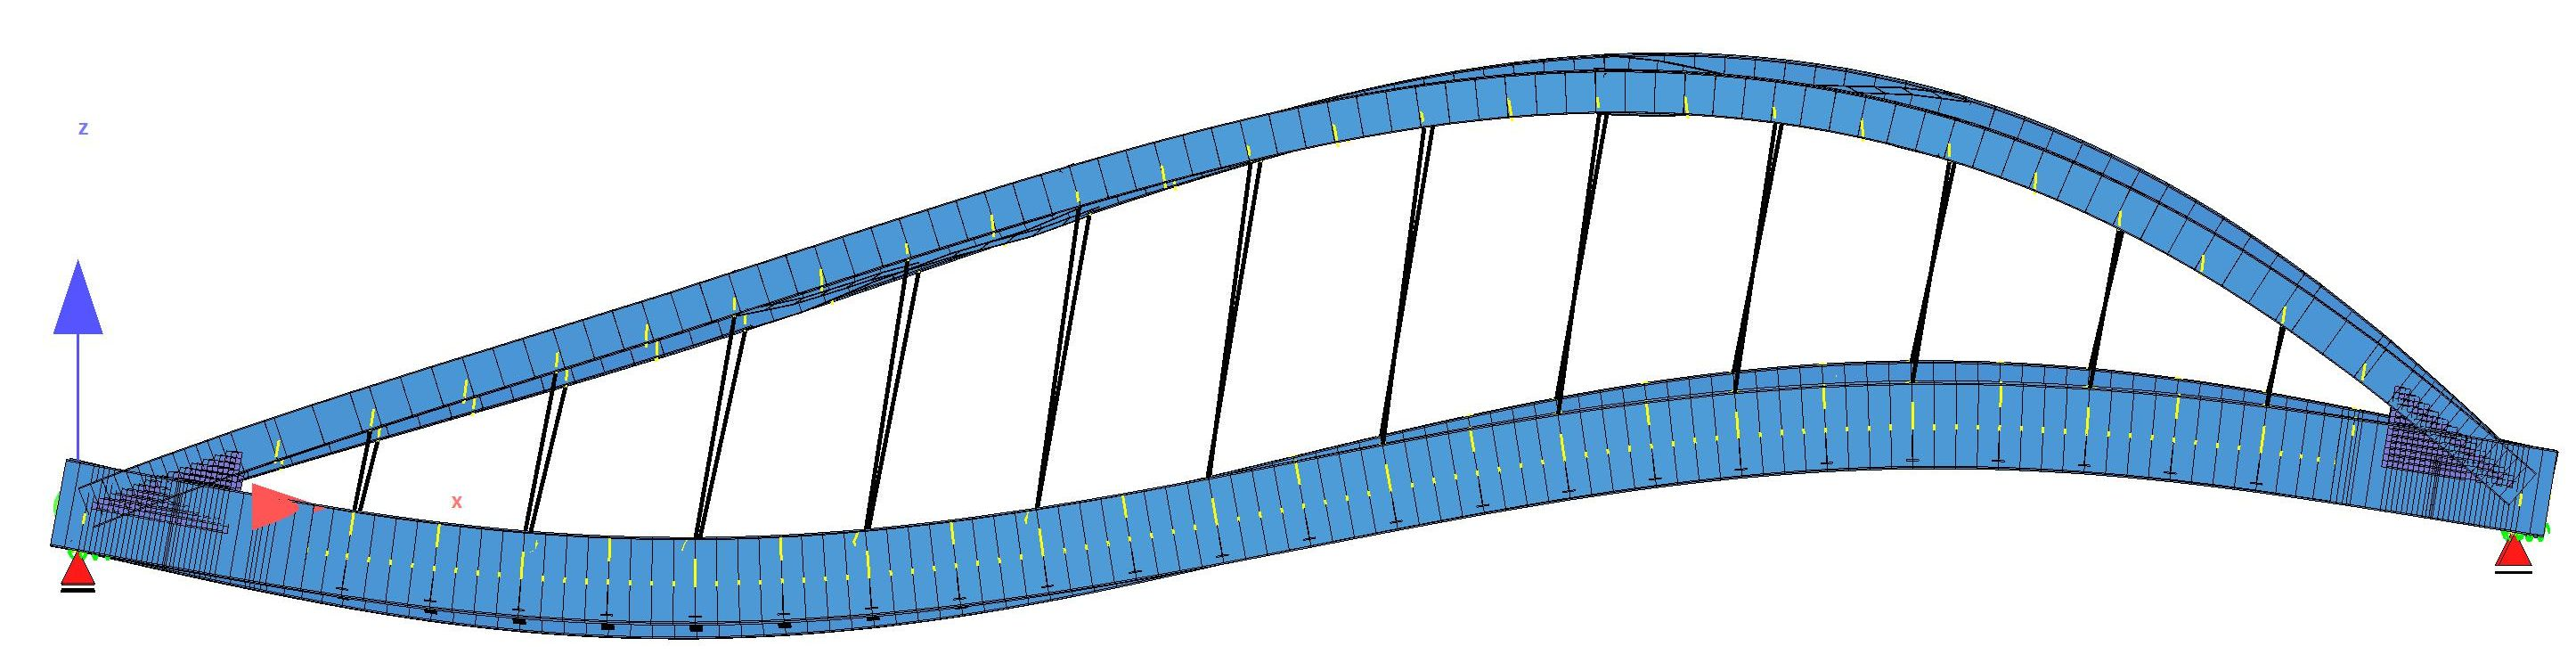
\includegraphics[width=0.7\textwidth]{/WK2/model/mod_origin/f3s.jpg}%
	\end{tabular}}\\
		\subfloat[Mod 4, $f_4=3.166 \text{ Hz}$]{\label{fig: wk2_origin_mod04}%
	\begin{tabular}[b]{c c}
		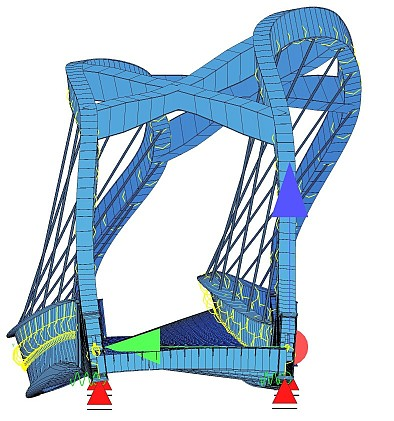
\includegraphics[height=0.12\textheight]{/WK2/model/mod_origin/f4f.jpg}%
		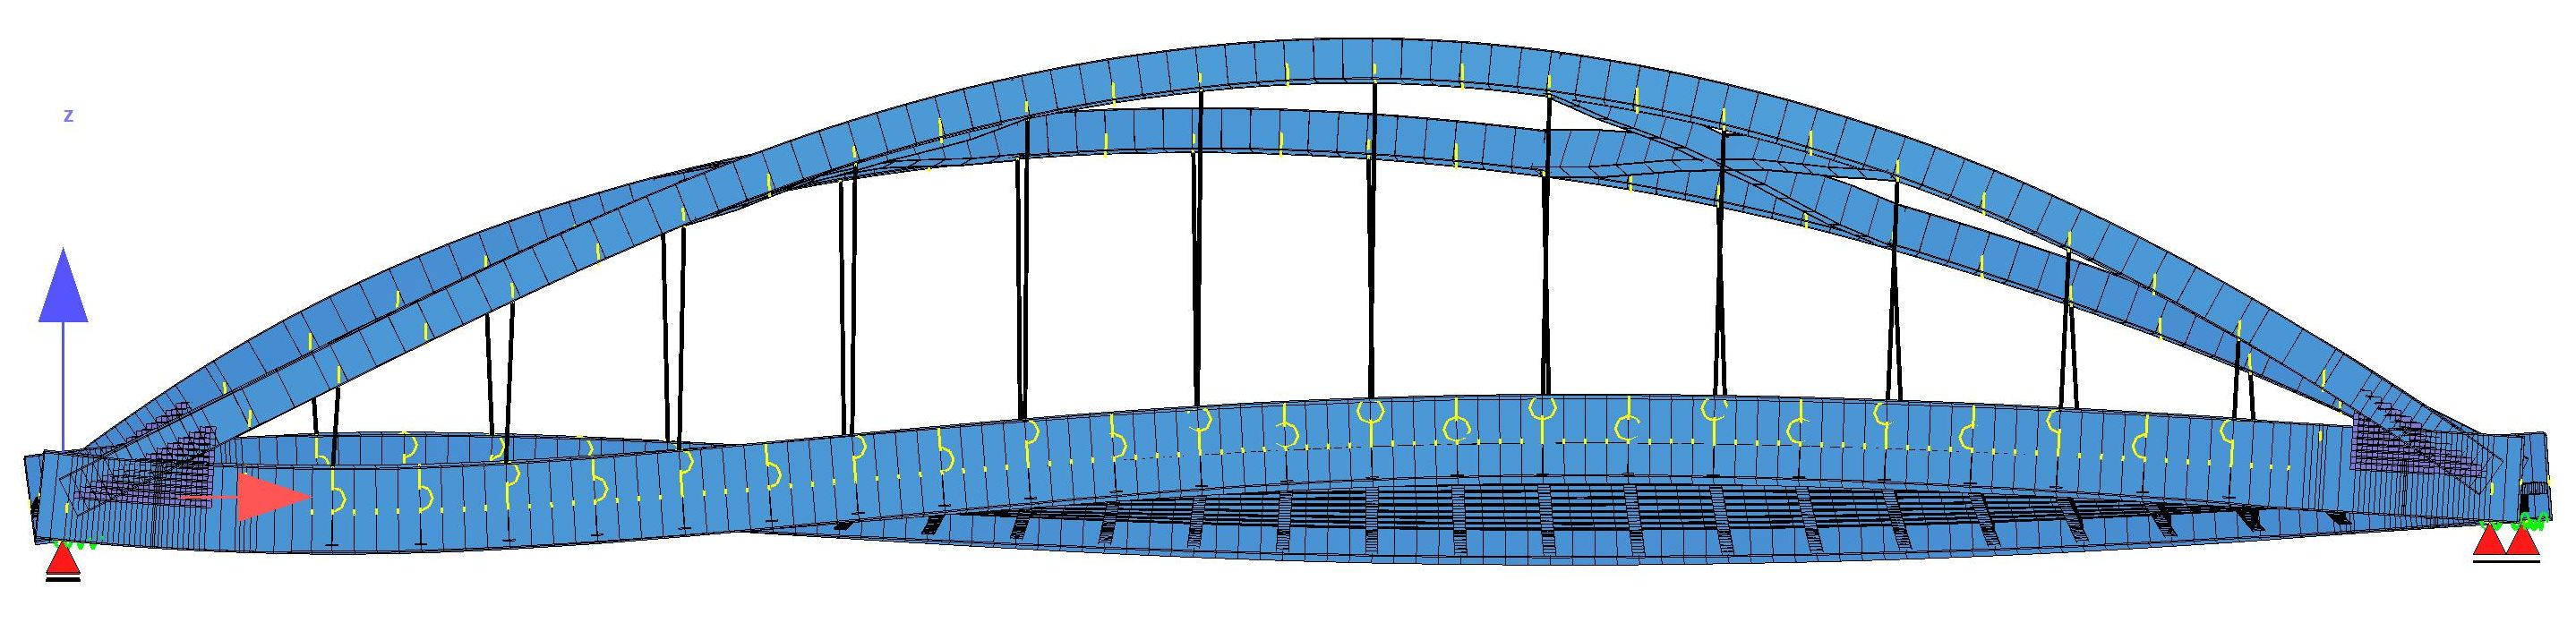
\includegraphics[width=0.7\textwidth]{/WK2/model/mod_origin/f4s.jpg}%
\end{tabular}}\\
		\subfloat[Mod 5, $f_5=3.515 \text{ Hz}$]{\label{fig: wk2_origin_mod05}%
	\begin{tabular}[b]{c c}
		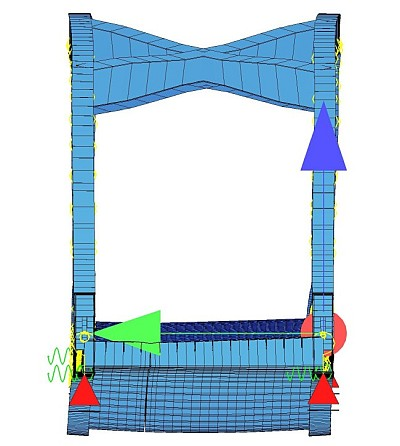
\includegraphics[height=0.12\textheight]{/WK2/model/mod_origin/f5f.jpg}%
		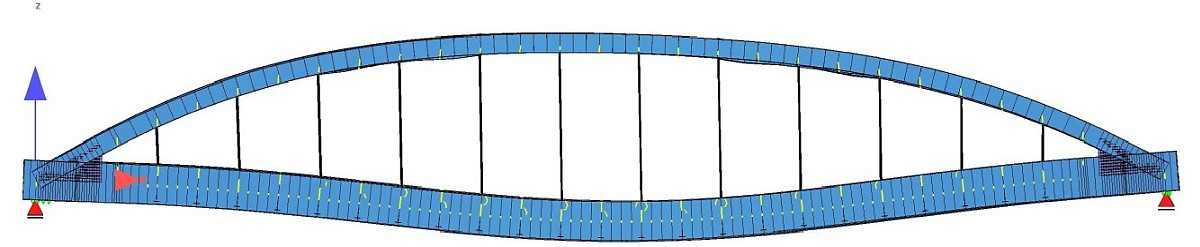
\includegraphics[width=0.7\textwidth]{/WK2/model/mod_origin/f5s.jpg}%
\end{tabular}}\\
		\subfloat[Mod 6, $f_6=5.031 \text{ Hz}$]{\label{fig: wk2_origin_mod06}%
	\begin{tabular}[b]{c c}
		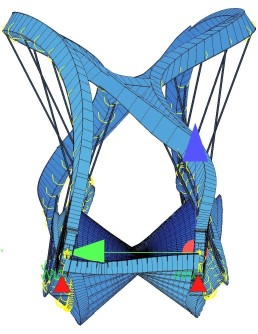
\includegraphics[height=0.12\textheight]{/WK2/model/mod_origin/f6f.jpg}%
		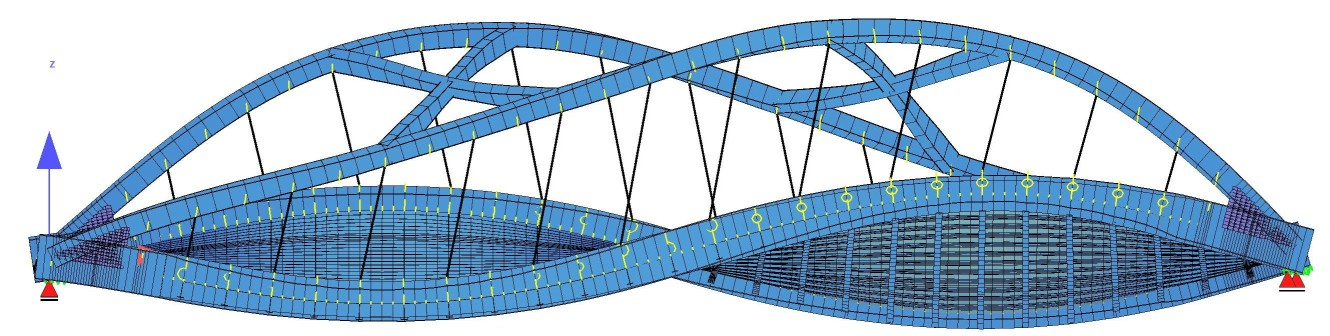
\includegraphics[width=0.7\textwidth]{/WK2/model/mod_origin/f6s.jpg}%
\end{tabular}}\\
	\end{tabular}
	\caption{Postaci i częstotliwości drgań własnych wiaduktu WK2 - Model wstępny}
	\label{fig: model_wk2_origin_mods}
\end{figure}

\begin{figure}[H]\ContinuedFloat
	\centering
	\begin{tabular}[c]{c}
		\subfloat[Mod 7, $f_7=5.584 \text{ Hz}$]{\label{fig: wk2_origin_mod07}%
			\begin{tabular}[b]{c c}
				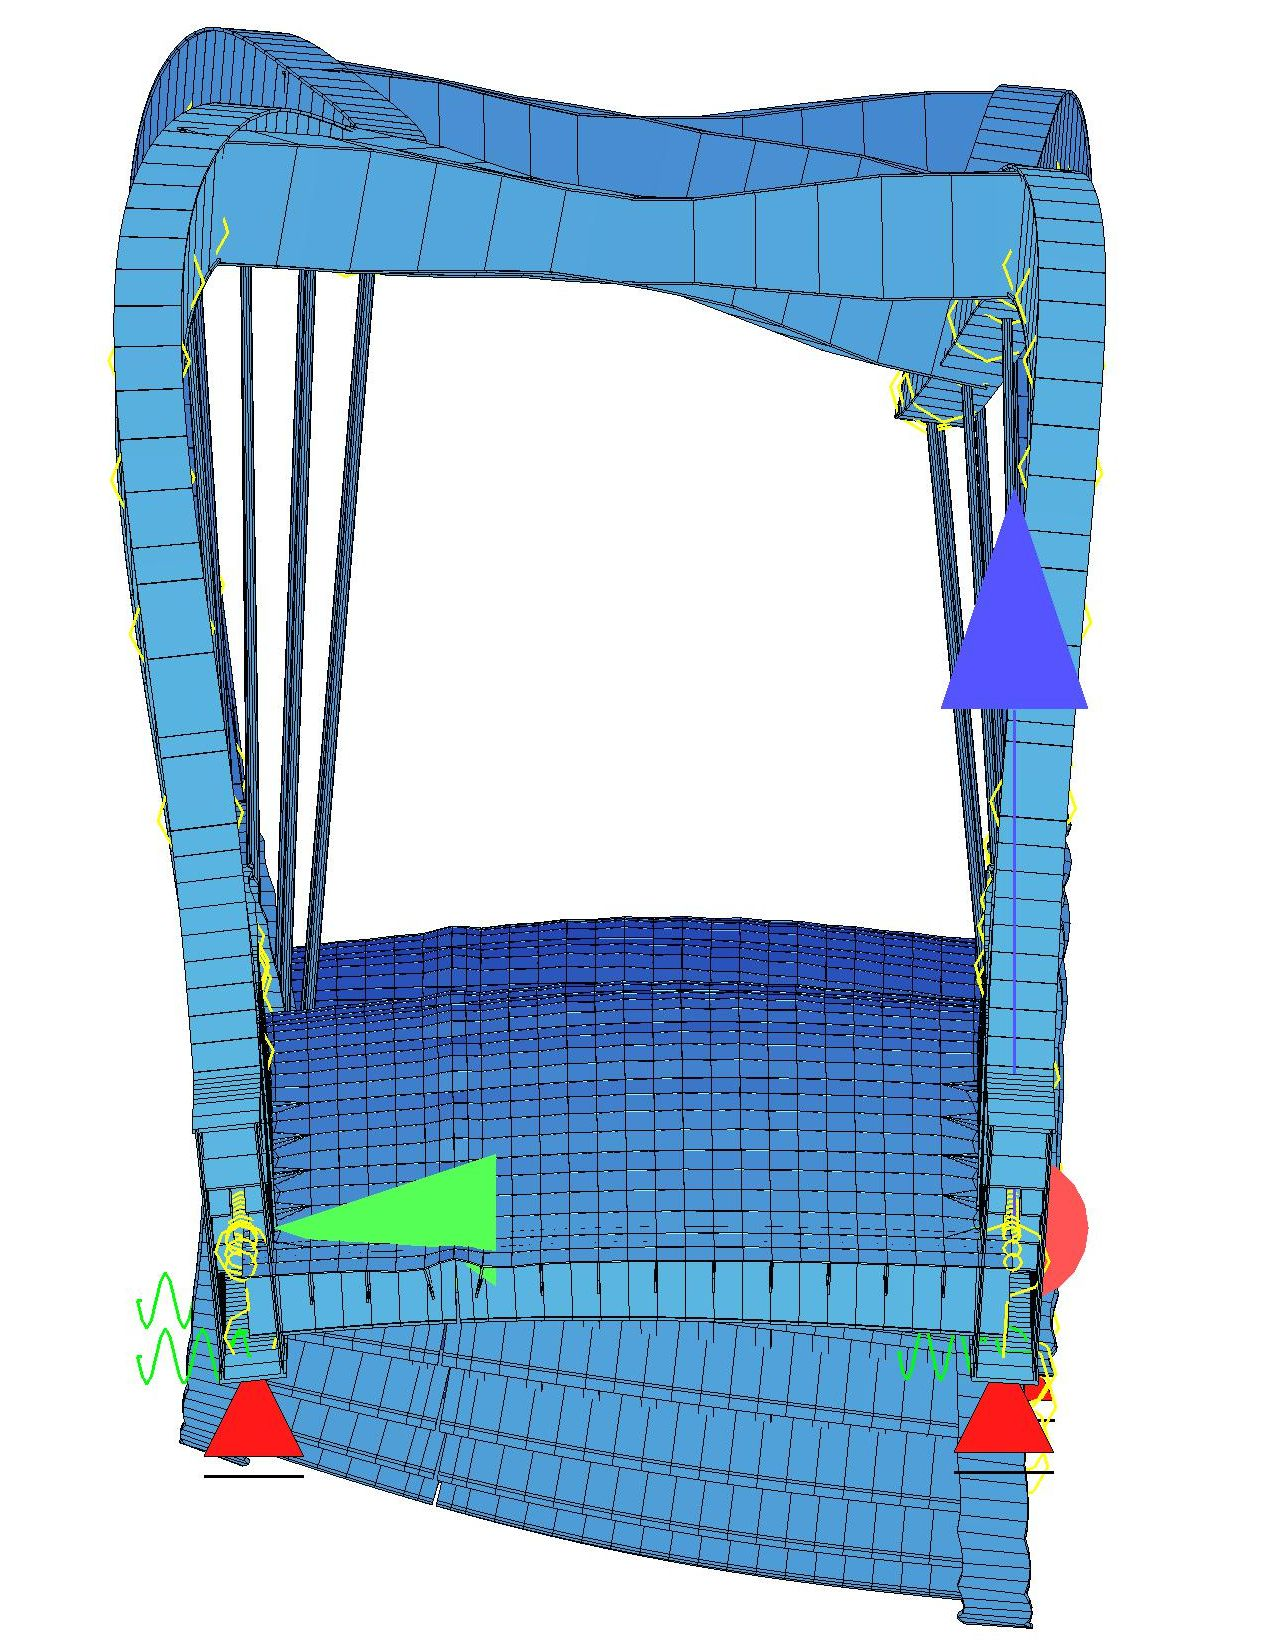
\includegraphics[height=0.12\textheight]{/WK2/model/mod_origin/f7f.jpg}%
				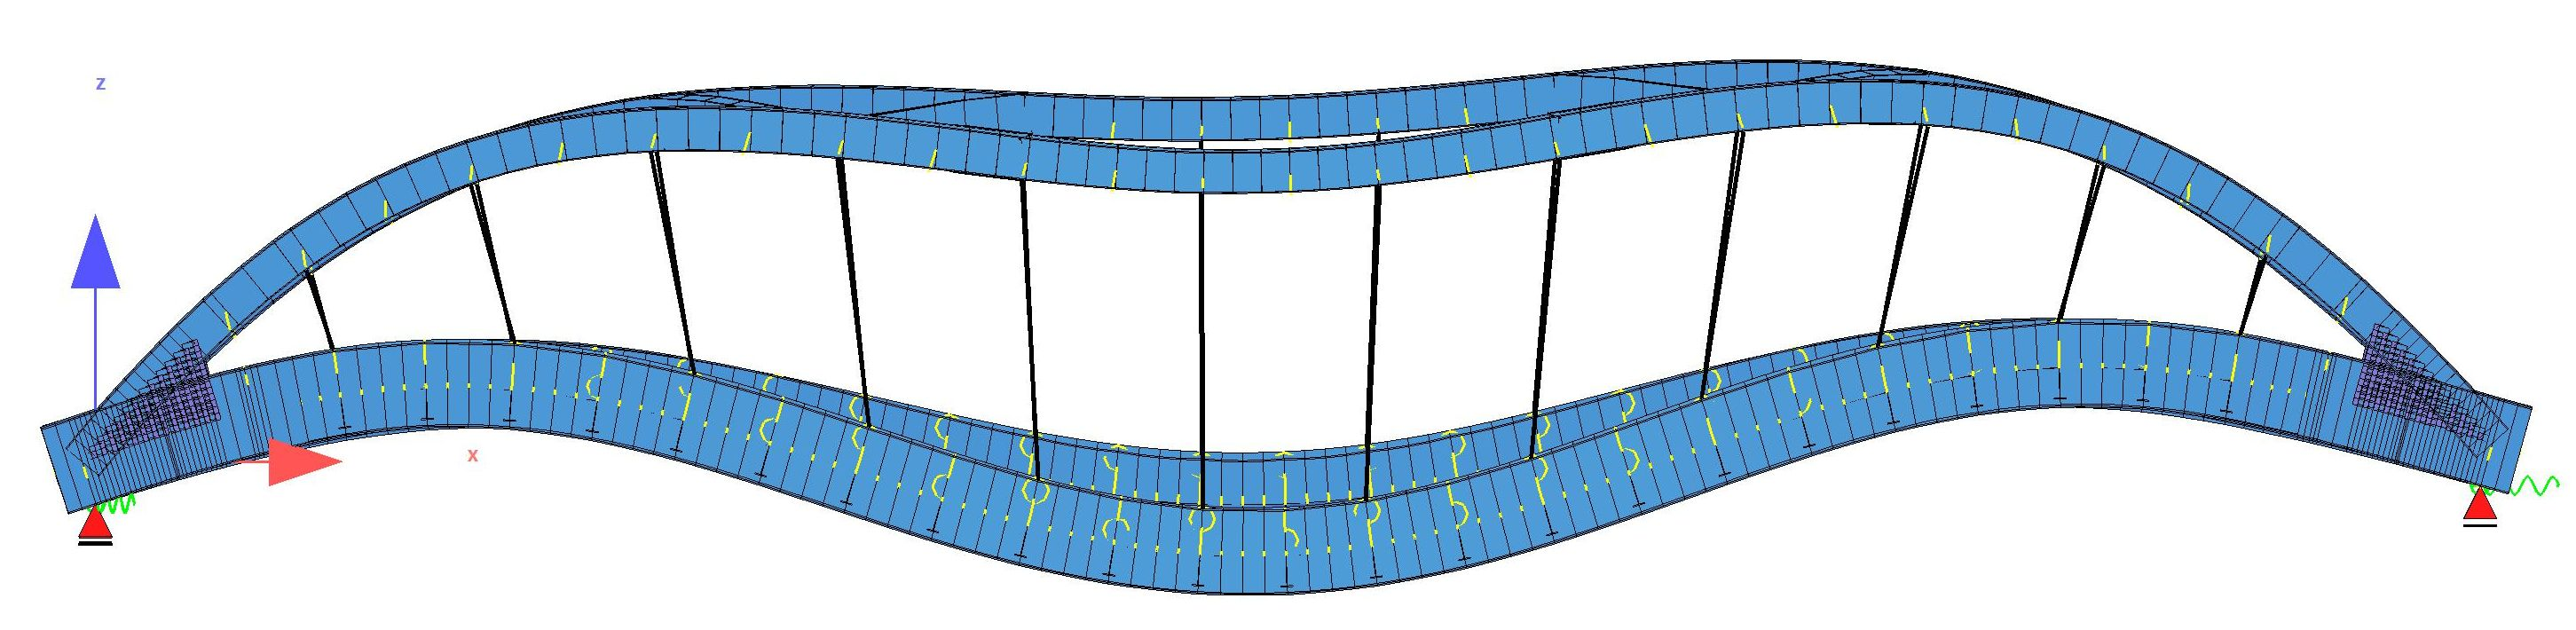
\includegraphics[width=0.7\textwidth]{/WK2/model/mod_origin/f7s.jpg}%
		\end{tabular}}\\
		\subfloat[Mod 8, $f_8=5.874 \text{ Hz}$]{\label{fig: wk2_origin_mod08}%
			\begin{tabular}[b]{c c}
				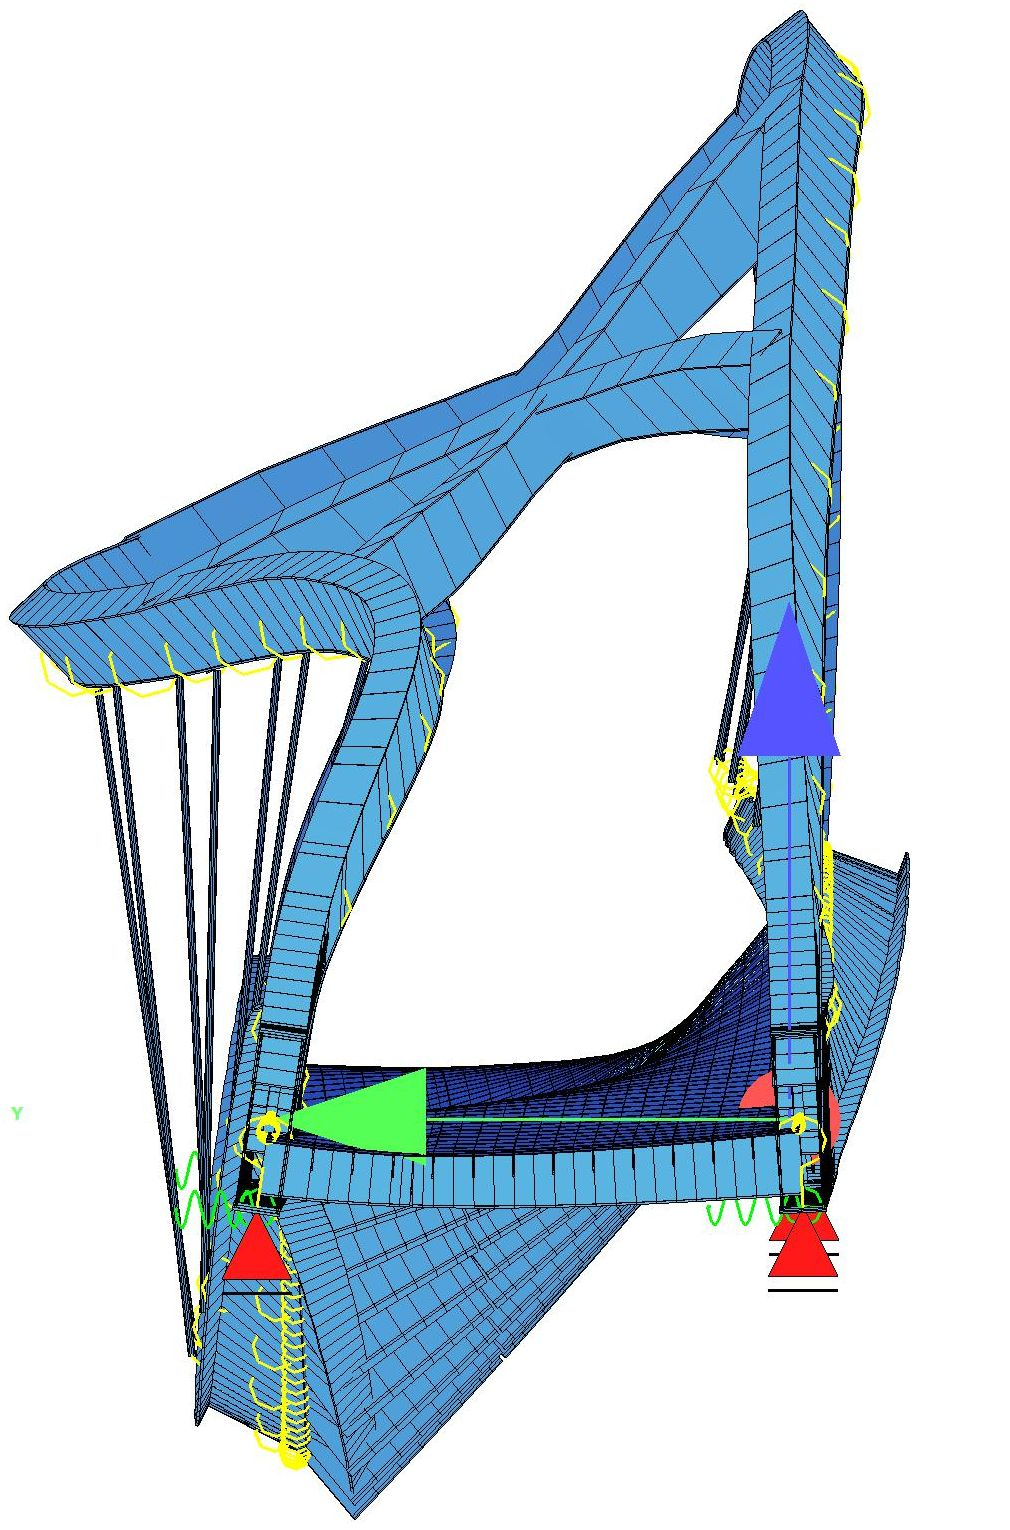
\includegraphics[height=0.12\textheight]{/WK2/model/mod_origin/f8f.jpg}%
				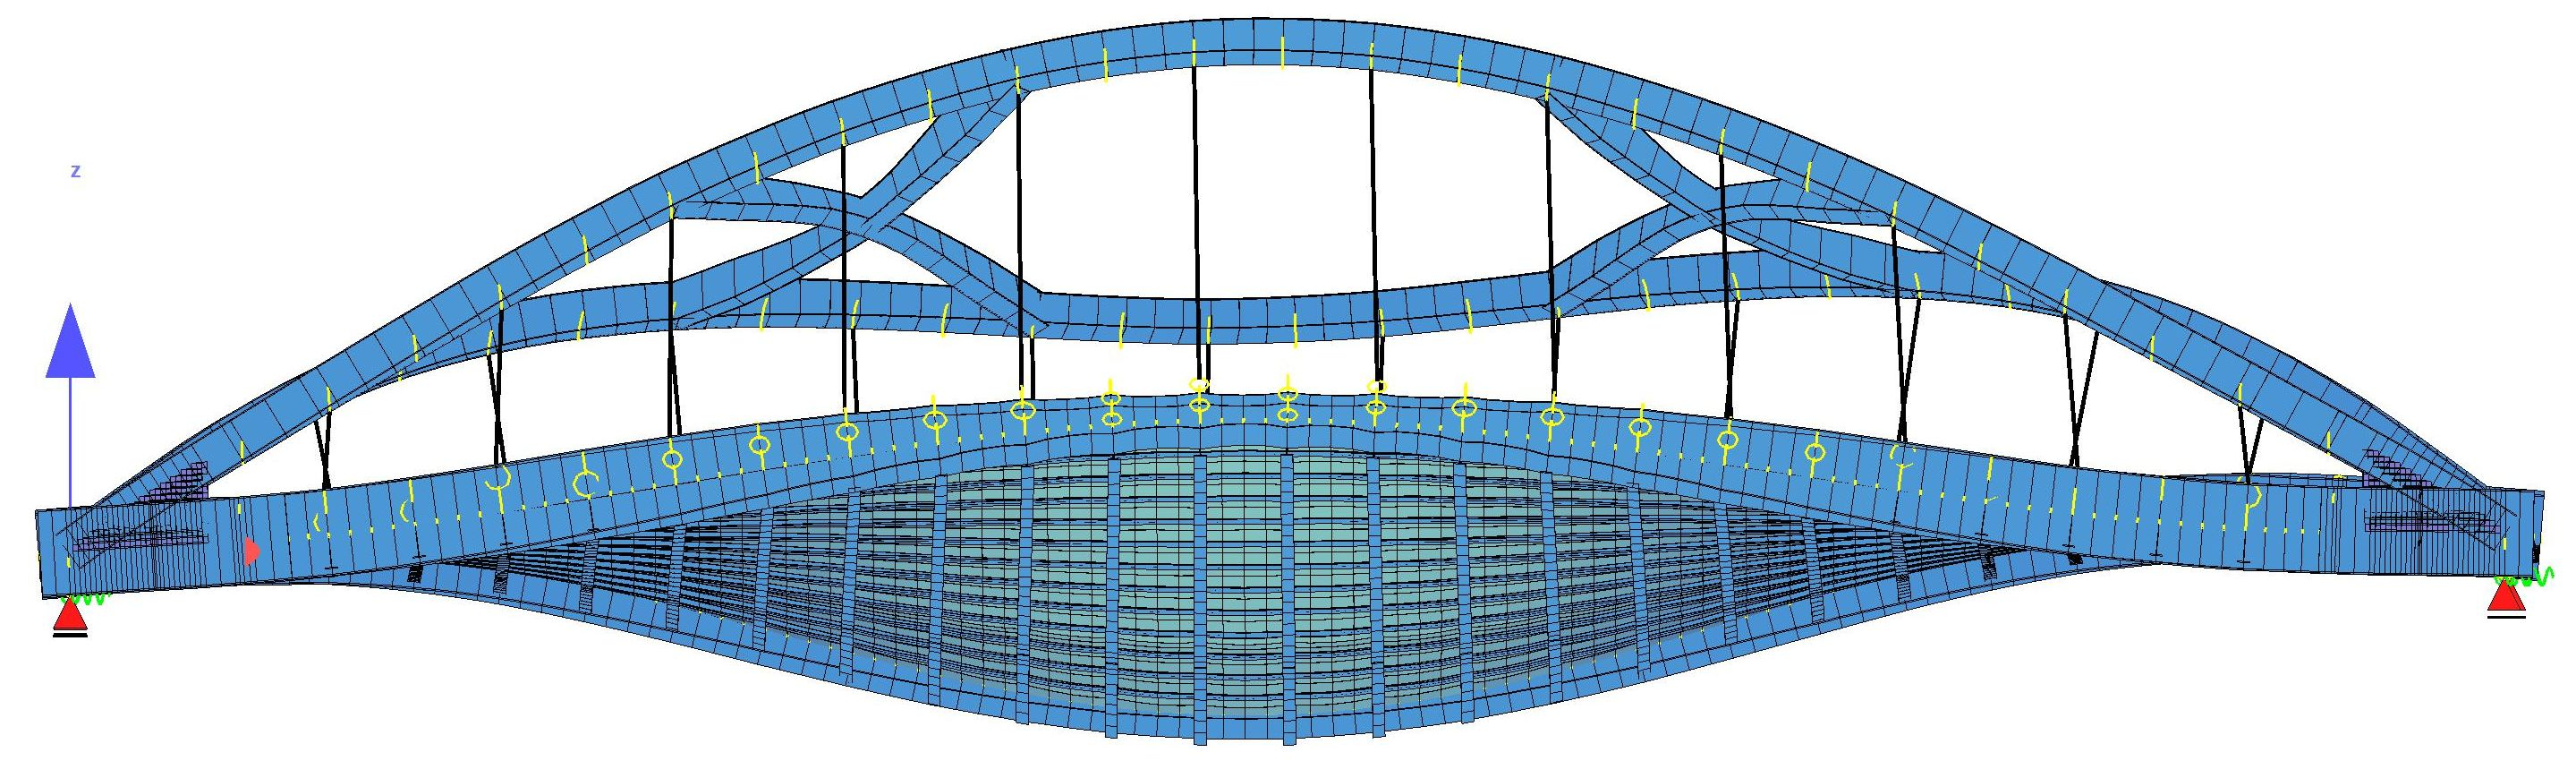
\includegraphics[width=0.7\textwidth]{/WK2/model/mod_origin/f8s.jpg}%
		\end{tabular}}\\
		\subfloat[Mod 9, $f_9=6.064 \text{ Hz}$]{\label{fig: wk2_origin_mod09}%
			\begin{tabular}[b]{c c}
				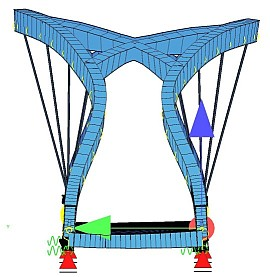
\includegraphics[height=0.12\textheight]{/WK2/model/mod_origin/f9f.jpg}%
				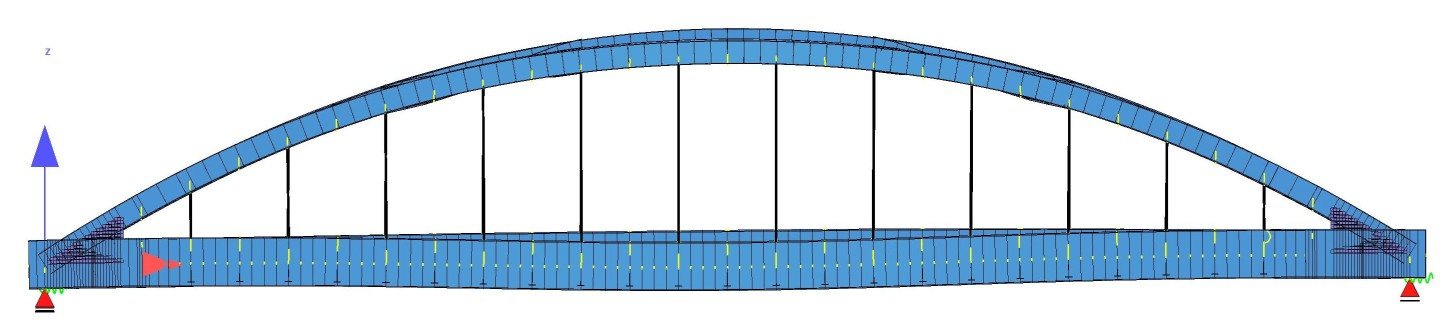
\includegraphics[width=0.7\textwidth]{/WK2/model/mod_origin/f9s.jpg}%
		\end{tabular}}\\
		\subfloat[Mod 10, $f_{10}=7.860 \text{ Hz}$]{\label{fig: wk2_origin_mod10}%
			\begin{tabular}[b]{c c}
				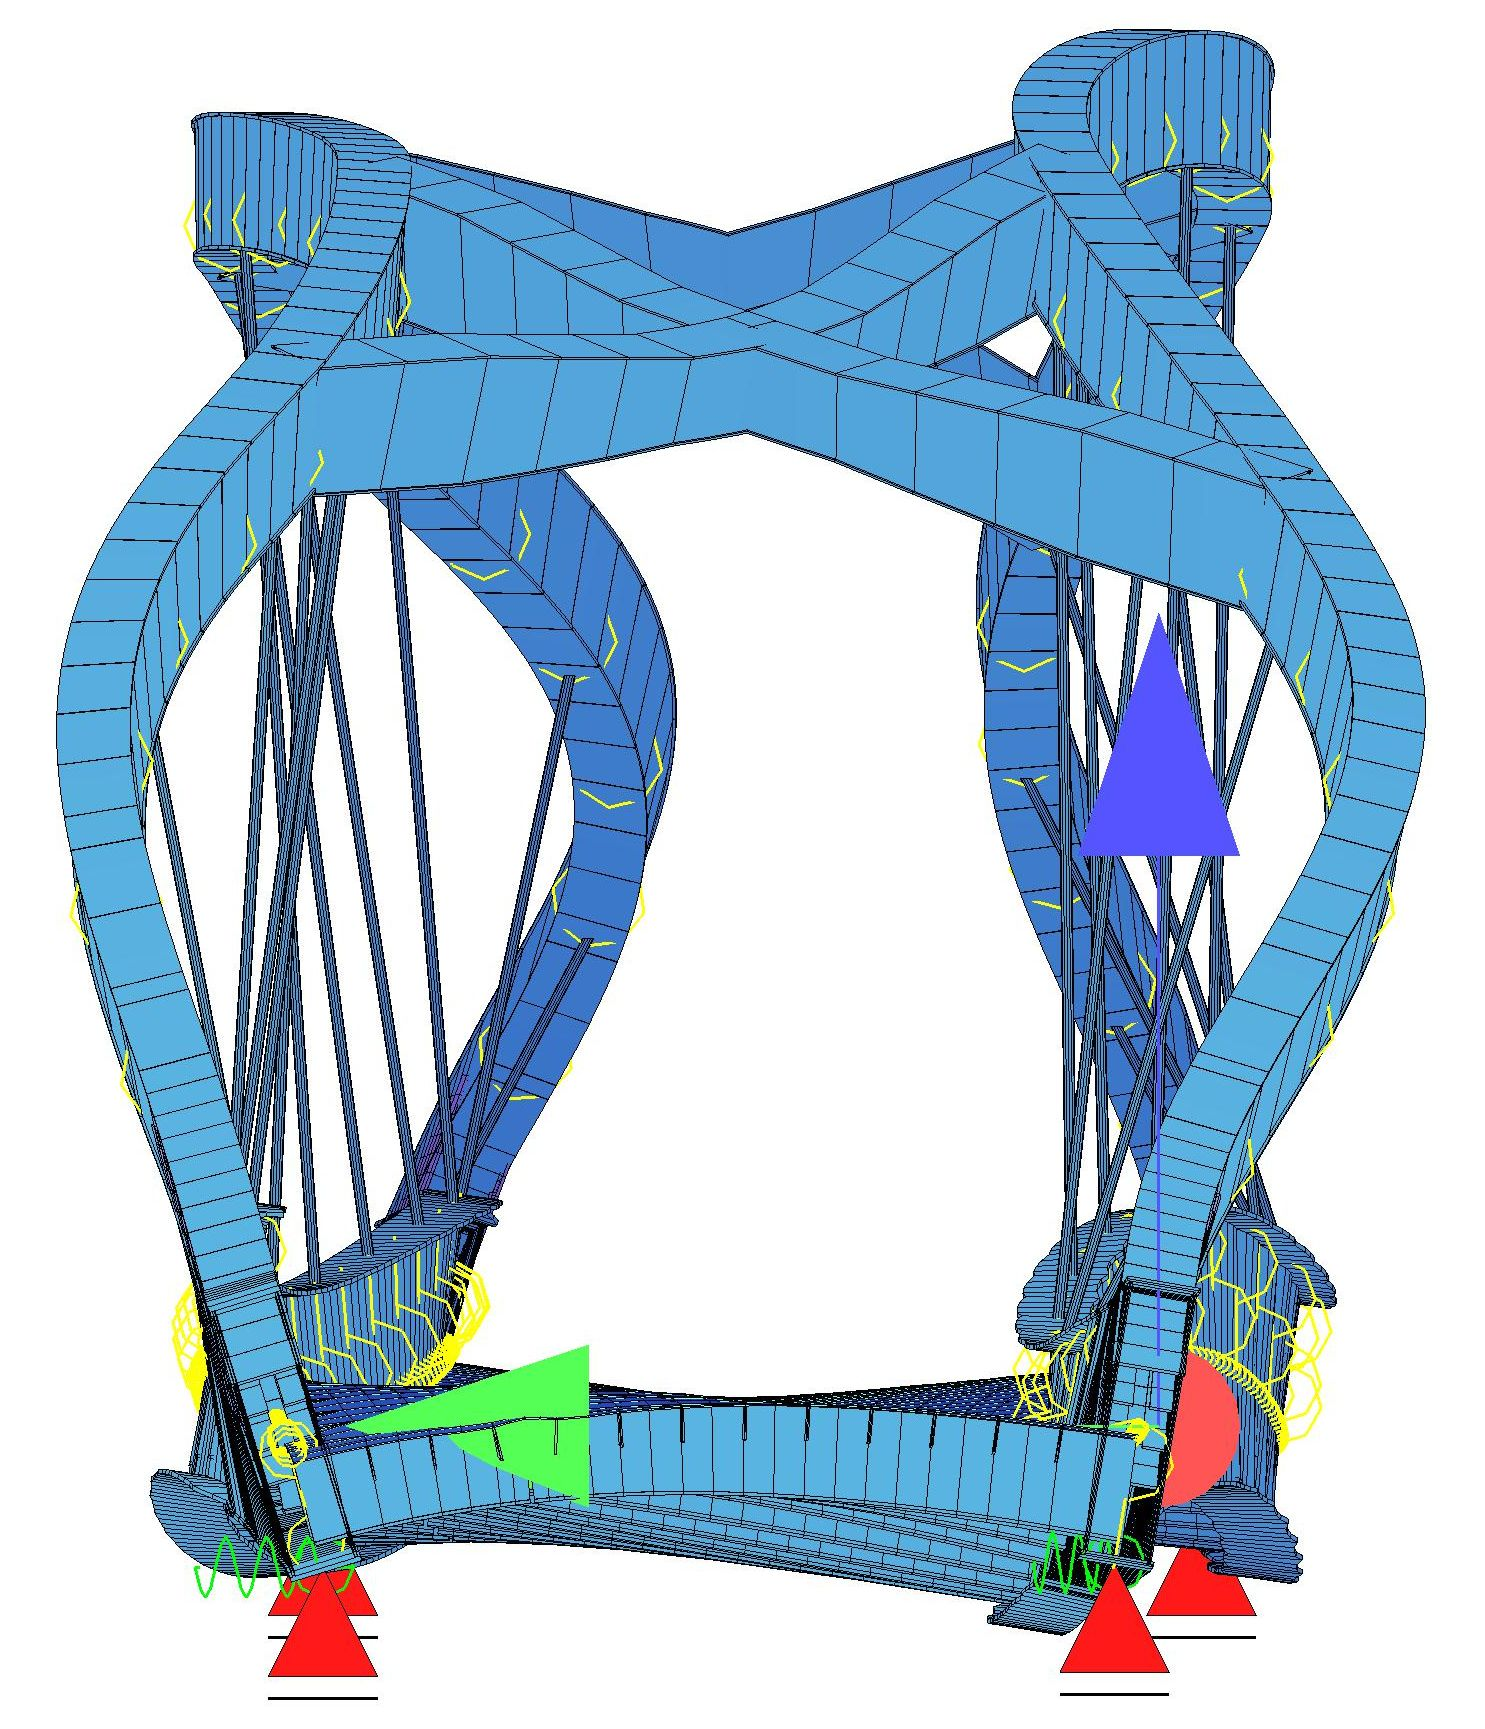
\includegraphics[height=0.12\textheight]{/WK2/model/mod_origin/f10f.jpg}%
				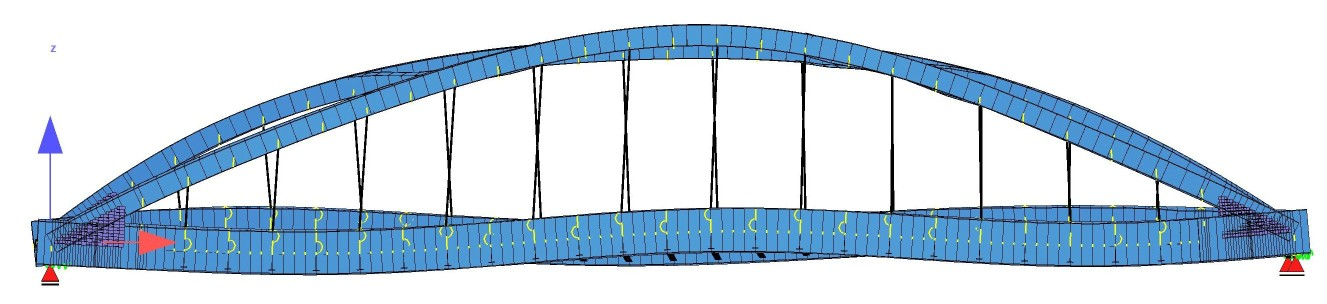
\includegraphics[width=0.7\textwidth]{/WK2/model/mod_origin/f10s.jpg}%
		\end{tabular}}\\
	\end{tabular}
	\caption{Postaci i częstotliwości drgań własnych wiaduktu WK2 - Model wstępny. Kont.}
	
\end{figure}

\section{Identyfikacja modalna wiaduktu WK2} \label{sect: identyfikacja_modalna_wk2}
Przed przystąpieniem do procesu optymalizacji układu statycznego dźwigara łukowego model należało skalibrować (p. \ref{sect:calibration_model}). Z uwagi na zakres planowanych analiz dynamicznych kluczowe jest, aby model w odpowiedni sposób odwzorowywał rzeczywistość w zakresie parametrów modalnych. Mając do dyspozycji rzeczywisty obiekt, zdecydowano o wykonaniu badań terenowych, które pozwolą na identyfikację częstotliwości i postaci drgań własnych oraz towarzyszącego im tłumienia. Obiekt jest w ciągłej eksploatacji. Z tych względów zdecydowano o wykorzystaniu Operacyjnej Analizy Modalnej do identyfikacji parametrów modalnych przęsła (p. \ref{sect:OMA}).

Przed przystąpieniem do badań przygotowano plan zawierający kluczowe punkty, bez których spełnienia badania mogą zakończyć się niepowodzeniem lub wyniki mogą być trudne w interpretacji. W pracy \cite{Brincker2015} autorzy sporządzili listę zaleceń, które należy wypełnić w trakcie przygotowań eksperymentu OMA. Podobne zalecenia w sformułowano w pracy \cite{Poprawa2018}. W kontekście założonych celów i przedmiotowego obiektu badawczego główne z nich to:
\begin{itemize}
\item opracowanie strategi prowadzenia badań i akwizycji danych,
\item uzgodnienia administracyjne - wstęp na obiekt i możliwość prowadzenia badań pod ruchem,
\item dobranie sprzętu pomiarowego.
\end{itemize}

Zarządca obiektu zezwolił na prowadzenie badań pod ruchem w towarzystwie sygnalisty. Średnie natężenie ruchu na obiekcie w trakcie badań to około 1 przejazd na 30 min. Wybór sprzętu pomiarowego ograniczał się do zastosowania posiadanego systemu do akwizycji przyspieszeń opisanego w punkcie \ref{sect: next_era_lab_test}. Najistotniejszym punktem przygotowania badań było opracowanie strategii badań. Według \cite{Brincker2015} plan badań OMA powinien zawierać następujące punkty:
\begin{itemize}
	\item sporządzoną siatkę pomiarową,
	\item kolejność ustawień czujników w seriach pomiarowych,
	\item określenie liczby osób potrzebnych do przeprowadzenia eksperymentu,
	\item zapewnienie bezpieczeństwa w trakcie badań,
	\item określenie parametrów akwizycji danych (częstotliwość próbkowania, długość pomiarów, liczba powtórzeń serii pomiarowych itd.)
\end{itemize}

\subsubsection{Wybór punktów pomiarowych} \label{sect:choose_measuremanet_locations}
Dostępny system pomiarowy składał się jedynie z dwóch akcelerometrów 3-osiowych i z dwóch czujników 1-osiowych.  Mając do dyspozycji ograniczoną liczbę jednocześnie mierzonych punktów przeprowadzono symulację najlepszego rozmieszczenia punktów pomiarowych na obiekcie. Przykłady metod pozwalających na optymalne rozmieszczenie punktów pomiarowych w analizach dynamicznych zaprezentowano w literaturze i najczęściej opierają się one na wyznaczeniu reprezentatywnego wskaźnika, dzięki któremu da się porównać różne ustawienia. Między innymi w \cite{Kammer1991,Papadopoulos1998} zaproponowano użycie Modalnej Energii Kinetycznej \teng{Modal Kinetic Energy}, w \cite{Udwadia1994} macierzy informacyjnej Fishera \teng{Fisher Information Matrix}, a w \cite{Penny1994,Allemang2003} macierzy MAC dla zestawu modów. W pracy \cite{Zhang2017} przedstawiono zwięzłe zestawienie powyższych metod i zaproponowano opcję optymalizującą lokalizację punktów pomiarowych przy wielu ustawieniach pomiarowych, zarówno dla punktów pomiarowych jak i punktów referencyjnych. Autorzy zwracają również uwagę, że przy wielu punktach pomiaru ścisła ocena wszystkich możliwych ustawień jest wymagająca obliczeniowo bądź niemożliwa. Z tego względu stosowane są algorytmy heurystyczne bądź meta-heurystyczne. 

W niniejszej pracy zastosowano metodę wykorzystującą kryterium MAC \parencite{Penny1994}. Podobne postępowanie przedstawiono w pracy \cite{Poprawa2018}. Polega ono na wyznaczeniu teoretycznych postaci drgań własnych z dostępnego modelu MES. Dla zbioru wszystkich możliwych położeń czujników odczytywane są przemieszczenia znormalizowane danej postaci drgań. Dalej, ze zbioru możliwych położeń wybierane są punkty, gdzie umieszczone mają zostać czujniki. Posiłkując się opisem postaci drgań w wybranych punktach tworzona jest macierz MAC. Każdą postać porównuje się ze wszystkimi innymi i z samą sobą. W ten sposób na przekątnej macierzy pojawiają się wartości równe 1 co oznacza oczywiste, idealne dopasowanie postaci według kryterium MAC. Poza przekątną, wartości MAC mieszczą się w przedziale 0 - 1. Celem analizy jest dobór punktów pomiarowych tak by poza przekątną wartości były możliwie małe. Przy małym dopasowaniu, postaci będą miały szanse być zidentyfikowane jednoznacznie przy mocno ograniczonej liczbie punktów pomiarowych i bliskim położeniu modów w dziedzinie częstotliwości. Dla każdego rozwiązania należy wyznaczyć wskaźnik, który pozwala ocenić zbiór punktów względem innych. Autorzy pracy \cite{Penny1994} zaproponowali w jednym z wariantów maksymalną wartość MAC wśród elementów poza przekątną macierzy oraz średnią kwadratową (RMS)\footnote{
	Średnią kwadratową wyznaczono zgodnie z definicją z równania: $x_{\text{RMS}}=\sqrt{\frac{x_1^2+x_2^2+x_3^2+\dots+x_n^2}{n}}$} 
ze wszystkich elementów powyżej przekątnej macierzy MAC. Im niższa wartość maksymalna i im niższa średnia kwadratowa tym lepiej.
\begin{figure}[hbt!]
	\centering
	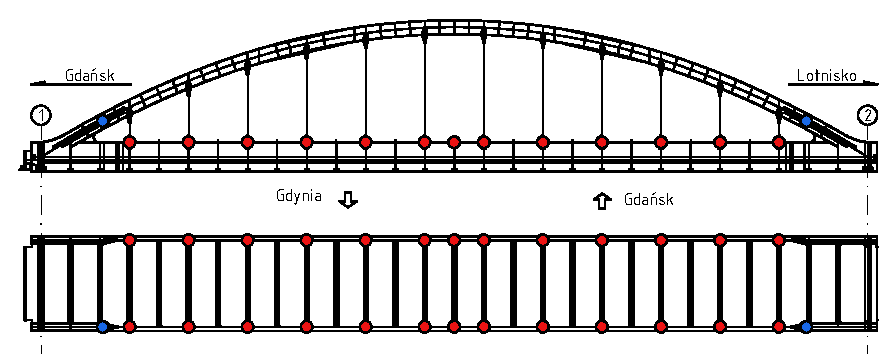
\includegraphics{/WK2/rysunki/punkty_pomiarowe_automac_croped.pdf}
	\captionsetup{justification=centering}
	\caption{Lokalizacje dozwolone przy doborze punktów pomiarowych}
	\label{fig: wk2_automac_points_all}
\end{figure}

Z uwagi na ograniczony czas dostępu do obiektu ustalono, że całość badań musi być zrealizowana w 3 ustawieniach dostępnych czujników. W przypadku wiaduktu, akcelerometry 3-osiowe potraktowano jako 2-osiowe. Odrzucono pomiar wzdłuż osi podłużnej jako nieistotny. W tej sytuacji jeden czujnik 2-osiowy posłużył jako punkt referencyjny mierzący drgania pionowe i poprzeczne. Pozostałe 4 punkty pomiarowe mogły być zmieniane w poszczególnych ustawieniach. Ostatecznie przy trzech ustawieniach możliwy był pomiar w 14 punktach pomiarowych $(6+4+4)$ w tym 10 na kierunku pionowym $Z$ i 4 na kierunku poprzecznym $Y$. Kolejnym koniecznym przy doborze siatki pomiarowej ograniczeniem było to, że dostęp do konstrukcji był możliwy jedynie z pomostu. Z uwagi na występowanie modów związanych głównie z bocznym ruchem łuków (Rys. \ref{fig: model_wk2_origin_mods}) narzucono, że 4 punkty pomiarowe $2Y$ i $2Z$ zostaną zamocowane bezpośrednio na łuku, tuż przy wezgłowiach. Uwzględniając powyższe założenia pozostało do dyspozycji 8 punktów pomiarowych $Z$ i 2 punkty pomiarowe $Y$. Punkty $Y$ są związane z $Z$ w ramach obudowy czujnika 2-osiowego, zaniechano więc doboru lokalizacji z uwagi na punkty $Y$ i skupiono się tylko na kierunku $Z$. Na rysunku \ref{fig: wk2_automac_points_all} kolorem czerwonym zaznaczono zbiór wszystkich dozwolonych do wyboru punktów. Kolorem niebieskim zaznaczono punkty zarezerwowane dla czujników mocowanych do łuku. Punków czerwonych jest 26 i należy z nich wybrać 8. Wykonano kombinację bez powtórzeń i uzyskano 1 562 275 zestawów lokalizacji czujników. Dla każdego zestawu wyznaczono macierz MAC uwzględniając 10 pierwszych modów z modelu MES, a następnie obliczono RMS i maksymalny element każdej macierzy. Zestawy posortowano względem każdego z tych wskaźników i wyniki przedstawiono graficznie na rysunku \ref{fig: wk2_automac_charts}. 
\begin{figure}[hbt!]
	\centering
	\captionsetup{justification=centering}
	\subfloat[Maksymalna wartość MAC wśród elementów poza przekątną macierzy]{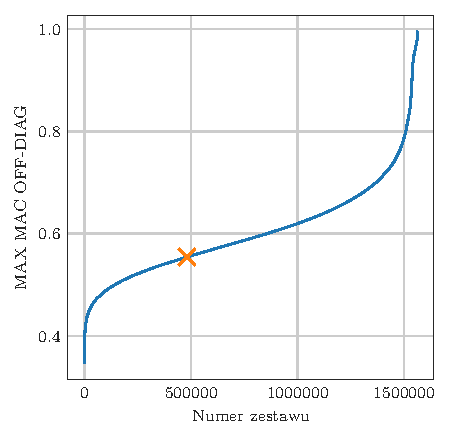
\includegraphics[]{/WK2/automac/max_mac.pdf}}% 
	\subfloat[RMS wszystkich elementów poza przekątną macierzy]{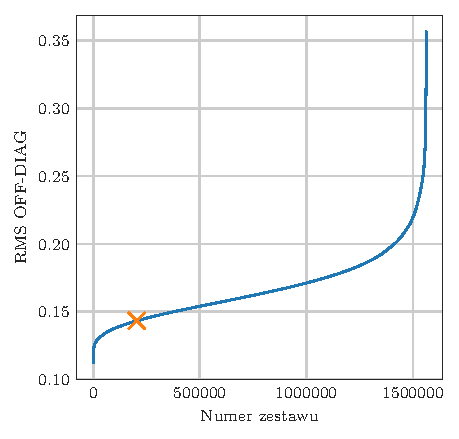
\includegraphics[]{/WK2/automac/rms.pdf}} 
	\captionsetup{justification=centering}
	\caption{Wskaźniki oceniające jakość wyboru zestawu punktów pomiarowych dla wszystkich analizowanych kombinacji}
	\label{fig: wk2_automac_charts}
\end{figure}
Logicznym wyborem punktów byłoby wzięcie pod uwagę ustawień charakteryzujących się minimalną wartością jednego z parametrów. Jednakże prowadząc badania terenowe należy brać pod uwagę czynniki takie jak ułożenie kabli, możliwości systemu pomiarowego do łączenia punktów pomiarowych czy przejście z kablami przez czynną linię kolejową na wiadukcie. Z tego powodu zaproponowano układ czujników intuicyjnie pozwalających na dobrą identyfikację modalną, a jednocześnie gwarantujący komfort w montażu i kontroli przez jedną osobę. Wybrane punkty pokazano na rysunku \ref{fig: wk2_automac_points_choosen}. Dla wybranego zestawu punktów wyznaczono macierz MAC (Rys. \ref{fig: wk2_automac_correlogram}) i wskaźniki: RMS i maksymalną wartość MAC. Wskaźniki zaznaczono na rysunku \ref{fig: wk2_automac_charts} pomarańczowym krzyżykiem, pokazując jakość dokonanego wyboru wśród wszystkich możliwych opcji. Na podstawie wartości RMS można stwierdzić, że narzucony wariant charakteryzuje się niską wartością parametru i jego dalsze optymalizowanie kosztem utrudnień w trakcie pomiarów, oceniono jako nieopłacalne. Należy również zaznaczyć, że wartość RMS elementów poza przekątną macierzy MAC mierzy jedynie średnią zależność wszystkich par wektorów. Nie uwzględnia wielkości amplitud poszczególnych modów w punktach i ich znaczenia na ostateczne zachowanie dynamiczne wiaduktu. W przedmiotowym przypadku zamocowano punkty pomiarowe w miejscach, gdzie kryterium RMS jest jednocześnie niskie (Rys. \ref{fig: wk2_automac_charts}) i przemieszczenia modalne dla głównych modów giętnych i skrętnych pomostu są bliskie ekstremalnym (Rys. \ref{fig: model_wk2_origin_mods}).


\begin{figure}[hbt!]
	\centering
	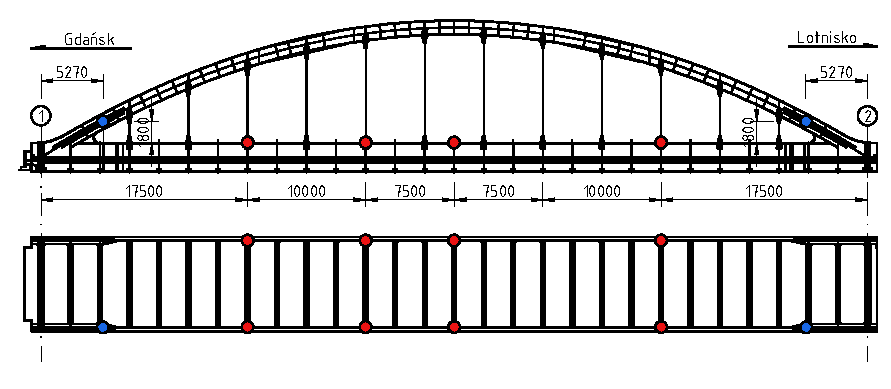
\includegraphics{/WK2/rysunki/punkty_pomiarowe_punkty_pomiarowe_croped.pdf}
	\captionsetup{justification=centering}
	\caption{Wybrane do badań punkty pomiaru przyspieszeń pionowych}
	\label{fig: wk2_automac_points_choosen}
\end{figure}


\begin{figure}[hbt!]
	\centering
	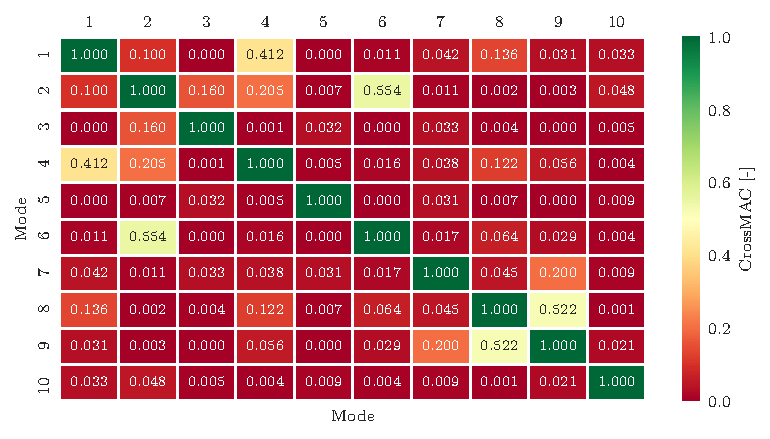
\includegraphics[width=\textwidth]{WK2/automac/correlogram_0.pdf}
	\captionsetup{justification=centering}
	\caption{Macierz MAC dla pierwszych dziesięciu wektorów postaci drgań własnych, odczytanych z modelu dla wybranych punktów pomiarowych}
	\label{fig: wk2_automac_correlogram}
\end{figure}


\subsubsection{Parametry akwizycji danych}
Przed przystąpieniem do badań wyznaczono podstawowe parametry pozwalające na przeprowadzenie poprawnego eksperymentu OMA. Posługując się formułami (\ref{eq: oma_min_sampling}) i (\ref{eq: oma_min_time_series}) określono minimalną częstotliwość próbkowania jako $f_{s,min}=2.4\cdot8=19.2\,\text{Hz}$ i minimalny czas prowadzenia pomiarów w jednym ustawieniu jako $T_{min}=\frac{10}{0.005\cdot1.4}=1429\,\text{s}=23.8\,\text{min}$. Ostatecznie zdecydowano o prowadzeniu pomiarów ze znacznym nadpróbkowaniem o częstotliwości $f_s=300\,\text{Hz}$ i w seriach czasowych 20 - 30 min, w zależności od rozkładu jazdy pojazdów po obiekcie.


\subsubsection{Przebieg badań}
Badania na obiekcie przeprowadzone zostały w dniu 17 czerwca 2019 r. Wykorzystano zestaw pomiarowy opisany w rozdziale \ref{sect: next_era_lab_test}. Zestaw w trakcie badań pokazano na rysunku \ref{fig: wk2_foto_aparatura}. Pomiary wykonano zgodnie z planem. Akwizycję danych podzielono na 3 ustawienia. Akwizycja danych w każdym ustawieniu wynosiła od 20 do 30 min. Punkty pomiarowe w poszczególnych ustawieniach oznaczono na rysunku \ref{fig: wk2_automac_points_choosen}. Warunki atmosferyczne były stabilne, stwierdzono brak odczuwalnych podmuchów wiatru i silne operowanie słońca.

\begin{figure}[hbt!]
	\centering
	\subfloat[System akwizycji danych: komputer i wzmacniacz pomiarowy HBM PMX]{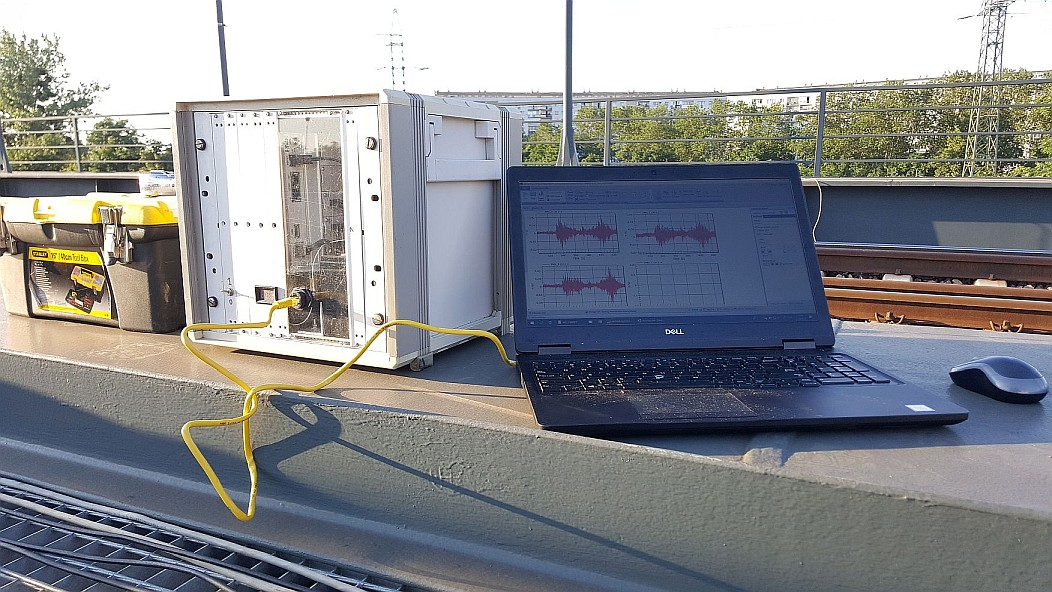
\includegraphics[width=0.48\linewidth]{/WK2/zdjecia/system_pomiarowy.jpg}} \quad 
	\subfloat[3 osiowy akcelerometr piezorezystancyjny]{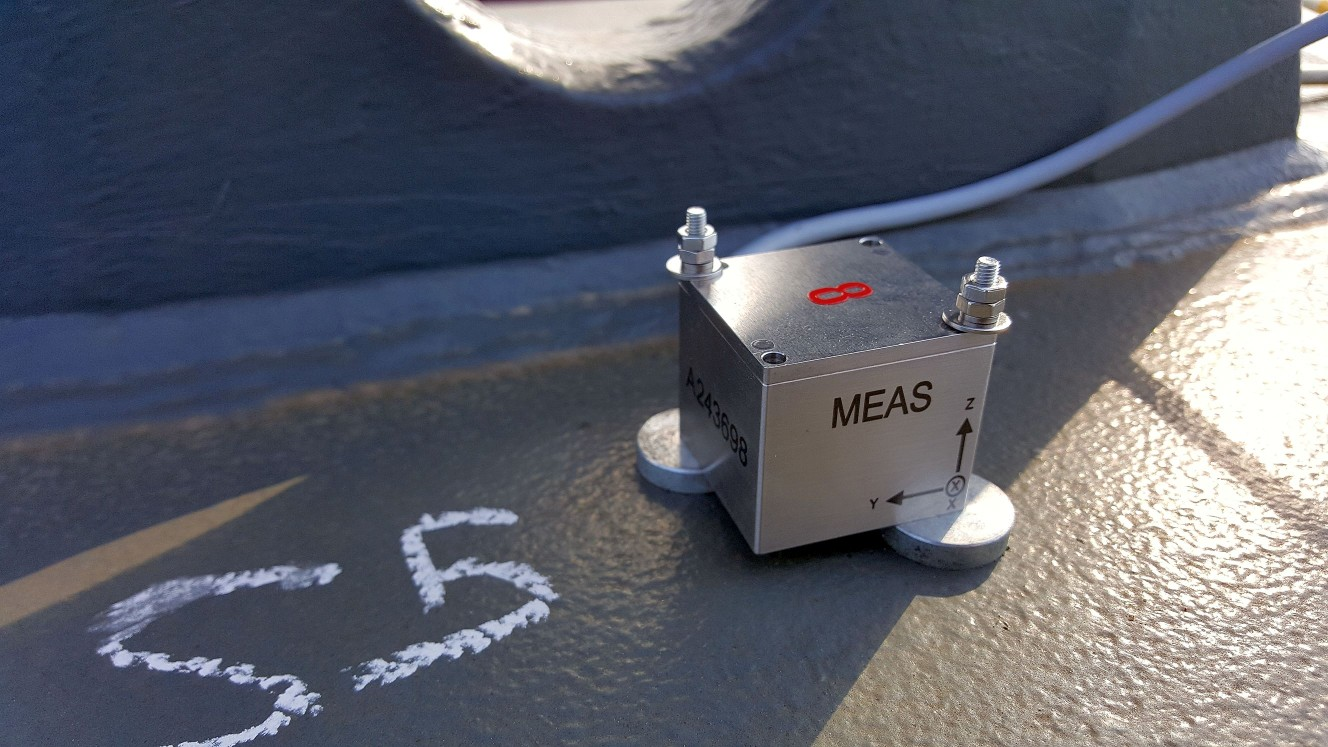
\includegraphics[width=0.48\linewidth]{/WK2/zdjecia/czujnik_3_osie.jpg}} 
	\captionsetup{justification=centering}
	\caption{System pomiarowy użyty do identyfikacji modalnej wiaduktu WK2}
	\label{fig: wk2_foto_aparatura}
\end{figure}

\subsubsection{Środki obciążeniowe}
W trakcie badań na obiekcie odbywał się standardowy dla PKM ruch pociągów pasażerskich. Pomiary prowadzono pomiędzy przejazdami po obiekcie spełniając w ten sposób lepiej kryterium stacjonarności. Masa taboru kolejowego poruszającego się po obiekcie stanowi znaczący ułamek masy całkowitej wiaduktu WK-2 i mogłaby wpłynąć na zmianę parametrów modalnych konstrukcji. Pomiędzy przejazdami, w asyście sygnalisty eksperymentator przemieszczał się biegając i podskakując po obiekcie (Rys. \ref{fig: wk2_foto_obciazenia}. Oddziaływanie jednego człowieka na obiekcie odznaczało się wyraźnymi amplitudami przyspieszeń przęsła. 
\begin{figure}[hbt!]
	\centering
	%\subfloat[]{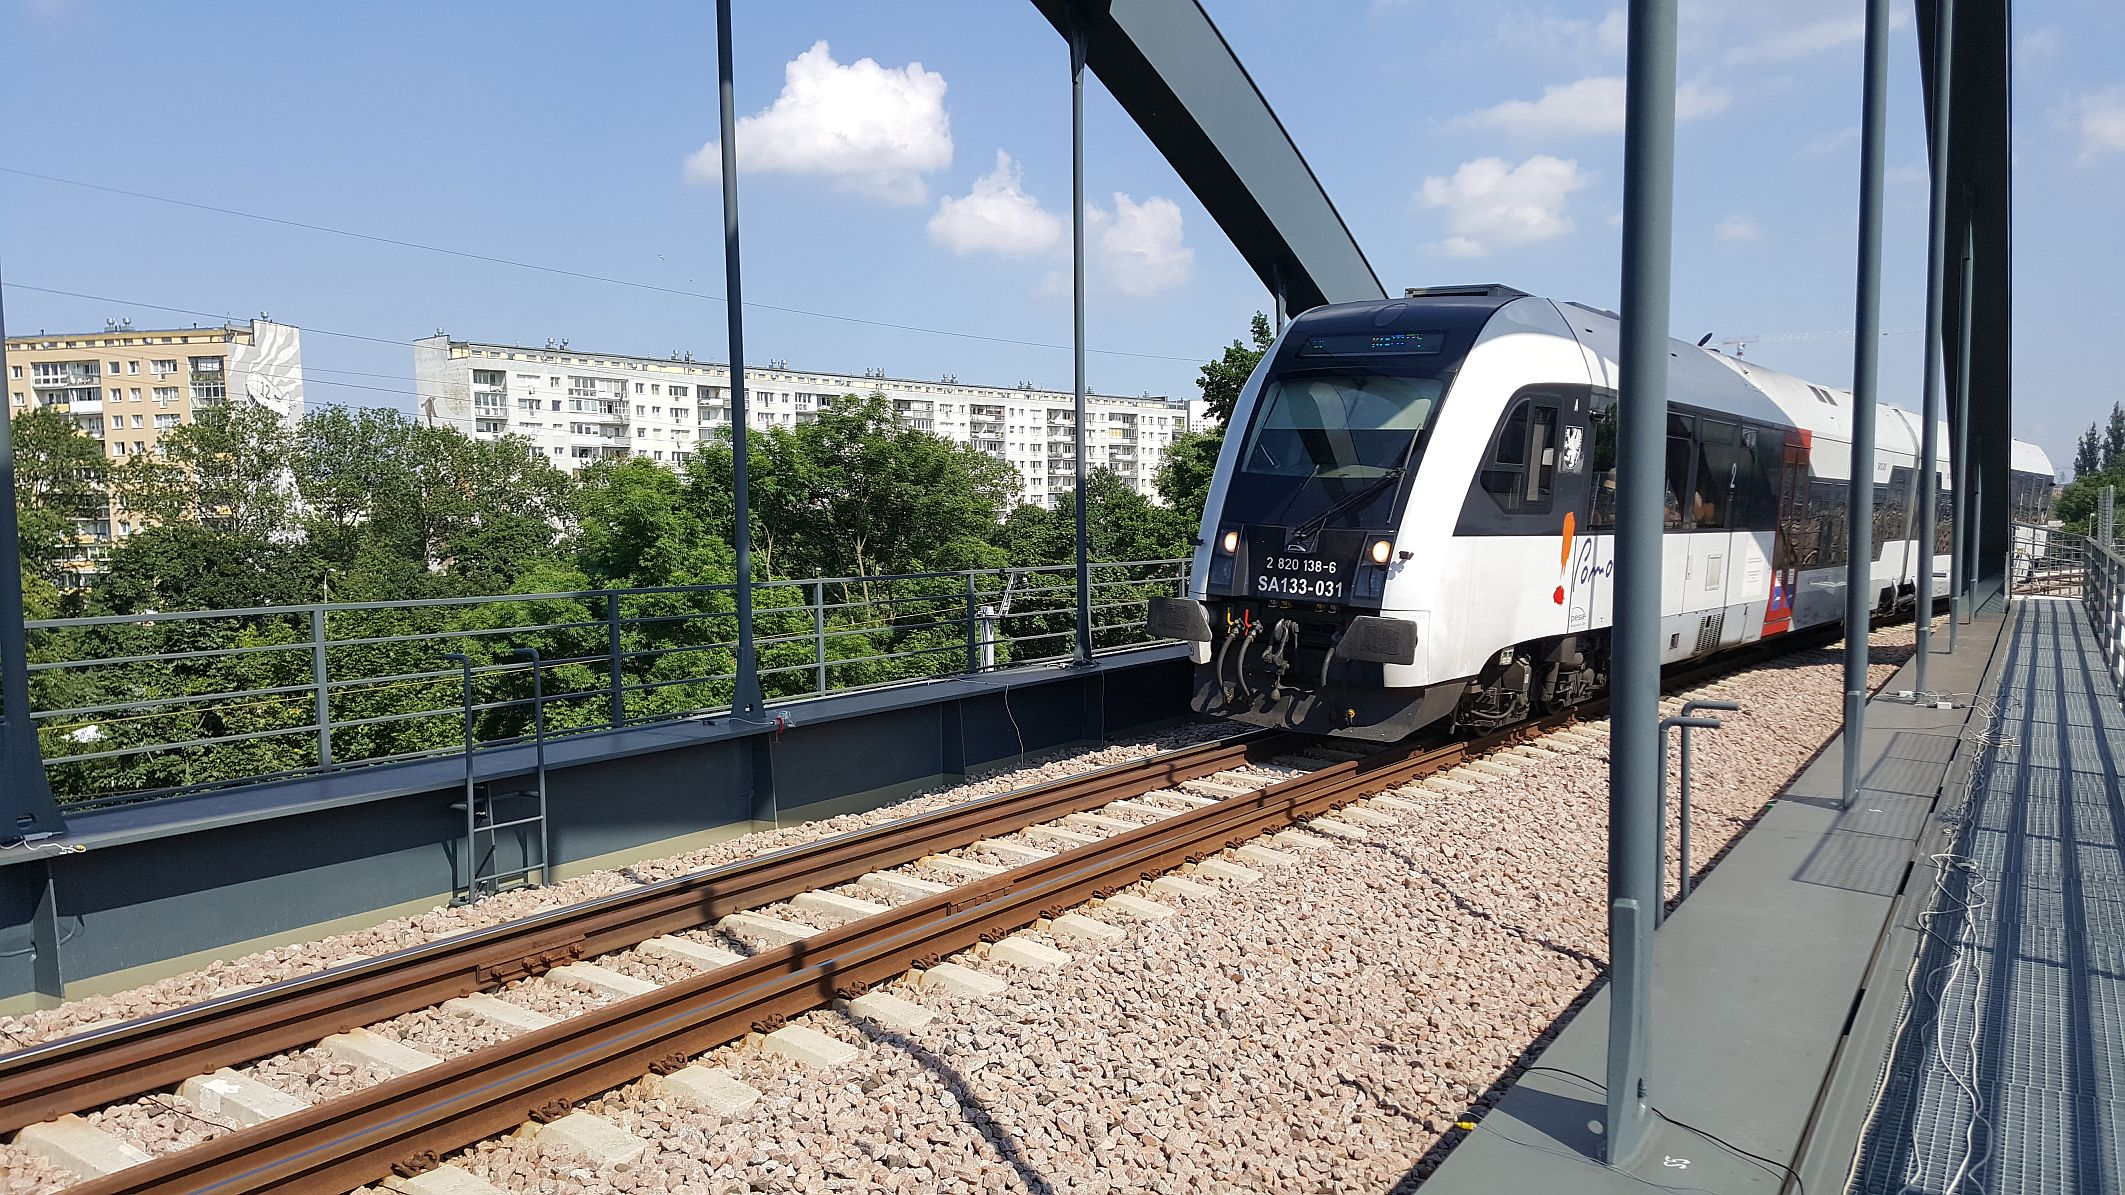
\includegraphics[height=0.15\textheight]{/WK2/zdjecia/pojazd_na.jpg}} \quad
	%\subfloat[]{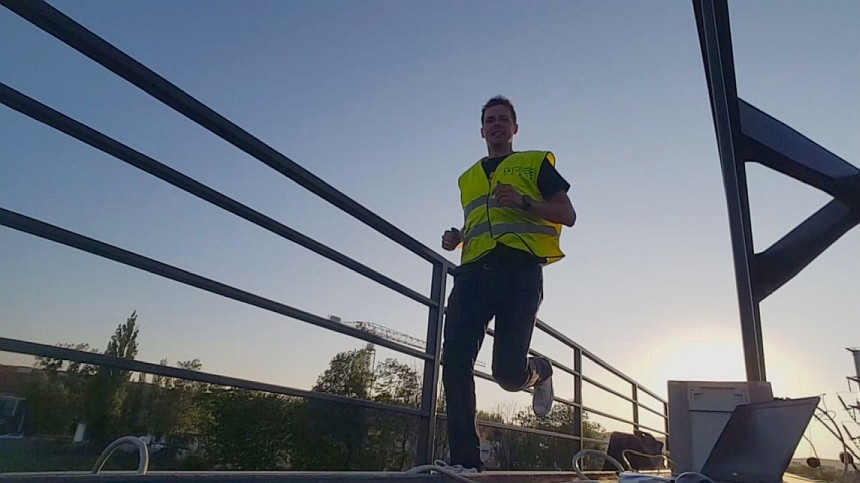
\includegraphics[height=0.15\textheight]{/WK2/zdjecia/eksperymentator.jpg}}
	\subfloat[Pojazd SA133-031 wjeżdżający na obiekt]{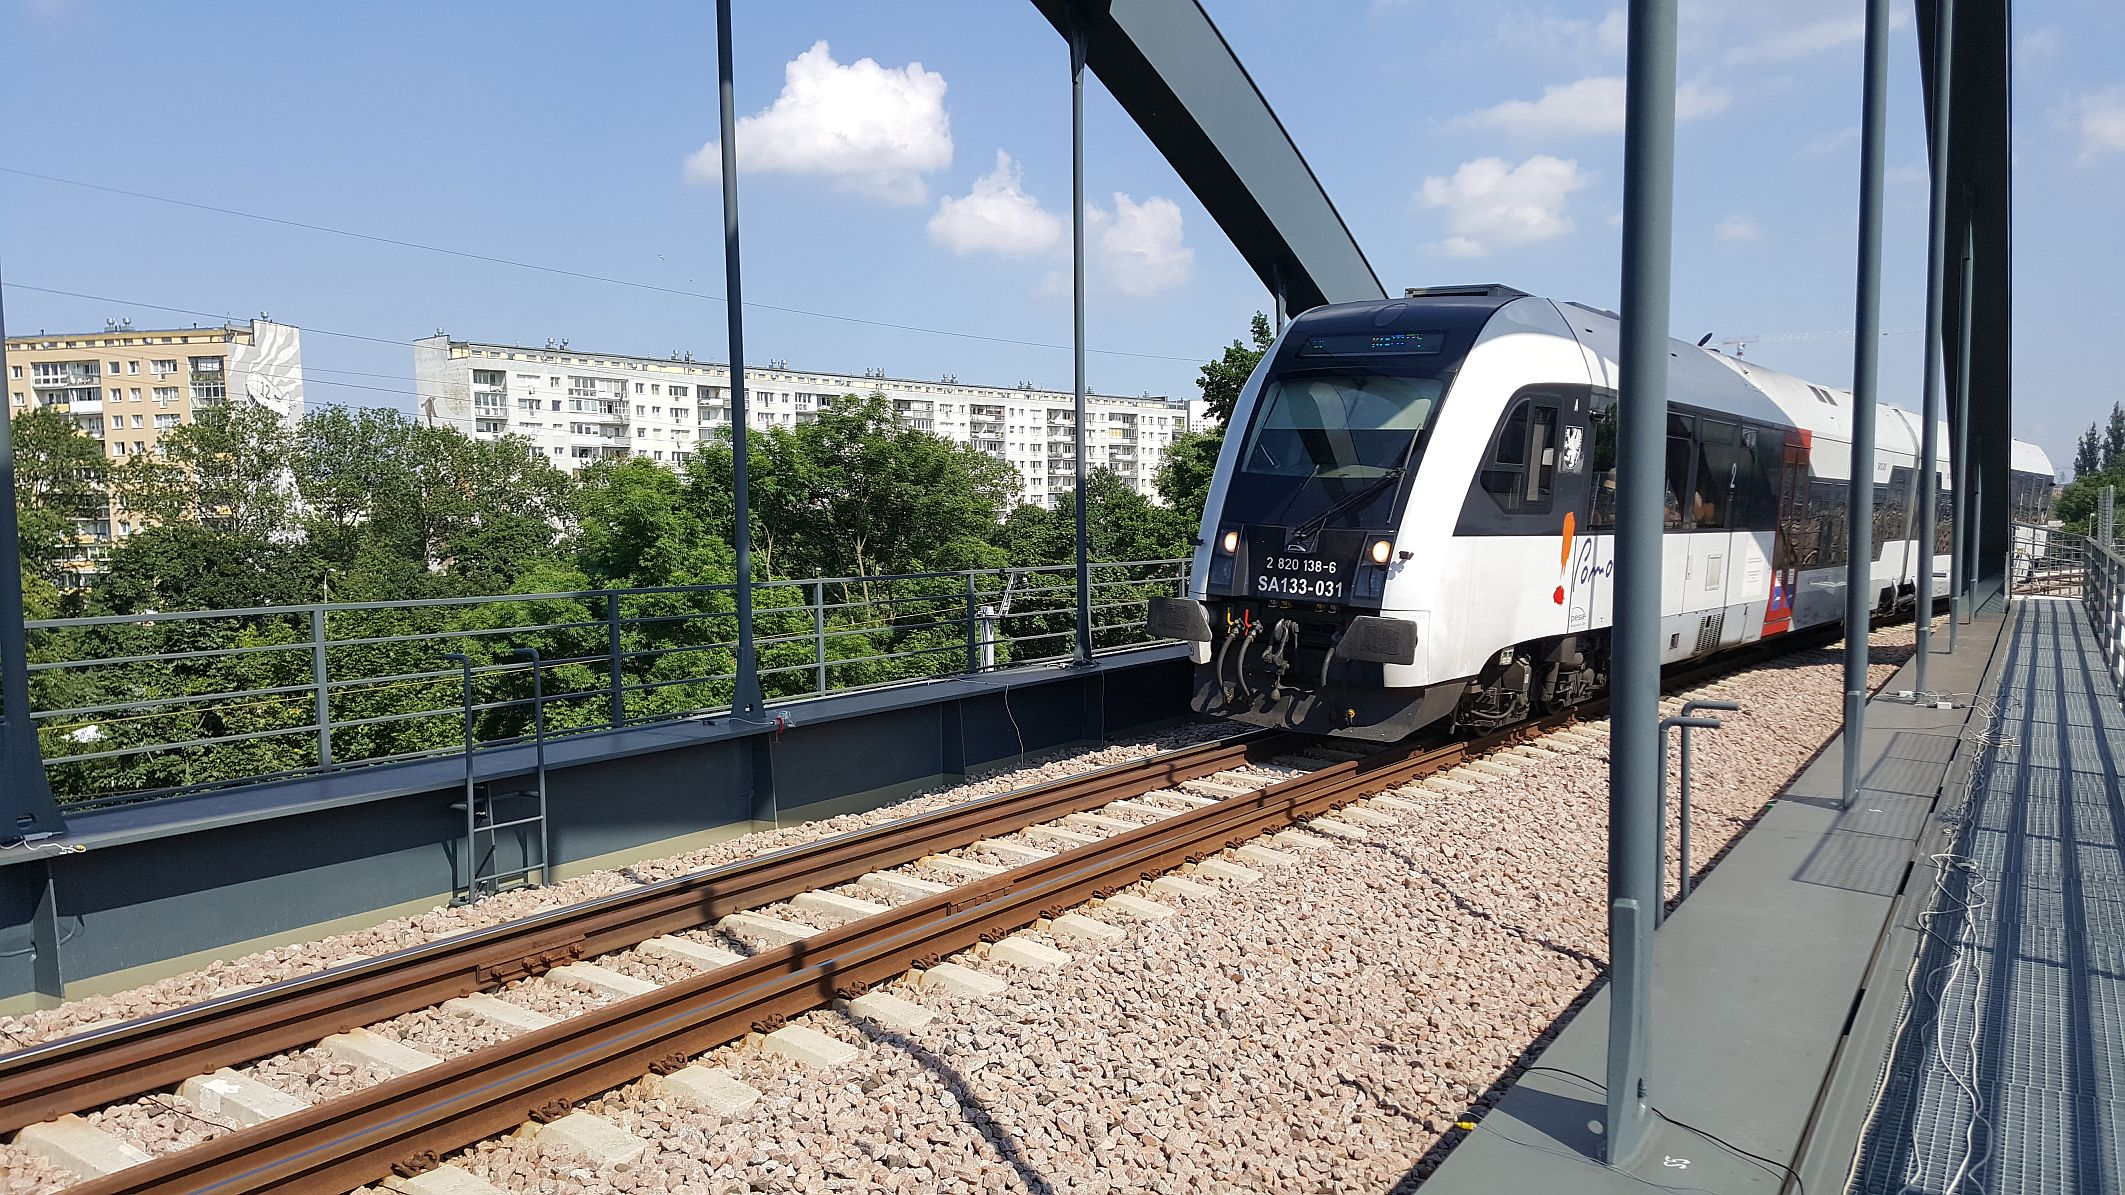
\includegraphics[width=0.48\textwidth]{/WK2/zdjecia/pojazd_na.jpg}} \quad
	\subfloat[Eksperymentator w trakcie obciążania]{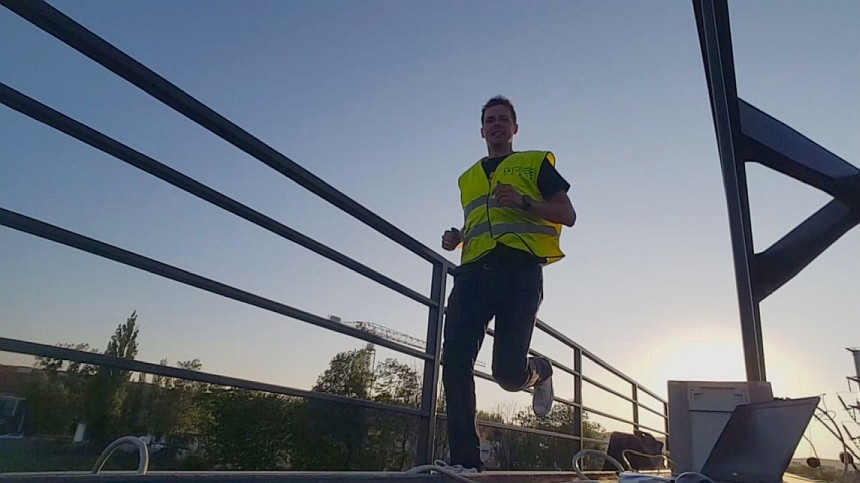
\includegraphics[width=0.48\textwidth]{/WK2/zdjecia/eksperymentator.jpg}}
	\captionsetup{justification=centering}
	\caption{Obciążenia w trakcie badań obiektu WK-2}
	\label{fig: wk2_foto_obciazenia}
\end{figure}

Zauważono również inne, pomniejsze oddziaływania środowiskowe. Pod obiektem odbywał się ruch w ciągu magistralnej linii kolejowej nr 202. W odległości około 150 m od wiaduktu, niemal równolegle przebiega główna arteria Gdańska - aleja Grunwaldzka, na której ciągu dnia panuje stały, znaczny ruch samochodowy. W podobnej odległości od obiektu panowały prace budowlane z wykorzystaniem ciężkiego sprzętu. Niestety nie stwierdzono praktycznie żadnych podmuchów wiatru.



\subsubsection{Analiza i rezultaty badań}
Zarejestrowane sygnały poddano analizie OMA metodą NExT-ERA. Użyto autorskiego programu opisano w punkcie \ref{sect: OMA_application}. W procesie iteracyjnym przyjęto parametry metody pozwalające uzyskać stabilne rozwiązania. Uwzględniając wyniki z teoretycznej analizy modalnej (Rys. \ref{fig: model_wk2_origin_mods}), stwierdzono że niektóre częstotliwości drgań własnych są położone bardzo blisko siebie w dziedzinie częstotliwości. Autor pracy \cite{Caicedo2011} w takiej sytuacji proponuje obniżenie częstotliwości próbkowania sygnału. Zabieg ten zwiększa szanse na zidentyfikowanie blisko położonych modów przez uwzględnienie w analizie mniejszego, całkowitego zakresu częstotliwości. Zastosowano resampling do próbkowania 30Hz. Szerokość okna FFT przy obliczaniu funkcji korelacji przyjęto równą 1024 próbki. Wybrane okno przy zmniejszonej częstotliwości próbkowania pozwoliło uzyskać funkcje korelacji o długości około 17 s. Wymiary macierzy Hankela przyjęto o wymiarach $r=110$ i $s=150$. Uwzględniono w ten sposób w macierzy Hankela niespełna 9 s odpowiedzi impulsowej danej funkcjami korelacji. Taki czas pozwala na uwzględnienie kilkunastu okresów drgań modu o najniższej częstotliwości. Na rysunku \ref{fig: wk2_research_stabdiags} przestawiono diagramy stabilizacyjne metody w wersji filtrowanej i niefiltrowanej dla rzędu maksymalnego równego $n=150$. Przy tworzeniu diagramów zastosowano następujące kryteria poprawności rozwiązania:
\begin{itemize}
	\item maksymalna różnica częstotliwości (\ref{eq: stabdiag_crit_freq}): $\Delta f \le 0.005$,
	\item maksymalny tłumienia (\ref{eq: stabdiag_crit_ksi}): $\Delta \xi \le 0.03$,
	\item minimalne kryterium MAC i MPC (\ref{eq: stabdiag_crit_MPC_MAC}): $\text{MPC}\ge 0.95$ i  $\text{MAC}\ge 0.95$
\end{itemize}


 Zidentyfikowano 10 pierwszych modów o częstotliwościach mniejszych niż 8 Hz. Pomimo zidentyfikowania również modów o wyższych częstotliwościach dalsze rozważania ograniczono do pierwszych dziesięciu. Z praktycznego punktu widzenia, dla obiektów mostowych jedynie kilka najniższych modów ma znaczący wpływ na odpowiedź dynamiczną konstrukcji, ale w ramach pracy badawczej poświęcono uwagę większej liczbie modów. Charakterystyki zidentyfikowanych modów przedstawiono na wykresach \ref{fig: wk2_research_mods1} i w tabeli \ref{tab: wk2_ident_mods}. Pierwszych 10 zidentyfikowanych częstotliwości drgań własnych jest zbliżonych do wyznaczonych teoretycznie ze wstępnego modelu MES (Rys. \ref{fig: model_wk2_origin_mods}). Wartości Logarytmicznego Dekrementu Tłumienia wahają się od 1.3\% do 7.7\%. Biorąc pod uwagę, że Wiadukt WK2 jest konstrukcją stalową z korytem wypełnionym tłuczniem, rezultaty te nie wzbudzają zastrzeżeń. Zidentyfikowane postaci drgań pozwalają odróżnić od siebie mody, ale wyraźnie cierpią z uwagi na zbyt słabe odwzorowanie postaci. Postaci związane z drganiami poprzecznymi łuków identyfikowane są praktycznie przez węzły zlokalizowane blisko wezgłowii i przez przemieszczenia pomostu realizujące się przez połączenie łuków ze ściągiem za pomocą wieszaków. Pomimo wspólnej normalizacji przemieszczeń modalnych pionowych i poprzecznych, wartości dla punków na łukach nie są znacznie większe niż przemieszczenia pomostu. Utrudnia to jednoznaczne powiązanie właściwych postaci bliskich sobie modów z postaciami uzyskanymi w modelu teoretycznym. Gdyby to było możliwe, zamocowanie punktów pomiarowych na łuku, w większej liczbie i w wyższych partiach mogłoby istotnie ułatwić identyfikację postaci i dalsze działania związane z kalibracją modelu. Podsumowując, identyfikację uznano za udaną i pozwalającą na ocenę konstrukcji i kalibrację modelu numerycznego. Jednakże istnieją uzasadnione uwagi co do liczby i rozmieszczenia czujników, które warto wyeliminować, ale wynikały z obiektywnych przeszkód w trakcie badań.

\begin{figure}[hbt!]
	\centering
	\subfloat[Diagram niefiltrowany]{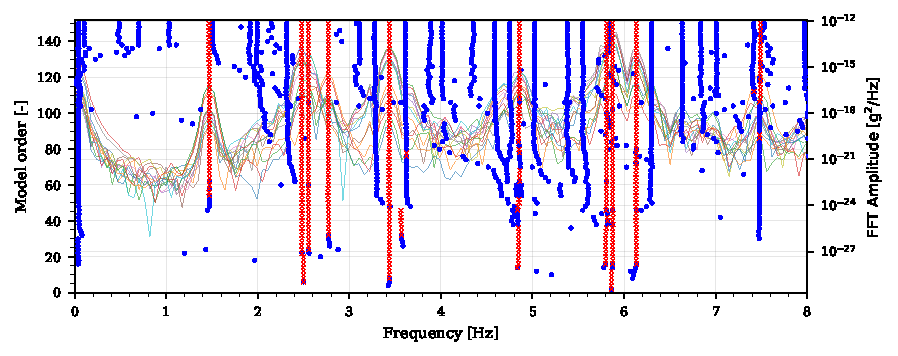
\includegraphics[]{WK2/ident/fig_stab_diagram_nonfiltr.pdf}}\\
	\subfloat[Diagram filtrowany]{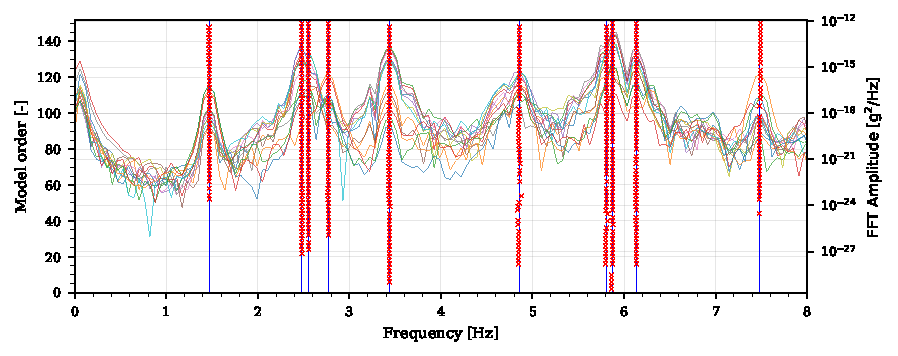
\includegraphics[]{WK2/ident/fig_stab_diagram_filtr.pdf}}
	\captionsetup{justification=centering}
	\caption{Diagramy stabilizacyjne metody NExT-ERA w badaniach wiaduktu WK2}
	\label{fig: wk2_research_stabdiags}
\end{figure}

\begin{table}[hbt!]
	\caption{Zidentyfikowane charakterystyki modalne wiaduktu WK2}
	\label{tab: wk2_ident_mods}
	\footnotesize
	\setlength\tabcolsep{0pt}
	\begin{tabular}{@{} p{0.25\linewidth} *{10}{P{0.075\linewidth}} @{}}
	\toprule
	\textbf{Mod}  & \textbf{1} & \textbf{2} & \textbf{3} & \textbf{4} & \textbf{5} & \textbf{6} & \textbf{7} & \textbf{8} & \textbf{9} & \textbf{10} \\ \midrule
	\textbf{Częstotliwość {[}Hz{]}}   & 1.468          & 2.481          & 2.551          & 2.769          & 3.435          & 4.853          & 5.809          & 5.874          & 6.132          & 7.483           \\ \midrule
	\textbf{Liczba tłumienia {[}-{]}} & 0.007          & 0.009          & 0.006          & 0.011          & 0.012          & 0.012          & 0.005          & 0.005          & 0.002          & 0.004           \\ \midrule
	\textbf{LDT {[}-{]}}              & 0.043          & 0.053          & 0.037          & 0.070          & 0.077          & 0.077          & 0.028          & 0.031          & 0.013          & 0.024           \\ \bottomrule
\end{tabular}
\end{table}





\begin{figure}[p]
	\centering
	\begin{tabular}[c]{c}
	\subfloat[Mod 1, $f_1=1.468\, \text{Hz}$]{\label{fig: wk2_research_mod01}%
			\begin{tabular}[b]{c c c}
				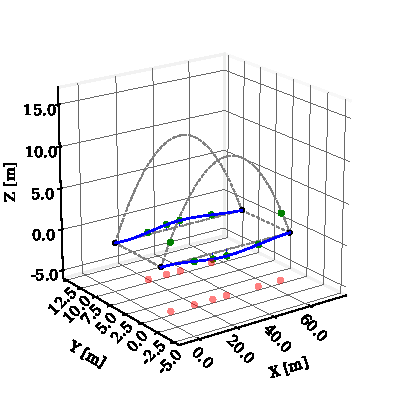
\includegraphics[height=0.20\textheight,trim=0 0 0 25,clip]{/wk2/ident/mods/fig_mod_11_time_20_08_21.pdf}%
				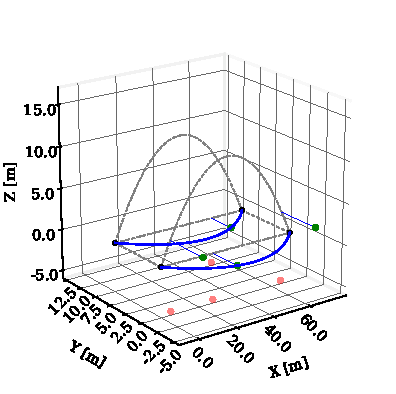
\includegraphics[height=0.20\textheight,trim=0 0 0 25,clip]{/wk2/ident/mods/fig_mod_11_time_13_58_03.pdf}%
				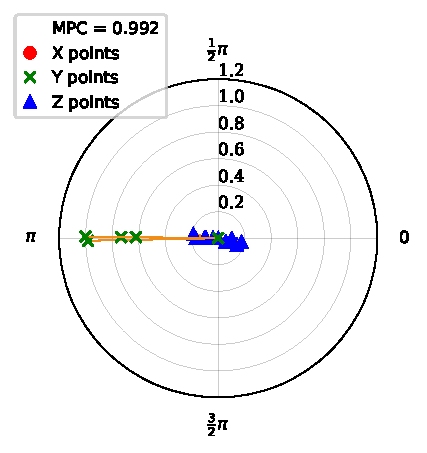
\includegraphics[height=0.20\textheight]{/wk2/ident/mods/fig_polar_mod_11_time_13_59_19.pdf}%
		\end{tabular}}\\
	\subfloat[Mod 2, $f_2=2.481\,\text{Hz}$]{\label{fig: wk2_research_mod02}%
	\begin{tabular}[b]{c c c}
		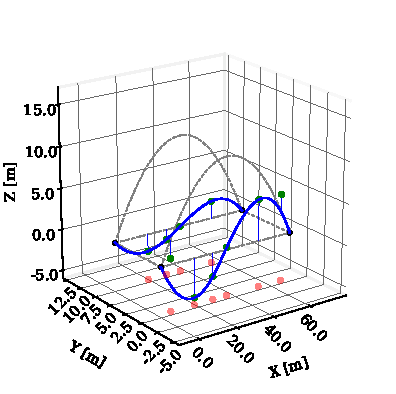
\includegraphics[height=0.20\textheight,trim=0 0 0 25,clip]{/wk2/ident/mods/fig_mod_23_time_20_09_19.pdf}%
		\includegraphics[height=0.20\textheight,trim=0 0 0 25,clip]{/wk2/ident/mods/fig_mod_23_time_20_09_26.pdf}%
		\includegraphics[height=0.20\textheight]{/wk2/ident/mods/fig_polar_mod_23_time_16_57_54.pdf}%
\end{tabular}}\\
	\subfloat[Mod 3, $f_3=2.551\, \text{Hz}$]{\label{fig: wk2_research_mod03}%
	\begin{tabular}[b]{c c c}
		\includegraphics[height=0.20\textheight,trim=0 0 0 25,clip]{/wk2/ident/mods/fig_mod_25_time_20_09_56.pdf}%
		\includegraphics[height=0.20\textheight,trim=0 0 0 25,clip]{/wk2/ident/mods/fig_mod_25_time_20_10_13.pdf}%
		\includegraphics[height=0.20\textheight]{/wk2/ident/mods/fig_polar_mod_25_time_16_58_42.pdf}%
\end{tabular}}\\
	\subfloat[Mod 4, $f_4=2.769\, \text{Hz}$]{\label{fig: wk2_research_mod04}%
	\begin{tabular}[b]{c c c}
		\includegraphics[height=0.20\textheight,trim=0 0 0 25,clip]{/wk2/ident/mods/fig_mod_27_time_20_10_31.pdf}%
		\includegraphics[height=0.20\textheight,trim=0 0 0 25,clip]{/wk2/ident/mods/fig_mod_27_time_14_00_02.pdf}%
		\includegraphics[height=0.20\textheight]{/wk2/ident/mods/fig_polar_mod_27_time_14_00_19.pdf}%
\end{tabular}}\\

	\end{tabular}
\caption{Zidentyfikowane charakterystyki modalne wiaduktu WK2}
\label{fig: wk2_research_mods1}
\end{figure}


\begin{figure}[p]\ContinuedFloat
	\centering
	\begin{tabular}[c]{c}
	\subfloat[Mod 5, $f_5=3.435\, \text{Hz}$]{\label{fig: wk2_research_mod05}%
	\begin{tabular}[b]{c c c}
		\includegraphics[height=0.20\textheight,trim=0 0 0 25,clip]{/wk2/ident/mods/fig_mod_33_time_20_11_02.pdf}%
		\includegraphics[height=0.20\textheight,trim=0 0 0 25,clip]{/wk2/ident/mods/fig_mod_33_time_20_11_12.pdf}%
		\includegraphics[height=0.20\textheight]{/wk2/ident/mods/fig_polar_mod_33_time_17_00_05.pdf}%
\end{tabular}}\\

	\subfloat[Mod 6, $f_6=4.853\, \text{Hz}$]{\label{fig: wk2_research_mod06}%
	\begin{tabular}[b]{c c c}
		\includegraphics[height=0.20\textheight,trim=0 0 0 25,clip]{/wk2/ident/mods/fig_mod_47_time_20_11_28.pdf}%
		\includegraphics[height=0.20\textheight,trim=0 0 0 25,clip]{/wk2/ident/mods/fig_mod_47_time_20_11_53.pdf}%
		\includegraphics[height=0.20\textheight]{/wk2/ident/mods/fig_polar_mod_47_time_17_00_46.pdf}%
\end{tabular}}\\
	\subfloat[Mod 7, $f_7=5.809\, \text{Hz}$]{\label{fig: wk2_research_mod07}%
	\begin{tabular}[b]{c c c}
		\includegraphics[height=0.20\textheight,trim=0 0 0 25,clip]{/wk2/ident/mods/fig_mod_57_time_20_12_12.pdf}%
		\includegraphics[height=0.20\textheight,trim=0 0 0 25,clip]{/wk2/ident/mods/fig_mod_57_time_20_12_20.pdf}%
		\includegraphics[height=0.20\textheight]{/wk2/ident/mods/fig_polar_mod_57_time_17_01_27.pdf}%
\end{tabular}}\\
	\subfloat[Mod 8, $f_8=5.874\, \text{Hz}$]{\label{fig: wk2_research_mod08}%
	\begin{tabular}[b]{c c c}
		\includegraphics[height=0.20\textheight,trim=0 0 0 25,clip]{/wk2/ident/mods/fig_mod_59_time_20_12_37.pdf}%
		\includegraphics[height=0.20\textheight,trim=0 0 0 25,clip]{/wk2/ident/mods/fig_mod_59_time_20_12_48.pdf}%
		\includegraphics[height=0.20\textheight]{/wk2/ident/mods/fig_polar_mod_59_time_17_02_08.pdf}%
\end{tabular}}\\
	\end{tabular}
\caption{Zidentyfikowane charakterystyki modalne wiaduktu WK2 kont.}
\label{fig: wk2_research_mods2}
\end{figure}


\begin{figure}[H]\ContinuedFloat
	\centering
	\begin{tabular}[c]{c}
	\subfloat[Mod 9, $f_9=6.132\, \text{Hz}$]{\label{fig: wk2_research_mod09}%
	\begin{tabular}[b]{c c c}
		\includegraphics[height=0.20\textheight,trim=0 0 0 25,clip]{/wk2/ident/mods/fig_mod_61_time_20_13_07.pdf}%
		\includegraphics[height=0.20\textheight,trim=0 0 0 25,clip]{/wk2/ident/mods/fig_mod_61_time_20_13_32.pdf}%
		\includegraphics[height=0.20\textheight]{/wk2/ident/mods/fig_polar_mod_61_time_17_17_06.pdf}%
\end{tabular}}\\
	\subfloat[Mod 10, $f_{10}=7.483\, \text{Hz}$]{\label{fig: wk2_research_mod10}%
	\begin{tabular}[b]{c c c}
		\includegraphics[height=0.20\textheight,trim=0 0 0 25,clip]{/wk2/ident/mods/fig_mod_75_time_20_13_51.pdf}%
		\includegraphics[height=0.20\textheight,trim=0 0 0 25,clip]{/wk2/ident/mods/fig_mod_75_time_14_01_31.pdf}%
		\includegraphics[height=0.20\textheight]{/wk2/ident/mods/fig_polar_mod_75_time_14_01_40.pdf}%
\end{tabular}}\\



	\end{tabular}
	\caption{Zidentyfikowane charakterystyki modalne wiaduktu WK2 kont.}
	\label{fig: wk2_research_mods3}
\end{figure}

\section{Kalibracja modelu numerycznego z wykorzystaniem PSO} \label{sect:wk2_calibration}
Stworzony wstępny model numeryczny powstał z wykorzystaniem założeń projektowych. Wykonana identyfikacja parametrów dynamicznych i przeprowadzone badania odbiorcze pod próbnym obciążeniem dostarczyły szereg informacji o obiekcie w jego rzeczywistej formie. Dzięki dostarczonym danym możliwe jest przeprowadzenie kalibracji, która sprawi, że model będzie wierniej odzwierciedlał rzeczywistą konstrukcję. Kalibracja opierać będzie się na następujących danych wyjściowych:
\begin{itemize}
	\item przemieszczenia statyczne konstrukcji pod próbnym obciążeniem: 2 ustawienia po 6 punktów pomiarowych umiejscowionych na dźwigarach-ściągach,
	\item zidentyfikowane parametry modalne konstrukcji: 10 pierwszych częstotliwości i postaci drgań własnych oraz odpowiadające im tłumienia modalne. Postaci drgań opisane zostały za pomocą 14 współrzędnych modalnych (p. \ref{sect:choose_measuremanet_locations})
\end{itemize}
Przemieszczenia pozyskane z próbnych obciążeń statycznych pozwoli skalibrować głównie sztywność poszczególnych elementów konstrukcji. Z kolei parametry modalne, jako wartości odnoszące się do zachowania dynamicznego, związane są ze sztywnością konstrukcji oraz masą konstrukcyjną i niekonstrukcyjną.

Obiekty łukowe, podobnie jak kratownicowe są relatywnie złożonymi obiektami. Na ich charakterystykę dynamiczną wpływa wiele czynników, które mniej lub bardziej potrafią wpłynąć na parametry modalne. Różni to je od statycznie nieskomplikowanych obiektów belkowych czy płytowych oraz od dużych obiektów wiszących i podwieszonych gdzie rozwiązania i szczegóły konstrukcyjne nie wpływają aż tak istotnie na globalne zachowanie dynamiczne konstrukcji. Dla łukowego wiaduktu WK2 wyodrębniono 22 czynniki, które będą podlegać modyfikacji w trakcie kalibracji. Podzielono je na trzy rodzaje: sztywności elementów konstrukcyjnych, sztywności warunków brzegowych oraz masy konstrukcyjne i niekonstrukcyjne. Poniżej zestawiono symbole zmiennych wraz z ich opisem:
\begin{itemize}
	\item Sztywności elementów konstrukcyjnych:
	\begin{itemize}
		\item S1 - łuku,
		\item S2 - ściągu,
		\item S3 - poprzecznic,
		\item S4 - żeber płyty ortotropowej,
		\item S5 - blachy płyty ortotropowej,
		\item S6 - stężeń górnych,
		\item S7 - wieszaków,
		\item S8 - elementów stanowiących usztywniających wezgłowie łuku.
	\end{itemize}
	\item Sztywność warunków brzegowych (Rys. \ref{fig:boudary_conditions_stiff_bearings}):
	\begin{itemize}
		\item S21 - Oś 2, podpora A, kierunek X,
		\item S22 - Oś 1, podpora A, kierunek Y,
		\item S23 - Oś 1, podpora B, kierunek X,
		\item S24 - Oś 2, podpora B, kierunek X,
		\item S25 - Oś 1, podpora A, kierunek X,
		\item S26 - Oś 2, podpora A, kierunek Y,
		\item S27 - Oś 1, podpora B, kierunek Y,
		\item S28 - Oś 2, podpora B, kierunek Y.
	\end{itemize}
	\item Masa elementów konstrukcyjnych i niekonstrukcyjnych:
	\begin{itemize}
		\item M1 - łuku,
		\item M2 - ściągu,
		\item M3 - tłucznia - część wzdłuż osi toru,
		\item M4 - tłucznia - część równomiernie rozłożona,
		\item M5 - pomostu roboczego,
		\item M6 - stężeń górnych.
	\end{itemize}
\end{itemize}

\begin{figure}[hbt!]
	\centering
	\includegraphics[width=\textwidth]{WK2/rysunki/lozyska_sprezyny_kalibracja.pdf}
	\captionsetup{justification=centering}
	\caption{Projektowany schemat łożyskowania i rozmieszczenia podpór sprężystych, modyfikowanych w procesie kalibracji}
	\label{fig:boudary_conditions_stiff_bearings}
\end{figure}
Na bazie doświadczeń można stwierdzić, że liczba ujętych w rozważaniach zmiennych jest zbyt duża. Niektóre z wymienionych elementów intuicyjnie nie wpływają znacząco na globalne charakterystyki modalne konstrukcji. Dotyczy to między innymi sztywności elementów pomostu czy warunków brzegowych, w przypadku gdzie w rzeczywistości zastosowano precyzyjnie wykonane łożyska mostowe. W klasycznych metodach kalibracji analiza wrażliwości pozwoliłaby wykluczyć takie zmienne. Jednakże w niniejszej pracy pozostawiono zwiększoną liczbę zmiennych, żeby mieć pełną kontrolę nad modelem oraz uwidocznić zalety zastosowanej metody kalibracji.

Kalibrację modelu postanowiono potraktować jako problem optymalizacji. Problem zdefiniowano standardowo przez wybór funkcji celu, parametrów i zmiennych projektowych oraz ograniczeń. Funkcją celu jest miara dopasowania modelu do konstrukcji rzeczywistej pod względem odpowiedzi statycznej i charakterystyk dynamicznych. Parametry projektowe definiują model numeryczny poddawany kalibracji i zostały przyjęte na podstawie dokumentacji powykonawczej. Zmienne projektowe stanowią wymienione wyżej 22 parametry: sztywności elementów konstrukcji, warunków brzegowych i masy znajdujące się na obiekcie. Jako metodę optymalizacji globalnej przyjęto metodę roju cząstek PSO w wersji wielokryterialnej. 

\subsection{Funkcja celu}
Funkcja celu w zdefiniowanym problemie w założeniu powinna być miarą dopasowania modelu do konstrukcji rzeczywistej. W literaturze do kalibracji najczęściej stosowane są jednokryterialne algorytmy, w których miara dopasowania wyrażona jest jedną wartością liczbową. Wynikowa wartość jest więc najczęściej liniową kombinacją kryteriów dopasowania. W idealnym przypadku gdzie wszystkie kryteria zbiegają do najlepszego rozwiązania jednocześnie byłoby to w zupełności wystarczające podejście. Jednakże w rzeczywistości każde kryterium obarczone jest niedokładnościami. Błędy te wynikają z uproszczonej formy modelu numerycznego oraz z błędów pomiaru i procesu identyfikacji. Obecnie nie jest możliwe potraktowanie każdego najmniejszego elementu modelu jako zmiennej, ponieważ wymagałoby to ogromniej liczby zmiennych. W efekcie nie wszystkie kryteria dopasowania osiągają minimalna wartość dla jednego rozwiązania. Chcąc uniknąć narzucania skali ważności (wag) na poszczególne funkcje celu, optymalizację wykonano w wariancie wielokryterialnym. Zbiorem funkcji celu, z których każda jest minimalizowana i opisuje dopasowanie modelu do obiektu jest wektor $\vect{F}=[f_{freq},f_{disp},f_{MAC}]$. Na wartość funkcji $f_{freq}$ wpływ ma $N$ pierwszych częstotliwości drgań własnych modelu $f_i^n$ i odpowiadających, zidentyfikowanych na konstrukcji rzeczywistej $f_i^r$. Wyznaczana jest ona następująco:
\begin{equation} \label{eq:wk2_calib_f_freq}
f_{freq}=\sum_{i=1}^{N} (f_i^n - f_i^r)^2
\end{equation}
Funkcja celu $f_{disp}$ związana jest z przemieszczeniami uzyskiwanymi pod działaniem obciążenia statycznego. W rozważanym przypadku wykorzystano pomiar wykonany w trakcie próbnego obciążenia. Dla dwóch ustawień, po sześć punktów pomiarowych w każdym, porównano przemieszczenia pionowe zmierzone na konstrukcji rzeczywistej $d_i^r$ z wyznaczonymi w modelu numerycznym $d_i^n$. Wartość funkcji celu związanej z przemieszczeniami konstrukcji sformułowano jako wartość bezwzględną sumy różnic:
\begin{equation} \label{eq:wk2_calib_f_disp}
	f_{disp}=\sum_{i=1}^{12} |d_i^n - d_i^r|
\end{equation}
Ostatnia funkcja celu jest miarą dopasowania pierwszych $N$ postaci drgań własnych zidentyfikowanych na konstrukcji $\phi_i^r$ oraz wyznaczonych w modelu $\phi_i^n$. Do liczbowego porównania postaci użyto kryterium MAC. Wartość funkcji $f_{MAC}$ opisano następującym równaniem:
\begin{equation} \label{eq:wk2_calib_f_mass}
	f_{MAC}=\sum_{i=1}^{N} (1-\text{MAC}(\vect{\phi}_i^n, \vect{\phi}_i^r))^2
\end{equation}
gdzie $\text{MAC}(\cdot)$ oznacza kryterium MAC dwóch wektorów. Zasadniczo kryterium MAC dwóch wektorów powinno być maksymalizowane. Wszakże, dla idealnego dopasowania wektorów równe jest jedności, a dla zupełnego braku dopasowania - zeru. Jednakże, znając wartość maksymalną kryterium $\text{MAC}=1$ i stosując odejmowanie, przemianowano naturalnie maksymalizowaną funkcję celu na minimalizowaną. Dzięki temu wszystkie funkcje celu będą podlegać minimalizacji, co nie jest wymagane, ale uprasza interpretację wyników oraz zmniejsza stopień komplikacji algorytmu obliczeniowego.

\subsection{Zmienne projektowe}
Zmienne projektowe w procesie kalibracji przedstawiono w punkcie \ref{sect:wk2_calibration}. Pomimo, że niektóre zmiene odnoszą się do sztywności elementów konstrukcyjnych i ich masy, po zbudowaniu modelu numerycznego nie ulegał on modyfikacjom strukturalnym w procesie optymalizacji. Wszystkie zmienne były sterowane za pomocą mnożników nakładanych na sztywności i masy zamodelowanych elementów. Bazowe sztywności elementów i masy wynikają z modelu i przyjęto je na podstawie dokumentacji projektowej. Z kolei sztywności podpór sprężystych początkowo ustawiono jako stosunkowo sztywne, o stałej sprężystości równej $k=1\text{E}6\text{kN/m}$. 

Ograniczenia dla zmiennych projektowych stanowią wartości skrajne, podyktowane doświadczeniem i zdrowym rozsądkiem. Przykładowe niepewności dla różnych elementów modelu numerycznego przedstawiono w tabeli \ref{table:uncertainitesModel}. W tabelach \ref{tab:calibration_stiffness} - \ref{tab:calibration_mass} przedstawiono wszystkie zmienne projektowe (mnożniki wartości bazowych) oraz ich zakresy dopuszczalne. Szacując wartość możliwej odchyłki zmiennej wzięto pod uwagę typ elementu wykorzystanego w modelowaniu, ilość detali konstrukcyjnych pomijanych w modelu, możliwe niedokładności przy wykonaniu rzeczywistej konstrukcji oraz dokładność opisu elementu w dokumentacji projektowej. Przyjęte wartości skrajne można uznać za zawyżone (lub zaniżone), ale dzięki temu rozwiązania optymalne nie powinny być zlokalizowane blisko granicy zakresu dopuszczalnego. Zmniejsza to liczbę wymuszonych zmian położenia cząstek w trakcie optymalizacji (p. \ref{sect:pso_def}).

\begin{table}[hbt!]
	\caption{Zakres dopuszczalnych zmian sztywności elementów konstrukcyjnych}
	\label{tab:calibration_stiffness}
	\footnotesize
	\setlength\tabcolsep{0pt}
\begin{tabular}{@{}p{0.1\linewidth} p{0.05\linewidth} *8{P{0.10625\linewidth}}@{}}
	\toprule
	\multicolumn{2}{l}{\textbf{Element}}    & Łuk  & Ściąg & Poprzecz. & Żebra & Płyta & Stężenia & Wieszak & Wezgłowie \\ \midrule
	\multicolumn{2}{l}{\textbf{Oznaczenie}} & S1   & S2    & S3           & S4    & S5    & S6       & S7      & S8        \\ \midrule
	\multirow{2}{*}{\textbf{Zakres}}  & min & 0.85 & 0.85  & 0.85         & 0.8   & 0.85  & 0.7      & 0.9     & 1.0       \\ \cmidrule(){2-10} 
	& max & 1.15 & 1.15  & 1.15         & 1.2   & 1.15  & 1.3      & 1.1     & 6         \\ \bottomrule
\end{tabular}
\end{table}

\begin{table}[hbt!]

	\caption{Zakresy dopuszczalnych zmian sztywności warunków brzegowych}
	\centering
	\label{tab:calibration_supports}
	\footnotesize
	\setlength\tabcolsep{0pt}
	\begin{tabular}{@{}p{0.1\linewidth} p{0.05\linewidth} *8{P{0.10625\linewidth}}@{}}
		\toprule
		\multicolumn{2}{l}{\textbf{Podpora}}    & 2AX               & 1AY               & 1BX               & 2BX               & 1AX               & 2AY               & 1BY               & 2BY               \\ \midrule
		\multicolumn{2}{l}{\textbf{Oznaczenie}} & S21               & S22               & S23               & S24               & S25               & S26               & S27               & S28               \\ \midrule
		\multirow{2}{*}{\textbf{Zakres}}  & min & $1\mathrm{E}{-8}$ & $1\mathrm{E}{-8}$ & $1\mathrm{E}{-8}$ & $1\mathrm{E}{-8}$ & $1\mathrm{E}{-8}$ & $1\mathrm{E}{-8}$ & $1\mathrm{E}{-8}$ & $1\mathrm{E}{-8}$ \\ \cmidrule(){2-10} 
		& max & $1\mathrm{E}{3}$  & $1\mathrm{E}{3}$  & $1\mathrm{E}{3}$  & $1\mathrm{E}{3}$  & $1\mathrm{E}{3}$  & $1\mathrm{E}{3}$  & $1\mathrm{E}{3}$  & $1\mathrm{E}{3}$  \\ \bottomrule
	\end{tabular}
\end{table}



\begin{table}[hbt!]
	\caption{Zakresy dopuszczalnych zmian mass konstrukcyjnych i niekonstrukcyjnych}
	\label{tab:calibration_mass}
	\footnotesize
	\setlength\tabcolsep{0pt}
\begin{tabular}{@{}p{0.1\linewidth} p{0.05\linewidth} *6{P{0.1417\linewidth}}@{}}
	\toprule
	\multicolumn{2}{l}{\textbf{Element}}    & Łuk & Ściąg & Tłuczeń 1 & Tłuczeń 2 & Pomost & Stężenia \\ \midrule 
	\multicolumn{2}{l}{\textbf{Oznaczenie}} & M1  & M2    & M3        & M4        & M5     & M6       \\ \midrule
	\multirow{2}{*}{\textbf{Zakres}}  & min & 0.9 & 0.9   & 0.5       & 0.3       & 0.7    & 0.8      \\ \cmidrule(){2-8} 
	& max & 1.1 & 1.1   & 0.8       & 0.8       & 1.3    & 1.2      \\ \bottomrule
\end{tabular}
\end{table}



\subsection{Algorytm kalibracji}
Zaproponowane rozwiązanie kalibracji opiera się na podziale całego procesu na dwa obszary obliczeń. Pierwszy związany jest z wykorzystaniem komercyjnego oprogramowania MES SOFiSTiK, drugi to autorskie oprogramowanie umożliwiające optymalizację rojem cząstek. Oba obszary były połączone i zarządzane przez algorytm zapisany w języku Python.

\subsubsection{Analizy statyczna i modalna}
Przed przystąpieniem do optymalizacji, model numeryczny przęsła (Rys. \ref{fig: model_wk2_visualization}) przystosowano do kalibracji. Bazę danych zawierającą model MES powielono, aby stanowiła kopię zapasową w trakcie obliczeń. Do zdefiniowania obliczeń użyto program do preprocessingu tekstowego TEDDY i zapisano w nim wymagane w procesie kalibracji analizy i modyfikacje modelu. Uruchomienie instrukcji z pliku tekstowego wywoływało następujące obliczenia wykonywane przez moduł ASE \parencite{AG2018}:
\begin{itemize}
	\item analizę statyczną pod obciążeniem dwóch ustawień próbnego obciążenia,
	\item analizę statyczną pod obciążeniem od wszystkich dodatkowych, nieujętych w modelu detali konstrukcyjnych i wyposażenia obiektu,
	\item teoretyczną analizę modalną wyznaczającą 10 pierwszych postaci drgań własnych, przy dodaniu mas od wszystkich obciążeń stałych nieujętych w ciężarze własnym modelu konstrukcji.
\end{itemize}
W każdej z analiz zastosowane zostały mnożniki sztywności i mas o wartościach zmiennych projektowych rozpatrywanego rozwiązania. Uruchomienie następowało w odpowiednim momencie z poziomu programu optymalizacyjnego.

\subsubsection{Optymalizacja}
Jedną z cech algorytmów metaheurystycznych jest to, że są bardzo uniwersalne. Przystosowanie zapisanego w języku programowania algorytmu do danego problemu optymalizacji zazwyczaj nie wymaga wielu modyfikacji. W kalibracji modelu wykorzystano algorytm optymalizacji wielokryterialnej rojem cząstek MOPSO (\ref{sect:MOPSO_algorithm}). Współczynniki sterujące prędkością roju przyjęto jak w domyślnej wersji algorytmu: $\theta=0.7968$, $\alpha=1.4962$ oraz $\beta=1.4962$. Populację stanowił zbiór 70 cząstek, wygenerowanych w przestrzeni rozwiązań za pomocą sekwencji Haltona. Zastosowano topologię GBEST zapewniającą pełną wymianę informacji między cząstkami o najlepszym rozwiązaniu. Dodatkowo wszystkie wyznaczone rezultaty ulegały archiwizacji w bazie wiedzy \teng{knowledge base}. Dzięki temu możliwe było przerwanie obliczeń i rozpoczęcie od stanu zarchiwizowanego. Ma to istotne znaczenie w problemach o kosztownych czasowo obliczeniach funkcji celu. 

W celu zapewnienia dobrej dystrybucji rozwiązań Frontu Pareto zastosowano algorytm wyznaczania odległości pomiędzy cząstkami \parencite{Deb2002}. Dodatkowo wprowadzono możliwość kontroli algorytmu przez użytkownika. Zagwarantowano w trakcie prowadzenia obliczeń możliwość wstrzymania algorytmu, tymczasowego zwężenia lub poszerzenia przestrzeni rozwiązań dopuszczalnych oraz zdefiniowanie przestrzeni funkcji celu, z której musi być wybrany lider roju. Półautomatyczny system nie wymaga stałego zaangażowania użytkownika, a jednocześnie pozostawia możliwość zagęszczenia wybranych obszarów Frontu Pareto w trakcie trwania procesu optymalizacji.

Do wyznaczania funkcji celu dla danego rozwiązania $\vect{F}=[f_{freq},f_{disp},f_{MAC}]$ wymagana była komunikacja pomiędzy autorskim programem, a bazą danych modelu MES. W każdej iteracji optymalizacji potrzebne jest przekazanie do modelu MES zestawu mnożników będących aktualnie rozpatrywanym rozwiązaniem. Następnie po uruchomieniu i zakończeniu obliczeń przez program MES konieczne jest odczytanie częstotliwości drgań własnych, postaci drgań własnych w wybranych punktach i przemieszczeń konstrukcji pod obciążeniem próbnym. Do wczytywania 'do modelu' i odczytywania 'z modelu' potrzebnych informacji użyto interfejsu dostarczonego przez producenta SOFiSTiK AG \parencite{SOFISTIK2018}. Bazując na odczytanych danych i wprowadzonych wynikach identyfikacji modalnej i próbnego obciążenia program wyznaczał funkcje celu według formuł (\ref{eq:wk2_calib_f_freq}), (\ref{eq:wk2_calib_f_disp}) i (\ref{eq:wk2_calib_f_mass}). Wektor funkcji celu oraz przypisane mu rozwiązanie przekazywane były do algorytmu optymalizacyjnego i archiwizowane w bazie wiedzy. Schemat blokowy algorytmu kalibracji przedstawiono na rysunku \ref{fig:kalibracja_algoritm}. 

\begin{figure}[p]
	\centering
	\includegraphics[]{WK2/kalibracja/algoritm_kalibracja.pdf}
	\captionsetup{justification=centering}
	\caption{Schemat blokowy algorytmu kalibracji modelu MES wiaduktu WK2}
	\label{fig:kalibracja_algoritm}
\end{figure}


\subsection{Rezultaty kalibracji}
W trakcie kalibracji wyznaczono funkcję celu dla 57 551 położeń cząstek. Wszystkie wyniki zachowano w bazie wiedzy. Front Pareto po ostatniej iteracji złożony był z 802 cząstek. Na rysunku \ref{fig: calibration_pareto} pokazano Front Pareto w widoku przestrzennym i w rzutach na wszystkie płaszczyzny. Kolor cząstek oznacza sumę algebraiczną wszystkich funkcji celu $\vect{F}$. Innymi słowy oznacza on wartość funkcji $f_c$ jak dla optymalizacji jednokryterialnej $f_c = f_{freq}+f_{disp}+f_{MAC}$. Gdyby wykonać optymalizację jednokryterialną, przy osiągnięciu dokładnie tych samych położeń cząstek byłby to jedyny wynik i oznaczałby minimum globalne. Dzięki wykonaniu optymalizacji wielokryterialnej możliwy jest wybór różnych wag dla poszczególnych kryteriów oraz ocena wybranego kompromisu wśród całego zbioru rozwiązań optymalnych.

\begin{figure}[hbt!]
	\centering
	%width=0.48\linewidth
	\subfloat[]{\includegraphics[trim =3 5 5 10 ,clip]{/WK2/kalibracja/fig_all_paricles_AXO.pdf} \label{fig: calibration_paretoa}}
	\subfloat[]{\includegraphics[trim =20 10 5 10 ,clip]{/WK2/kalibracja/fig_all_paricles_XY.pdf} \label{fig: calibration_paretob}} \\
	\subfloat[]{\includegraphics[trim =15 10 5 20 ,clip]{/WK2/kalibracja/fig_all_paricles_YZ.pdf} \label{fig: calibration_paretoc}}
	\subfloat[]{\includegraphics[trim =20 10 5 20 ,clip]{/WK2/kalibracja/fig_all_paricles_XZ.pdf} \label{fig: calibration_paretod}}
	\captionsetup{justification=centering}
	\caption{Ostateczny Front Pareto procesu optymalizacji w problemie kalibracji modelu numerycznego wiaduktu WK2: (a) widok przestrzenny, (b) rzut na płaszczyznę $f_{freq}f_{disp}$, (c) rzut na płaszczyznę $f_{disp}f_{MAC}$, (d) rzut na płaszczyznę $f_{freq}f_{MAC}$. Kolor wyraża wartość sumy: $f_c = f_{freq}+f_{disp}+f_{MAC}$ }
	\label{fig: calibration_pareto}
\end{figure}

W tabeli \ref{tab:minimal_values_calibration} pokazano otrzymane w optymalizacji minimalne wartości poszczególnych funkcji celu wraz z odpowiadającymi im wartościami pozostałych funkcji. Pogrubiona liczba jest decydującą o wyborze danego zestawu wśród wszystkich obliczonych rozwiązań. Aby posiadać punkt odniesienia wyznaczono również wartości wszystkich funkcji celu dla modelu bazowego opisanego w punkcie \ref{sect:wk2_basic_num_model} (Zestaw 0). Najmniejszą wartość sumy uzyskano równą $f_c=6.5440$ dla zestawu 4. Wartości w tabeli wyraźnie wskazują na kompromisowość tego rozwiązania. W porównaniu do wartości zestawów 1-3, wszystkie wartości każdej z funkcji celu mieszczą się blisko wartości minimalnych. W odróżnieniu od zestawów minimalnych, żadna z funkcji nie jest nieakceptowalnie duża. Bazując jedynie na przedstawionych w tabeli punktach o minimalnych funkcjach celu (zestawy 1-3) wybór jakiegokolwiek z nich wiązałby się z akceptacją dużej wartości któregoś z pozostałych kryteriów. Widoczne jest to również na rysunkach \ref{fig: calibration_paretoa}-\ref{fig: calibration_paretod}. Z tego powodu, spośród przedstawionych w tabeli wyników kompromisowe rozwiązanie wydaje się być słusznym wyborem. 

\begin{table}[hbt!]
	\caption{Zestawienie minimalnych i odpowiadających funkcji celu uzyskanych w optymalizacji wielokryterialnej problemu kalibracji}
	\centering
	%\begin{tabular}{@{}ccccc@{}}
	\footnotesize
	\setlength\tabcolsep{0pt}
	\begin{tabular}{@{}P{0.2\linewidth} *4{P{0.2\linewidth}}@{}}	
		\toprule
		\textbf{Zestaw} & \textbf{$f_{freq}$} & \textbf{$f_{MAC}$} & \textbf{$f_{disp}$} & \textbf{$f_{c}$} \\ \midrule
		0 & 0.4075			& 2.5891		  & 5.8437		   & 8.8403			\\ \midrule
		1 & \textbf{0.0088} & 4.4674          & 10.5679        & 15.0441           \\ \midrule
		2 & 0.0758          & \textbf{1.3533} & 17.3502        & 18.7793       \\ \midrule
		3 & 1.2252          & 3.4805          & \textbf{3.7310} & 8.4366           \\ \midrule
		4 & 0.2223          & 2.4267          & 3.8950         & \textbf{6.5440}  \\ \bottomrule
	\end{tabular}
	\label{tab:minimal_values_calibration}
\end{table}

Opierając swój ostateczny wybór rozwiązania na podstawie wyłącznie wartości sumy funkcji celu należy zwrócić uwagę na ryzyka z tym związane. Metoda ta odpowiada równej wartości wag dla każdej z funkcji celu. Wartości funkcji celu nie są znormalizowane oraz w ogólności są trudno porównywalne, ponieważ wyrażone są w różnych jednostkach. Dodatkowo w przedmiotowym przypadku wszystkie funkcje celu opierają się na porównaniu rozwiązania teoretycznego z wynikiem rzeczywistego eksperymentu. Prawdopodobieństwo i skala błędnego określenia różnych parametrów w trakcie badań i identyfikacji są również różne. Na przykład identyfikacja częstotliwości drgań własnych zazwyczaj sprawia najmniejsze trudności i ryzyko wystąpienia błędu jest relatywnie małe. Z kolei w przedmiotowym przypadku występuje duże ryzyko wystąpienia istotnych błędów w wyznaczonych postaciach drgań własnych. Spowodowane jest to stosunkowo niewielką liczbą punktów pomiarowych i brakiem punków w wyższych partiach dźwigarów łukowych. Oba te czynniki wpływają negatywnie na funkcję celu kryterium MAC. Ostatnie kryterium opiera się wynikach pomiaru przemieszczeń w trakcie próbnych obciążeń. Autorzy raportu \parencite{Salamak2014} na bazie długoletniego doświadczenia w pomiarach obiektów kolejowych wspominają, że wyniki mogą być obciążone istotnym błędem w punkach, które uległy uniesieniu od niesymetrycznego obciążenia. Wszystkie powyższe błędy wynikają z niedoskonałości eksperymentów i metod pomiarowych. Z drugiej strony istnieje ryzyko popełnienia błędu w trakcie modelowania numerycznego. Dla tak skomplikowanej struktury przestrzennej jak konstrukcja łukowa występuje olbrzymia liczba parametrów wpływających na rezultaty analizy modalnej. W kalibracji uwzględniono 22 zmienne, obejmujące bardzo znaczące dla parametrów dynamicznych elementy, jak również intuicyjnie mało znaczące. Pomimo użycia relatywnie wielu zmiennych, wciąż nie uwzględniono szerokiego spektrum zmiennych mogących wpłynąć na sztywność i dynamikę obiektu. Dla elementów konstrukcyjnych są to między innymi sztywności niektórych połączeń, trudne do określenia odchyłki od wymiarów czy zmienność sztywności wskutek lokalnych wzmocnień. Jeszcze większe wątpliwości budzi rozkład masy i wymiarów elementów wyposażenia - zwłaszcza podsypki. Tor jest umiejscowiony na obiekcie w łuku poziomym i może nie przystawać idealnie do osi projektowanej użytej w modelu. Również ustawienie pojazdów w trakcie obciążenia oraz ich masa mogą nieznacznie różnić się od modelowanego obciążenia. Biorąc pod uwagę możliwe wystąpienia błędów w każdym kryterium, nieustępliwe dążenie do minimalizacji jednego z nich bez uwzględniania pozostałych, może skutkować błędnymi rezultatami. Ostatecznie idealne dopasowanie do wyników obarczonych błędem prowadzi do błędnych wniosków.

Z wyżej wymienionych powodów skupiono się na wynikach pośrednich odrzucając skrajne wartości występujące wśród rozwiązań Frontu Pareto. Analizując kształt Frontu Pareto wybrano punkty, które wizualnie charakteryzują się najlepszym kompromisem. Ostatecznie przyjęto następujące przedziały: $f_{freq} \in (0,0.2)$, $f_{disp} \in (0,1.8)$ i $f_{MAC} \in (0,4.5)$. Na rysunku \ref{fig: calibration_selected} wybrane punkty zaznaczono kolorem czerwonym. Zieloną elipsoidą ograniczono zestaw prostopadłościanem zakreślono przestrzeń zawierającą wszystkie wybrane punkty. W zadanym zakresie znalazły się 22 punkty Frontu Pareto. Dla wybranych punktów odczytano wartości zmiennych projektowych z zestawu Pareto. Następnie wyznaczono średnie wartości oraz odchylenie standardowe dla zmiennych projektowych wybranych punków. 

\begin{figure}[hbt!]
	\centering
	\subfloat[]{\includegraphics[trim =3 5 5 10 ,clip, width=0.48\linewidth]{/WK2/kalibracja/fig_all_paricles_AXO_selected.pdf} }
	\subfloat[]{\includegraphics[trim =10 10 5 5 ,clip ,width=0.48\linewidth]{/WK2/kalibracja/fig_all_paricles_XY_selected.pdf} } \\
	\subfloat[]{\includegraphics[trim =10 5 5 20 ,clip, width=0.48\linewidth]{/WK2/kalibracja/fig_all_paricles_YZ_selected.pdf}}
	\subfloat[]{\includegraphics[trim =10 5 5 20 ,clip, width=0.48\linewidth]{/WK2/kalibracja/fig_all_paricles_XZ_selected.pdf} }
	\captionsetup{justification=centering}
	\caption{Ostateczny Front Pareto procesu optymalizacji w problemie kalibracji modelu numerycznego wiaduktu WK2: (a) widok przestrzenny, (b) rzut na płaszczyznę $f_{freq}f_{disp}$, (c) rzut na płaszczyznę $f_{disp}f_{MAC}$, (d) rzut na płaszczyznę $f_{freq}f_{MAC}$. Czerwone punkty zostały wybrane do analizy jako kompromisowe.}
	\label{fig: calibration_selected}
\end{figure}



\section{Wpływ wymiarów elementów konstrukcyjnych na odpowiedź dynamiczną przęsła}
Celem pracy jest określenie wpływu poszczególnych elementów konstrukcyjnych na zachowanie dynamiczne przęsła. Analizę przeprowadzono na przykładzie zidentyfikowanego dynamicznie wiaduktu łukowego WK2 w ciągu Pomorskiej Kolei Metropolitalnej. Przyjęto że zmianie mogą ulegać jedynie wymiary elementów konstrukcyjnych, a nie topologia całego ustroju. Dla przedmiotowego obiektu wyszczególniono 3 główne cechy, które wynikają z wymiarów elementów i wpływają na zachowanie struktury. Są to sztywność giętna dźwigara łukowego, sztywność giętna ściągu, a także sztywność podłużna wieszaków. Uwzględniając złożoność rzeczywistej konstrukcji połączoną z szeregiem wymagań stawianych przez zapisy normowe rozwiązanie analityczne problemu wydaje się być karkołomnym zadaniem. Postanowiono wyznaczyć wpływ poszczególnych elementów w procesie optymalizacji wielokryterialnej. Zdefiniowano dwie funkcje celu zestawione w wektor $\vect{F}=[f_s,f_a]$ gdzie:
\begin{itemize}
	\item $f_s$ - oznacza masę konstrukcji stalowej, w przybliżeniu tożsamą z kosztem wykonania konstrukcji,
	\item $f_a$ - oznacza maksymalne przyspieszenia pomostu pod normowym obciążeniem dynamicznym.
\end{itemize}
Tak zdefiniowane funkcje pozwalają uzyskać zestaw najlepszych rozwiązań (Front Pareto), będący przybliżeniem funkcji najlepszego możliwego rozwiązania pod względem dynamiki konstrukcji, w zależności od kosztu wykonania konstrukcji. Jakość rozwiązania konstrukcyjnego pod względem dynamiki przęsła określono przez maksymalne przyspieszenie występujące w pomoście pod dynamicznym obciążeniem normowym. Aspekt ekonomiczny odzwierciedla masa zużytego materiału. Dzięki procesowi optymalizacji maksymalne przyspieszenia wyznaczone przy przejazdach dynamicznych będą posiadały najmniejsze możliwe wartości przy zastosowanej objętości materiału. Do zmiany głównych elementów konstrukcyjnych użyto trzy parametry:
\begin{itemize}
	\item wysokość przekroju poprzecznego dźwigara łukowego: $h_1$,
	\item wysokość przekroju poprzecznego dźwigara ściągu $h_2$,
	\item średnica wieszaka: $d_1$.
\end{itemize}
które stanowią zmienne projektowe problemu optymalizacji $\vect{X}=[h_1,h_2,d_1]$. Zmienne zaznaczono na przekrojach poprzecznych przedstawionych na rysunku \ref{fig:wk2_opti_cs_elements}.
\begin{figure}[h]
	\centering
	\subfloat[]{\includegraphics[]{/WK2/rysunki/przekroj_elementu_luk.pdf} } \quad
	\subfloat[]{\includegraphics[]{/WK2/rysunki/przekroj_elementu_sciag.pdf} } \quad
	\subfloat[]{\includegraphics[]{/WK2/rysunki/przekroj_elementu_wieszak.pdf} }
	\captionsetup{justification=centering}
	\caption{Przekroje poprzeczne elementów konstrukcji wiaduktu łukowego z zaznaczonymi zmiennymi projektowymi: (a) przekrój dźwigara łukowego, (b) przekrój ściągu, (c) przekrój wieszaka.}
	\label{fig:wk2_opti_cs_elements}
\end{figure}

Poza wymienionymi zmiennymi projektowymi analizy przeprowadzono w kilku wariantach. Warianty zróżnicowano ze względu na dwa aspekty:
\begin{itemize}
	\item rozmieszczenie wieszaków: 
	\begin{itemize}
		\item wieszaki proste,
		\item wieszaki ukośne (system Nielsena), 
		\item wieszaki w układzie siatki (Network),
	\end{itemize}
	\item maksymalna dozwolona prędkość taboru pasażerskiego:
	\begin{itemize}
		\item do 160 km/h, 
		\item do 200 km/h,
		\item do 300 km/h.
	\end{itemize} 
\end{itemize}

Dla każdej kombinacji rozmieszczenia wieszaków i prędkości (9 wariantów) przeprowadzono oddzielną optymalizację. Istnieje ryzyko, że jeden z wariantów może dominować nad innymi pod względem odporności dynamicznej  i przysłoni interesujące rezultaty. W rzeczywistych konstrukcjach stosowane są wszystkie trzy warianty rozkładu wieszaków i istnieje zapotrzebowanie na różne maksymalne dozwolone prędkości taboru. Z tego względu informacja na temat wpływu elementów konstrukcyjnych dla każdego z wariantów jest pożądana i przeanalizowana oddzielnie.

W procesie optymalizacji uwzględniono również ograniczenia i wymagania jakie musi spełnić rozwiązanie, aby zostało uznane jako poprawne. Wartości podlegające ograniczeniom zestawiono w wektorze $\vect{C}=[c_{sa},c_{sg},c_{sh},c_{d}$. Bazując na obowiązujących przepisach wyznaczono dla każdego przypadku:
\begin{itemize}
	\item maksymalne normowe naprężenia obliczeniowe w dźwigarze łukowym $c_{sa}$, w ściągu $c_{sg}$ i w wieszakach $c_{sh}$ pod obciążeniem statycznym,
	\item normowe maksymalnych ugięcia statyczne przęsła $c_{d}$.
\end{itemize}
\subsection{Model uproszczony do analizy dynamicznej}
Model numeryczny wiaduktu przedstawiony w punkcie \ref{sect:wk2_basic_num_model} jest przestrzennym modelem o relatywnie rozbudowanej strukturze. W przedstawionej wersji siatki elementów skończonych składa się z 4602 węzłów, 3468 elementów belkowych, 3404 elementów powłokowych i 24 elementów kratowych. Wykorzystanie złożonych modeli MES w analizie dynamicznej jest wymagające czasowo. W przypadku optymalizacji analizy dynamiczne muszą być przeprowadzone wielokrotnie. Przy wykorzystaniu złożonego modelu numerycznego byłoby to niezwykle trudne lub wręcz niemożliwe zadanie \parencite{Zotowski2017c}. W takim przypadku należy zadać sobie pytanie czy jest możliwa redukcja modelu bez utraty potrzebnych rezultatów i obniżenia ich dokładności. Z punktu widzenia dynamiki przęsła kolejowego, obciążonego głównie siłami pionowymi najistotniejszą rolę pełni sprawdzenie drgań pionowych. Model płaski jest w stanie odwzorować kluczowe pionowe postaci drgań własnych obiektu, a jednocześnie jest znacznie mniej rozbudowany. Z powyższych względów postanowiono zredukować skalibrowany model przestrzenny belkowo-powłokowy do modelu wyłącznie belkowego zdefiniowanego na płaszczyźnie. Obiekt WK2 jest niemal symetryczny konstrukcyjnie, ale posiada cechy, które teoretycznie nie pozwalają na uwzględnienie symetrii w redukcji modelu. Pierwszym powodem jest to, że oś toru usytuowana jest w łuku poziomym co sprawia, że obciążenie ruchome i obciążenie tłuczniem nie posiada osi symetrii zgodnej z osią obiektu. Drugim elementem są warunki brzegowe, ponieważ zgodnie z klasycznymi zasadami łożyskowania obiekt tego typu posiada jedno łożysko stałe. Drugi z czynników może być bez konsekwencji pominięty, ponieważ podparcie wzdłuż osi obiektu i w osi pionowej jest identyczne dla obu dźwigarów łukowych. Różnica w poprzecznych warunkach brzegowych nie ma istotnego znaczenia na globalną pracę przęsła w kierunku pionowym. Kolejny z czynników - brak symetrii osi toru - nie byłby pomijalny jeśli analiza dotyczyłaby wyłącznie poszukiwania odpowiedzi obiektu WK2 w obecnej formie. Niemniej jednak celem pracy nie jest przetestowanie jednostkowego przypadku, a raczej całej klasy mostów. Z tego powodu uogólniono problem do znacznie częściej spotykanych obiektów z prostą osią toru, umiejscowioną symetrycznie na obiekcie. Takie założenie eliminuje przeszkodę asymetrii obciążenia przy uproszczeniu modelu numerycznego. Pozwala również odrzucić potencjalne nieporządne komplikacje w interpretacji wyników obliczeń, obarczonych nieokreślonym wpływem asymetrii rozkładu masy i obciążenia.
Uproszczony model pokazano na rysunku \ref{fig:wk2_model_plaski}.


\begin{figure}
	\centering
	\begin{minipage}{0.7\textwidth}
	\subfloat[]{\includegraphics[width=\textwidth]{/WK2/model_upr/plaski_ogolny_wiz.jpg} }\\
	\subfloat[]{\includegraphics[width=\textwidth]{/WK2/model_upr/plaski_ogolny_static.jpg}}
	\end{minipage}\qquad
	\begin{minipage}{0.15\textwidth}
	\subfloat[]{\includegraphics[width=\textwidth]{/WK2/model_upr/plaski_ogolny_crossect.jpg} \label{fig:wk2_model_plaski_c} }
	\end{minipage}
	\captionsetup{justification=centering}
	\caption{Uproszczony model wiaduktu WK2: (a) wizualizacja modelu, (b) schemat statyczny modelu, (c) widok w płaszczyźnie na wizualizację modelu}
	\label{fig:wk2_model_plaski}
\end{figure}



Model przestrzenny sprowadzono do płaszczyzny przyjmując niezmieniony dźwigar łukowy i rozbudowany ściąg. Przekrój poprzeczny elementów belkowych budujących ściąg rozszerzono o połowę pomostu ortotropowego (Rys. \ref{fig:wk2_model_plaski_c}). Model numeryczny po uproszczeniu składał się z 334 węzłów, 286 elementów belkowych i liczby elementów kratowych zależnej od wariantu rozkładów wieszaków. W stosunku do modelu przestrzennego znacznie ograniczono wielkość zadania. Modyfikatory sztywności i ciężaru elementów modelu płaskiego oraz mas wyposażenia przyjęto jak w modelu przestrzennym po kalibracji. Postaci i częstotliwości drgań własnych pokazano na rysunku \ref{fig:wk2_upr_mods}. W tabeli \ref{tab:wk2_simp_comparison} porównano zidentyfikowane charakterystyki modalne konstrukcji rzeczywistej i odczytane z modelu uproszczonego. Porównano również ugięcia pod statycznym obciążeniem próbnym. Dla porównania, częstotliwości zidentyfikowanych bliskich sobie modów giętnych pionowych (1 i 3) zostały uśrednione. Podobnie ugięcia z próbnego obciążenia zostały uśrednione w poprzek wiaduktu.
Przedstawione w tabeli zgodności są zadowalające i model został użyty w dalszych analizach.
\begin{table}[h]
	\centering
	\caption{Porównanie częstotliwości drgań własnych i ugięć uproszczonego modelu 2D i konstrukcji rzeczywistej}
	\footnotesize
	\begin{tabular}{@{}lccccccccc@{}}
		\toprule
		\multicolumn{1}{c}{\multirow{2}{*}{Źródło}}                       & \multicolumn{3}{c}{Częstotliwości} & \multicolumn{3}{c}{Próbne obciążenie U1} & \multicolumn{3}{c}{Próbne obciążenie U2} \\ \cmidrule(l){2-10} 
		\multicolumn{1}{c}{}                                              & $f_1$      & $f_2$       & $f_3$      & P1/4         & P2/4        & P3/4        & P1/4        & P2/4         & P3/4        \\ \midrule
		Model 2D                                                          & 2.49      & 3.43       & 5.54      & -16.20       & -7.86       & 6.51        & -2.49       & -11.68       & -8.30       \\ \midrule
		\begin{tabular}[c]{@{}l@{}}Konstrukcja\\ rzeczywista\end{tabular} & 2.52      & 3.43       & 5.84      & -16.30       & -8.26       & 5.83        & -2.66       & -11.49       & -8.06       \\ \midrule
		Porównanie                                                        & 99\%      & 100\%      & 95\%      & 100\%        & 95\%        & 112\%       & 94\%        & 102\%        & 103\%       \\ \bottomrule
	\end{tabular}
	\label{tab:wk2_simp_comparison}
\end{table}

\begin{figure}[h]
	\centering
	\subfloat[$f_1=2.49\,\text{Hz}$]{\includegraphics[width=0.5\textwidth]{/WK2/model_upr/plaski_ogolny_mod_1.jpg} }
	\subfloat[$f_2=3.43\,\text{Hz}$]{\includegraphics[width=0.5\textwidth]{/WK2/model_upr/plaski_ogolny_mod_2.jpg} }\\
	\subfloat[$f_3=5.54\,\text{Hz}$]{\includegraphics[width=0.5\textwidth]{/WK2/model_upr/plaski_ogolny_mod_3.jpg} }
	\captionsetup{justification=centering}
	\caption{Postaci drgań własnych uproszczonego modelu 2D: (a) mod 1, (b) mod 2, (c) mod 3}
	\label{fig:wk2_upr_mods}
\end{figure}



Model uproszczony stworzono w trzech wariantach różniących się rozmieszczeniem wieszaków. Przyjęte układy podwieszenia pomostu do łuku pokazano na rysunku \ref{fig:wk2_upr_variants}. Zgodnie z wcześniej przytoczonymi założeniami przygotowano wariant z wieszakami prostymi, wariant z wieszakami ukośnymi (Nielsena) i wariant z przecinającymi się wieszakami ukośnymi (Network).
\begin{figure}[h]
	\centering
	\subfloat[]{\includegraphics[width=0.5\textwidth]{/WK2/model_upr/plaski_ogolny_wariant_1.jpg} }
	\subfloat[]{\includegraphics[width=0.5\textwidth]{/WK2/model_upr/plaski_ogolny_wariant_2.jpg} }\\
	\subfloat[]{\includegraphics[width=0.5\textwidth]{/WK2/model_upr/plaski_ogolny_wariant_3.jpg} }
	\captionsetup{justification=centering}
	\caption{Przyjęte warianty układu wieszaków: (a) wieszaki proste, (b) wieszaki ukośne, (c) Network}
	\label{fig:wk2_upr_variants}
\end{figure}


\subsection{Założenia do optymalizacji}
W procesie poczyniono szereg założeń związanych z wytrzymałością materiałów, uwarunkowaniami normowymi i ogólnymi warunkami wykonalności. Zakresy możliwych wartości zmiennych projektowych określonych na rysunku \ref{fig:wk2_opti_cs_elements} przedstawiono w tabeli \ref{tab:wk2_project_variables_opti}. 

\begin{table}[bt]
	\caption{Zakresy zmiennych projektowych zastosowane w optymalizacji}
	\centering
	\footnotesize
	\begin{tabular}{@{}lccc@{}}
		\toprule
		\textbf{Element}                                                                  & Łuk  & Ściąg  & Wieszak \\ \midrule
		\textbf{Zmienna}                                                                  & $h_1$         & $h_2$           & $d_1$         \\ \midrule
		\textbf{\begin{tabular}[c]{@{}l@{}}Zakres   dopuszczalny\\ {[}mm{]}\end{tabular}} & $150 - 2 500$ & $1 000 - 4 500$ & $10 - 200$       \\ \bottomrule
	\end{tabular}
	\label{tab:wk2_project_variables_opti}
\end{table}
\subsubsection{Stan Graniczny Nośności}
W trakcie optymalizacji, dla każdego rozwiązania sprawdzone zostały warunki Stanu Granicznego Nośności wg PN-EN 1990 i PN-EN 1991-2. Do modelu wiaduktu przyłożono obciążenia stałe od ciężaru własnego konstrukcji i wyposażenia oraz ruchome w postaci Modelu Obciążenia 71. Współczynnik klasy obciążenia ustalono jako $\alpha=1.21$, a współczynnik przewyższenia dynamicznego (WPD) równy $\phi =  1.072$. Obliczając WPD przyjęto przypadek starannie utrzymywanego toru i długość miarodajną dla obiektu łukowego jako $L_\phi=0.5L_t =35\,\text{m}$. W analizie statycznej i kombinacyjnej wyznaczono obwiednie obliczeniowych wartości sił normalnych i momentów zginających. Następnie dla każdego elementu konstrukcyjnego (łuku, ściągu i wieszaków) obliczono maksymalne naprężenia zredukowane H-M-H. Konstrukcję wiaduktu WK2 wykonano ze stali S355, a wieszaki prętowe ze stali S460. Wyznaczono dopuszalne wartości naprężeń obliczeniowych. Dla stali S355 uzyskano wartość $\sigma_{355}^d=355/1.0=355\,\text{MPa}$, a dla stali S460 $\sigma_{460}^d=460/1.0=460\,\text{MPa}$.
\subsubsection{Stan Graniczny Użytkowania}
Każdy z rezultatów oceniono równiez w Stanie Granicznym Użytkowania przez wyznaczenie maksymalnego przemieszczenia przęsła od obciążeń ruchomych o wartościach charakterystycznych. Wartość graniczną przyjęto zgodnie z zaleceniem \cite{PolskiKomitetNormalizacyjny2004} jako $L/600=70000/600=116\,\text{mm}$. Spośród przedstawionych w punkcie \ref{sect: eurokod_kryteria_oceny} kryteriów bezpieczeństwa do oceny rozwiązań wybrano jedynie ugięcia przęsła. Często decydujace o poprawności rozwiązania przyspieszenia maksymalne pomostu są funkcją celu optymalizacji więc nie są ograniczano jej jedynie do poprawnych rozwiązań. Zaniechano również sprawdzenia skręcenia przęsła i obrotów na podporach. Nie rozpatrywano kryterium komfortu pasażerów z uwagi na brak uwzględnienia wpływu interakcji pomiędzy pojazdem, a konstrukcją.

\subsubsection{Analiza dynamiczna}
Analizę dynamiczną przeprowadzano w module DYNA środowiska MES SOFiSTiK. Wykorzystano metodę bezpośredniego całkowania równań ruchu Newmarka. Analizę przeprowazdono jako liniową. Zgodnie z zaleceniami \cite{PKNc} należy uwzględnić odpowiedź dynamiczną w zakresie częstotliwości do 30Hz. Aby zapewnić poprawne odwzorowanie przyspieszeń i częstotliwości w zadanym zakresie przyjęto krok czasowy równy $\Delta t = 0.005\,s$ (próbkowanie 200 Hz).
Analizę dynamiczną przeprowadzono dla wszystkich dziesięciu modeli obciążeń pociągami uniwersalnymi HSLM-A wg PN-EN 1991-2 (p. \ref{sect: eurokod_obciazenia_dyn}). Prędkości pociągów przyjmowano zgodnie z zaleceniem w zakresie od 40 km/h do maksymalnej prędkości obliczeniowej ($1.2\times\,$nominalna prędkość maksymalna). Jednakże odstępując od zaleceń nie przyjmowano stałego przyrostu prędkości. Wybrano jedynie prędkości które mieszczą się w powyższym zakresie oraz są prędkościami krytycznymi wyznaczonymi dla pierwszych dwóch częstotliwości drgań własnych. Prędkości krytyczne obliczano na podstawie wzoru \ref{eq:criticla_speed}. Założono, że odpowiedź obiektu osiąga swoją maksymalną wartość dla prędkości krytycznej i przy zwiększeniu prędkości nie przekracza tej wartości \parencite{J.M.Goicolea-Ruigomez2008}. Potrzebne częstotliwości drgań własnych odczytywano z modelu numerycznego po przeprowadzeniu analizy modalnej. Dla każdego rodzaju pociągu HSLM-A indywidualnie wyznaczano prędkość na bazie typowego dla pociagu HSLM-A rozstawu osi $d$, odczytanych częstotliwości drgań własnych $\phi_i$ oraz przyjmując wartość $n = 1,2\dots 10$. Wybierano taką wartość dzielnika $n$, aby prędkość krytyczna związana z częstotliwością $\phi_i$ była jak najwyższa i mieściła się w dopuszczalnym zakresie. Dodatkowo dla każdego pociągu dodano maksymalną dozwoloną prędkość pociągu na linii. Podsumowując dla danego wariantu zmiennych projektowych analizę prowadzono dla 10 różnych pociagów HSLM-A, po 3 prędkości przejazdu (2 krytyczne i maksymalna). Sumarycznie daje to 30 przejazdów dynamicznych na wariant.

Tłumienie uwzględniono jako masowo-sztywnościowe. Współczynniki Rayleigha (\ref{eq: raileigh_parameters}) wyznaczano za każdym razem tak, aby liczba tłumienia dla dwóch pierwszych modów była równa $\xi=0.006$. Wartość została przyjęta na podstawie przeprowadzonej identyfikacji realnego obiektu (Tab. \ref{tab: wk2_ident_mods}) dla dwóch pierwszych giętnych, pionowych postaci drgań własnych. Wymagane częstości drgań własnych dla każdego nowego wariantu zmiennych projektowych wyznaczane były w analizie modalnej.


\subsection{Algorytm rozwiązania problemu}
Optymalizację przeprowadzono ponownie za pomocą dostosowanego algorytmu MOPSO. Ze względu na uniwersalność algorytmów metaheurystycznych, również w tym przypadku w wielu aspektach tok postępowania jest zbliżony do zastosowanego w procesie kalibracji. Wyróżniono następujące główne kroki wykonywane dla każdego nowego położenia cząstki:
\begin{enumerate}
	\item Generacja modelu uproszczonego (płaskiego) o wymiarach przekrojów poprzecznych zgodnych ze zmiennymi projektowymi.
	\item Wprowadzenie obciążeń stałych i ruchomych do obliczeń statycznych.
	\item Analiza statyczna, kombinatoryka i obliczenia wytrzymałościowe od obliczeniowych wartości obciążeń statycznych. Wyznaczenie maksymalnych naprężeń H-M-H dla każdego elementu konstrukcyjnego osobno. Wyznaczenie maksymalnych ugięć.
	\item Ocena rozwiązania w SGN i SGU na podstawie obliczonych naprężeń i ugięć.
	\item Analiza modalna. Wyznaczenie pierwszych trzech zestawów parametrów modalnych: częstotliwości i postaci drgań własnych.
	\item Wyznaczenie prędkości rezonansowych i współczynników Rayleigha. Wczytanie danych do bazy danych modelu.
	\item Generacja obciążenia pociągiem HSLM-A. Analiza dynamiczna przejazdu pociągu po obiekcie. Odczytanie przebiegu przyspieszeń w czasie dla trzech punków zlokalizowanych na dźwigarze-ściągu w $1/4L$, $1/2L$ i $3/4L$ od podpory. Punkt wykonywany jest dla wszystkich dziesięciu pociągów HSLM-A i wyznaczonych prędkości. Łącznie 30 analiz dynamicznych.
	\item Przetworzenie sygnałów przyspieszeń: filtrowanie dolnoprzepustowe w zakresie do 30 Hz i usunięcie składowej stałej. Wyznaczenie wartości maksymalnej przyspieszeń ze wszystkich przebiegów dla wszystkich punktów.
	\item Odczytanie objętości konstrukcji stalowej na podstawie przekrojów poprzecznych łuku, ściągu i wieszaków.
	\item Zestawienie wektora funkcji celu $\vect{F}=[f_s,f_a]$ oraz wektora ograniczeń $\vect{C}=[c_{sa}, c_{sg}, c_{sh}, c_d]$. Przekazanie wyznaczonych rezultatów do algorytmu optymalizacyjnego MOPSO.
\end{enumerate}

Na rysunku \ref{fig:wk2_dynamic_algorithm} przedstawiono schemat blokowy algorytmu. Logami SOFiSTiK oraz Python oznaczono w jakim środowisku wykonywane są dane kroki oraz kierunek przepływu informacji lub współpracę obu środowisk.
\begin{figure}[p]
	\centering
	\includegraphics[]{/WK2/dynamic/algorithm_analiza_dynamiczna.pdf} 
	\captionsetup{justification=centering}
	\caption{Schemat blokowy algorytmu optymalizacji wielokryterialnej konstrukcji ze względu na jej zachowanie dynamiczne}
	\label{fig:wk2_dynamic_algorithm}
\end{figure}

\section{Rezultaty optymalizacji}

Optymalizację konstrukcji przeprowadzono dla dwóch funkcji celu $\vect{F}=[f_s,f_a]$, trzech wariantów rozkładu wieszaków i trzech dozwolonych prędkości maksymalnych pociagu na linii co daje łącznie 9 odrebnych procesów optymalizacji. Należy podkreslić, że uzyskane wyniki dotyczą jedynie wskazanych zakresów zmiennych projektowych. Przyjęte zakresy ograniczeń uznano za szersze niż stosowane zwykle w projektowaniu i z tego względu uznano je za miarodajne w ocenie globalnej rozwiązania projektowego. Niezależnie od tego zbiór rezultatów nie jest zupełnie losowy tylko wynika z pracy algorytmu optymalizacji. Warianty zmiennych projektowych uznane za wyraźnie gorsze w obszarze funkcji celu są stanowczo mniej zagęszczone w obszarze zmiennych. Stąd statystyczne miary dotyczące całego zbioru rezultatów powinny być stosowane ostrożnie. Z tego względu większość z interpretacji ograniczono jedynie do wyznaczonego Frontu Pareto, a nie całego zbioru rozwiązań. Uwzględniając powyższe uwagi dla każdego z wariantów zaprezentowano wyniki o powtarzalnej strukturze. 

Jako pierwszy zaprezentowany jest zbiór wszystkich rozwiązań w dziedzinie funkcji celu $\vect{F}$ dla danego wariantu wieszaków i prędkości maksymalnej (na przykład rys. \ref{fig:wk2_opti_proste_160_all}). Czerwonym kolorem zaznaczono uzyskane przybliżenie Frontu Pareto wyznaczonego dla ostatecznego zbioru rozwiązań z użyciem luźniejszego kryterium $\epsilon$-dominacji. Tolerancję dla poszczególnych funkcji celu przyjęto o wartościach [0.5 t, 0.1 $\mathrm{m/s^2}$]. Zielony kolor oznacza wszystkie dopuszczalne rozwiązania (OK), to znaczy takie dla których spełnione są ograniczenia SGN i SGU zebrane w wektorze $\vect{C}$. Dodatkowo wykres podzielono na trzy warianty a-c, wynikające z dodania ograniczenia również na minimalny stopień wytężenia łuku oraz ściągu. Każdy z wariantów wykresu wynika z innej wartości progowej wytężenia minimalnego: (a) 0.0, (b) 0.3 oraz (c) 0.5. Punkty niebieskie (NOK-H) niespełniają ograniczeń z góry, a pomarańczowe (NOK-L) niespełniają wymogu minimalnego wytężenia elementów konstrukcyjnych - z dołu. Czarną przerywaną liniową zaznaczono przyspieszenie $3.5\,\mathrm{m/s^2}$, czyli wartość dopuszczalną przyspieszeń pomostu wg \cite{PKNc}. Wyświetlanie wyników ograniczono do punków w obszarze maksymalnych przyspieszeń do  $15\,\mathrm{m/s^2}$ i masy konstrukcji do 200 t.

Druga grafika określa wartości zmiennych projektowych zaprezentowanych w przestrzeni funkcji celu (na przykład rys. \ref{fig:wk2_opti_proste_160_variables}). Do sporządzenia grafiki użyto jedynie punkty, które spełniają warunki ograniczeń od góry. W każdym wariancie (a-c) za pomocą mapy kolorów określono wartość innej zmiennej: (a) wysokości ściągu, (b) - wysokości łuku i (c) średnicy wieszaka. Czarną przerywaną liniową ponownie zaznaczono przyspieszenie $3.5\,\mathrm{m/s^2}$. Wyświetlanie wyników ograniczono do punków w obszarze maksymalnych przyspieszeń do  $10\,\mathrm{m/s^2}$ i masy konstrukcji do 200 t.

Kolejny rysunek (na przykład rys. \ref{fig:wk2_opti_proste_160_vars_all}) obrazuje zbiór wszystkich rozwiązań w przestrzeni zmiennych projektowych. Kolor punktu oznacza maksymalne przyspieszenia uzyskane w danym rozwiązaniu. Symbolem trójkąta oznaczono rozwiązania charakteryzujące się maksymalnymi przyspieszeniami mniejszymi niż 3.5 $\mathrm{m/s^2}$. Rysunek ma za zadanie pokazać tendencję zmiany jednej z funkcji celu w obszarze zmiennych projektowych.


Czwarty zestaw prezentuje zależność między wartością zmiennej projektowej rozwiązania, a uzyskanymi maksymalnymi wartościami przyspieszeń rozwiązań należących do Frontu Pareto. Dla prezentowanych zależności wyznaczono wartości funkcji korelacji zerowej \teng{correlation}, korelacji cząstkowej \teng{partial correlation} i korelacji semicząstkowej (częściowej) \teng{semipartial correlation} \parencite{Tabachnick}. Wyniki korelacji zestawiono w tabeli (na przykład tab. \ref{tab: correlation_proste_160}). Do wyznaczania współczynników użyto metody Pearsona. Oceniając wyznaczone miary jakości dopasowania należy zdawać sobie sprawę ze spełnienia jedynie części założeń wymaganych przy obliczaniu korelacji Pearsona
\footnote{Według \cite{Warner2012} następujące założenia muszą być spełnione aby współczynnik korelacji Pearsona był miarodajny: 1) każda rejestracja wartości zmiennych i wyników nie powinna wpływać na zarejestrowaną wartość innych zmiennych i wyników, 2) zmierzone zmienne powinny być określone ilościowo i charakteryzować się rozkładem normalnym, 3) zmienne powinny być liniowo zależne, 4) zmienne powinny mieć wariancję jednorodną w całym zakresie zmienności}.
Z tego względu jego wskazania zostały potraktowane jedynie jako wskazówka do poszukiwania zależności pomiędzy zmiennymi i należy je zawsze rozpatrywać w parze z wykresami zależności maksymalnych przyspieszeń od zmiennych projektowych \parencite{Vargha2013}. W idealnych warunkach współczynnik korelacji liniowej $r^2$ wskazuje natężenie współzależności dwóch zmiennych \parencite{Czaja2000}. Z kolei współczynnik częściowej korelacji $\rho r^2$, oraz współczynnik semikorelacji $sr^2$ wskazują natężenie współzależności dwóch zmiennych przy uwzględnieniu (wyeliminowaniu) wpływu pozostałych. Korelacja cząstkowa eliminuje wpływ pozostałych zmiennych niezależnych z rozpatrywanej zmiennej zależnej jak i niezależnej. Korelacja semicząstkowa eliminuje wpływ pozostałych zmiennych jedynie ze zmiennej niezależnej. Z tego powodu to semicząstkowa korelacja obrazuje indywidualny wkład poszczególnych zmiennych niezależnych na wariancję zmiennej zależnej. \cite{Tabachnick} wskazuje, że to korelacja semiczastkowa jest lepszą niż cząstkowa miarą istotności wpływu danej zmiennej niezależnej na zmienną zależną.

Piąta wizualizacja wyników pokazuje Zestaw Pareto czyli uzyskane przybliżenie Frontu Pareto w dziedzinie zmiennych projektowych (na przykład rys. \ref{fig:wk2_opti_proste_160_var_dom}). Kolorem punktu oznaczono maksymalne przyspieszenia. Rysunek pokazano w widoku aksonometrycznym (a) oraz trzech rzutach na poszczególne płaszczyzny (b-d). Punkty oznaczone trójkątem charakteryzują się maksymalnymi przyspieszeniami mniejszymi niż $3.5\,\mathrm{m/s^2}$.

Dla każdego wariantu optymalizacji oceniono wyniki i sformułowano następujące konkluzje dotyczące rozwiązania:
\begin{itemize}
	\item możliwość wykorzystania układu w danym wariancie wieszaków i przy danej prędkości maksymalnej, przy spełnieniu kryterium bezpieczeństwa - przyspieszeń pomostu mniejszych niż $3.5\,\mathrm{m/s^2}$,
	\item stopień wpływu poszczególnych zmiennych projektowych na maksymalne przyspieszenia obiektu,
	\item zakresy zmiennych projektowych, pozwalających na optymalne i bezpieczne zaprojektowanie danego typu konstrukcji.
\end{itemize} 

Poniżej zaprezentowano i omówiono wyniki dla każdego z wariantów.

\pagebreak[4]
\subsection{Wieszaki Proste - prędkość maksymalna 160 km/h}

Rezultaty dla wariantu modelu przęsła z wieszkami prostymi i z dopuszczalną prędkością maksymalną 160 km/h zostały przedstawione na rysunkach \ref{fig:wk2_opti_proste_160_all} - \ref{fig:wk2_opti_proste_160_var_dom}. Wyznaczony Front Pareto wskazuje, że możliwe jest zaprojektowanie konstrukcji spełniającej kryterium bezpieczeństwa pomostu $a_{max}\le 3.5 \mathrm{m/s^2}$ (rys. \ref{fig:wk2_opti_proste_160_all}). Niemniej nie znaleziono rozwiązania, które gwarantowałoby spełnienie kryterium bezpieczeństwa przy minimalnym wykorzystaniu wytrzymałości materiału łuku i ściągu na poziomie większym niż 50\% (rys. \ref{fig:wk2_opti_proste_160_all_c}). Przy braku ograniczenia minimalnym wytężeniem przekroju zakres wartości przybliżenia Frontu Pareto wynosi dla masy konstrukcji $f_1 \in\,<107.32,168.12>$, a dla przyspieszeń $f_2 \in\,<0.97,9.29>$. Minimalna masa konstrukcji, przy której maksymalne przyspieszenia pomostu są mniejsze niż $3.5 \mathrm{m/s^2}$ wynosi $f_1 = 116.57$ t. Wynik ten uzyskano dla zestawu zmiennych projektowych: $h_1 = 151\;\mathrm{mm}$, $h_2 = 2386\;\mathrm{mm}$, i $d_1 = 47\;\mathrm{mm}$. Graficzna prezentacja rezultatów w przestrzenii funkcji celu pokazuje wyraźnie poziomo ukształtowane podzbiory wyników (rys. \ref{fig:wk2_opti_proste_160_variables}). Każdy z tych zbiorów chrakteryzuje się niemal stałą wartością przyspieszeń maksymalnych, malejących nieznacznie, w przybliżeniu liniowo wraz ze wzrostem masy.
\begin{figure}[hbt!]
	\centering
	\subfloat[$min_{eff}=0\%$ ]{\includegraphics[trim=7  5 7 5, clip]{WK2/opti/proste_160/proste_160_0.0.pdf}}
	\subfloat[$min_{eff}=30\%$]{\includegraphics[trim=20 5 7 5, clip]{WK2/opti/proste_160/proste_160_0.3.pdf}}
	\subfloat[$min_{eff}=50\%$]{\includegraphics[trim=20 5 7 5, clip]{WK2/opti/proste_160/proste_160_0.5.pdf}, \label{fig:wk2_opti_proste_160_all_c}}
	\captionsetup{justification=centering}
	\caption{Maksymalne przyspieszenia pomostu i masa przęsła mostu łukowego: wieszaki proste, maksymalna prędkość 160 km/h}
	\label{fig:wk2_opti_proste_160_all}
\end{figure}

Zestawienie rozkładu funkcji celu z poszczególnymi zmiennymi projekowymi (rys. \ref{fig:wk2_opti_proste_160_variables}) wskazuje, że zmienność maksymalnych przyspieszeń jest związana głównie ze zmianą wysokością ściągu. Wysokość łuku wpływa głównie na przyrsot masy konstrukcji i w niewielkim stopniu na przyspieszenia. Średnica wieszaków wydaje się nie decydować o zmienności żadnej z funkcji celu w sposób istotny. Na taki charakter zależności wskazują również rysunek \ref{fig:wk2_opti_proste_160_vars_all} i wyznaczone miary korelacji (tab. \ref{tab: correlation_proste_160}). Na rysunku widać wyraźne, skokowe pomniejszenie maksymalnych przyspieszeń wraz ze wzrostem wysokości ściągu. Kwadrat współczynnika semikorelacji wkazuje na duży wpływ ściągu na zmienność maksymalnych przyspieszeń ($sr^2=46\%$) i praktycznie na brak wpływu zmiany wysokości łuku i średnicy wieszaków (odpowiednio $sr^2=0.3\%$ i $sr^2=1.3\%$). Potwierdza to również zestawienie maksymalnych przyspieszeń w funkcji zmiennych projektowych dla Frontu Pareto (rys. \ref{fig:wk2_opti_proste_160_var_2d}).

\begin{figure}[hbt!]
	\centering
	\subfloat{\includegraphics[trim=8  5 5 5, clip]{WK2/opti/proste_160/proste_160_sciag.pdf}}
	\subfloat{\includegraphics[trim=20 5 5 5, clip]{WK2/opti/proste_160/proste_160_luk.pdf}}
	\subfloat{\includegraphics[trim=20 5 5 5, clip]{WK2/opti/proste_160/proste_160_wieszak.pdf}}
	\captionsetup{justification=centering}
	\caption{Maksymalne przyspieszenia pomostu i masa przęsła mostu łukowego z wieszakami prostymi przy przejeździe z maksymalną prędkością 160 km/h}
	\label{fig:wk2_opti_proste_160_variables}
\end{figure}

\begin{figure}[hbt!]
	\centering
	\includegraphics[trim=8 8 5 20, clip]{WK2/opti/proste_160/proste_160_VAR_ISO_ALL.pdf}
	\captionsetup{justification=centering}
	\caption{Maksymalne przyspieszenia pomostu i masa przęsła mostu łukowego }
	\label{fig:wk2_opti_proste_160_vars_all}
\end{figure}
\begin{figure}[hbt!]
	\centering
	\subfloat{\includegraphics[trim=5 5 5 5, clip]{WK2/opti/proste_160/proste_160_var_sciag.pdf}}
	\subfloat{\includegraphics[trim=17 5 5 5, clip]{WK2/opti/proste_160/proste_160_var_luk.pdf}}
	\subfloat{\includegraphics[trim=17 5 5 5, clip]{WK2/opti/proste_160/proste_160_var_wieszak.pdf}}
	\captionsetup{justification=centering}
	\caption{Maksymalne przyspieszenia pomostu w zależności dla poszczególnych zmiennych projektowych: wieszaki proste, prędkość maksymalna 160 km/h}
	\label{fig:wk2_opti_proste_160_var_2d}
\end{figure}

\begin{table}[hbt!]
	\caption{Miary korelacji zmiennych projektowych i maksymalnych przyspieszeń przęsła dla Zestawu Pareto: wieszaki proste, prędkość maksymalna 160 km/h}
	\centering
	\footnotesize
	\begin{tabular}{@{}lcccc@{}}
		\toprule
		& Symbol     & \begin{tabular}[c]{@{}c@{}}Ściąg\\ $h_2 \sim a_{max}$\end{tabular} & \begin{tabular}[c]{@{}c@{}}Łuk\\ $h_1 \sim a_{max}$\end{tabular} & \begin{tabular}[c]{@{}c@{}}Wieszaki\\ $d_1 \sim a_{max}$\end{tabular} \\ \midrule
		Kwadrat wsp. korelacji zerowej    & $r^2$      & $0.8403$  & $0.285$   & $0.3779$  \\
		Wsp. korelacji stopnia zerowego   & $r$        & $-0.9167$ & $-0.5338$ & $-0.6147$ \\
		Kwadrat wsp. korelacji cząstkowej & $\rho r^2$ & $0.7683$  & $0.0176$  & $0.0868$  \\
		Wsp. korelacji cząstkowej         & $\rho r$   & $-0.8766$ & $0.1328$  & $0.2945$  \\
		Kwadrat wsp. semikorelacji        & $sr^2$     & $0.457$   & $0.0025$  & $0.0131$  \\
		Wsp. semikorelacji                & $sr$       & $-0.676$  & $0.0497$  & $0.1144$  \\ \bottomrule
	\end{tabular}
	\label{tab: correlation_proste_160}
\end{table}

Na rysunku \ref{fig:wk2_opti_proste_160_var_dom} zaprezentowano rozwiązania Frontu Pareto w dziedzinie zmiennych projektowych. Z zaprezentowanych rzutów na płaszczyzny osi można odczytać, że nie znaleziono rozwiązań charakteryzujących się maksymalnymi przyspieszeniami pomostu mniejszymi niż $3.5 \mathrm{m/s^2}$ dla ściągu o wysokości mniejszej niż 2385 mm. Dodatkowo można stwierdzić, że nie znaleziono żadnych dopuszczalnych rozwiązań optymalnych w sensie Pareto dla wysokości ściągu mniejszej niż 1295 mm i średnicy wieszaków mniejszej niż 44 mm. Zgodnie ze wcześniejszymi spostrzeżeniami to wysokość ściągu w głównej mierze wpływa na wartość przyspieszeń maksymalnych.

\begin{figure}[hbt!]
	\centering
	\subfloat{\includegraphics[width=0.5\linewidth,trim=5   3 5  5, clip]{WK2/opti/proste_160/proste_160_VAR_ISO.pdf}}
	\subfloat{\includegraphics[width=0.5\linewidth,trim=40 20 5 20, clip]{WK2/opti/proste_160/proste_160_VAR_XY.pdf}}\\
	\subfloat{\includegraphics[width=0.5\linewidth,trim=40 26 5 26, clip]{WK2/opti/proste_160/proste_160_VAR_YZ.pdf}}
	\subfloat{\includegraphics[width=0.5\linewidth,trim=40 26 5 26, clip]{WK2/opti/proste_160/proste_160_VAR_XZ.pdf}}
	\captionsetup{justification=centering}
	\caption{Maksymalne przyspieszenia pomostu i masa przęsła mostu łukowego z wieszakami prostymi przy przejeździe z maksymalną prędkością 160 km/h}
	\label{fig:wk2_opti_proste_160_var_dom}
\end{figure}





\pagebreak[4]
\subsection{Wieszaki Proste - prędkość maksymalna 200 km/h}

Rezultaty dla wariantu modelu przęsła z wieszkami prostymi i z dopuszczalną prędkością maksymalną 200 km/h zostały przedstawione na rysunkach \ref{fig:wk2_opti_proste_200_all} - \ref{fig:wk2_opti_proste_200_var_dom}. Wyznaczony Front Pareto wskazuje, że możliwe jest zaprojektowanie konstrukcji spełniającej kryterium bezpieczeństwa pomostu $a_{max}\le 3.5 \mathrm{m/s^2}$ (rys. \ref{fig:wk2_opti_proste_200_all}). Niemniej nie znaleziono rozwiązania, które gwarantowałoby spełnienie kryterium bezpieczeństwa przy minimalnym wykorzystaniu wytrzymałości materiału łuku i ściągu na poziomie większym niż 50\% (rys. \ref{fig:wk2_opti_proste_200_allc}). Przy braku ograniczenia minimalnym wytężeniem przekroju, zakres wartości przybliżenia Frontu Pareto wynosi dla masy $f_1 \in\,<107.29,168.58>$, a dla przyspieszeń $f_2 \in\,<1.32,9.34>$. Minimalna masa konstrukcji, przy której maksymalne przyspieszenia pomostu są mniejsze niż $3.5 \mathrm{m/s^2}$ wynosi $f_1 = 121.4$ t. Wynik ten uzyskano dla zestawu zmiennych projektowych: $h_1 = 152\;\mathrm{mm}$, $h_2 = 2898\;\mathrm{mm}$, i $d_1 = 55\;\mathrm{mm}$. Podobnie jak w wariancie 160 km/h widoczne są podzbiory wyników o zbliżonych wartościach przyspieszeń maksymalnych (rys. \ref{fig:wk2_opti_proste_200_variables}).

\begin{figure}[hbt!]
	\centering
	\subfloat[$min_{eff}=0\%$ ]{\includegraphics[trim=7  5 7 5, clip]{WK2/opti/proste_200/proste_200_0.0.pdf}}
	\subfloat[$min_{eff}=30\%$]{\includegraphics[trim=20 5 7 5, clip]{WK2/opti/proste_200/proste_200_0.3.pdf}}
	\subfloat[$min_{eff}=50\%$]{\includegraphics[trim=20 5 7 5, clip]{WK2/opti/proste_200/proste_200_0.5.pdf}, \label{fig:wk2_opti_proste_200_allc}}
	\captionsetup{justification=centering}
	\caption{Maksymalne przyspieszenia pomostu i masa przęsła mostu łukowego: wieszaki proste, maksymalna prędkość 200 km/h}
	\label{fig:wk2_opti_proste_200_all}
\end{figure}

Zestawienie rozkładu funkcji celu z poszczególnymi zmiennymi projekowymi (rys. \ref{fig:wk2_opti_proste_200_variables}). Podobnie jak w przypadku prędkości 160 km/h wskazuje, że zmienność maksymalnych przyspieszeń jest związana głównie ze zmianą wysokością ściągu. Wysokość łuku wpływa głównie na przyrost masy konstrukcji i w niewielkim stopniu na przyspieszenia maksymalne. Średnica wieszaków wydaje się nie decydować o zmienności żadnej z funkcji celu w sposób istotny. Na taki charakter zależności wskazują również rysunek \ref{fig:wk2_opti_proste_200_vars_all} i wyznaczone miary korelacji (tab. \ref{tab: correlation_proste_200}). Na rysunku widać wyraźne, skokowe pomniejszenie maksymalnych przyspieszeń wraz ze wzrostem wysokości ściągu. Podobny rozkład do przypadku 200 km/h jest przesuniętu w kierunku wiekszych wysokości ściągu. Kwadrat współczynnika semikorelacji wkazuje na duży wpływ ściągu na zmienność maksymalnych przyspieszeń ($sr^2=46\%$) i brak związku zmiany wysokości łuku i średnicy wieszaków (odpowiednio $sr^2=4\%$ i $sr^2=1\%$). Potwierdza to również zestawienie maksymalnych przyspieszeń w funkcji zmiennych projektowych dla Frontu Pareto (rys. \ref{fig:wk2_opti_proste_200_var_2d}). 

\begin{figure}[hbt!]
	\centering
	\subfloat{\includegraphics[trim=8  5 5 5, clip]{WK2/opti/proste_200/proste_200_sciag.pdf}}
	\subfloat{\includegraphics[trim=20 5 5 5, clip]{WK2/opti/proste_200/proste_200_luk.pdf}}
	\subfloat{\includegraphics[trim=20 5 5 5, clip]{WK2/opti/proste_200/proste_200_wieszak.pdf}}
	\captionsetup{justification=centering}
	\caption{Maksymalne przyspieszenia pomostu i masa przęsła mostu łukowego z wieszakami prostymi przy przejeździe z maksymalną prędkością 200 km/h}
	\label{fig:wk2_opti_proste_200_variables}
\end{figure}

\begin{figure}[hbt!]
	\centering
	\includegraphics[trim=8 8 5 20, clip]{WK2/opti/proste_200/proste_200_VAR_ISO_ALL.pdf}
	\captionsetup{justification=centering}
	\caption{Maksymalne przyspieszenia pomostu i masa przęsła mostu łukowego }
	\label{fig:wk2_opti_proste_200_vars_all}
\end{figure}
\begin{figure}[hbt!]
	\centering
	\subfloat{\includegraphics[trim=5 5 5 5, clip]{WK2/opti/proste_200/proste_200_var_sciag.pdf}}
	\subfloat{\includegraphics[trim=17 5 5 5, clip]{WK2/opti/proste_200/proste_200_var_luk.pdf}}
	\subfloat{\includegraphics[trim=17 5 5 5, clip]{WK2/opti/proste_200/proste_200_var_wieszak.pdf}}
	\captionsetup{justification=centering}
	\caption{Maksymalne przyspieszenia pomostu w zależności dla poszczególnych zmiennych projektowych: wieszaki proste, prędkość maksymalna 200 km/h}
	\label{fig:wk2_opti_proste_200_var_2d}
\end{figure}


\begin{table}[hbt!]
	\caption{Miary korelacji zmiennych projektowych i maksymalnych przyspieszeń przęsła dla Zestawu Pareto: wieszaki proste, prędkość maksymalna 200 km/h}
	\centering
	\footnotesize
	\begin{tabular}{@{}lcccc@{}}
		\toprule
		& Symbol     & \begin{tabular}[c]{@{}c@{}}Ściąg\\ $h_2 \sim a_{max}$\end{tabular} & \begin{tabular}[c]{@{}c@{}}Łuk\\ $h_1 \sim a_{max}$\end{tabular} & \begin{tabular}[c]{@{}c@{}}Wieszaki\\ $d_1 \sim a_{max}$\end{tabular} \\ \midrule
		Kwadrat wsp. korelacji zerowej    & $r^2$      & $0.8003$  & $0.2869$  & $0.1854$  \\
		Wsp. korelacji stopnia zerowego   & $r$        & $-0.8946$ & $-0.5356$ & $-0.4306$ \\
		Kwadrat wsp. korelacji cząstkowej & $\rho r^2$ & $0.7673$  & $0.2376$  & $0.0708$  \\
		Wsp. korelacji cząstkowej         & $\rho r$   & $-0.876$  & $0.4874$  & $-0.2661$ \\
		Kwadrat wsp. semikorelacji        & $sr^2$     & $0.4579$  & $0.0433$  & $0.0106$  \\
		Wsp. semikorelacji                & $sr$       & $-0.6767$ & $0.208$   & $-0.1029$ \\ \bottomrule
	\end{tabular}
	\label{tab: correlation_proste_200}
\end{table}

Na rysunku \ref{fig:wk2_opti_proste_200_var_dom} zaprezentowano rozwiązania Frontu Pareto w dziedzinie zmiennych projektowych. Z zaprezentowanych rzutów na płaszczyzny osi można odczytać, że nie znaleziono rozwiązań charakteryzujących się maksymalnymi przyspieszeniami pomostu mniejszymi niż $3.5 \mathrm{m/s^2}$ dla ściągu o wysokości mniejszej niż 2898 mm. Dodatkowo można stwierdzić, że nie znaleziono żadnych dopuszczalnych rozwiązań optymalnych w sensie Pareto dla wysokości ściągu mniejszej niż 1295 mm i średnicy wieszaków mniejszej niż 45 mm. Zgodnie ze wcześniejszymi spostrzeżeniami to wysokość ściągu w głównej mierze wpływa na wartość przyspieszeń maksymalnych. 


\begin{figure}[hbt!]
	\centering
	\subfloat{\includegraphics[width=0.5\linewidth,trim=5   3 5  5, clip]{WK2/opti/proste_200/proste_200_VAR_ISO.pdf}}
	\subfloat{\includegraphics[width=0.5\linewidth,trim=40 20 5 20, clip]{WK2/opti/proste_200/proste_200_VAR_XY.pdf}}\\
	\subfloat{\includegraphics[width=0.5\linewidth,trim=40 26 5 26, clip]{WK2/opti/proste_200/proste_200_VAR_YZ.pdf}}
	\subfloat{\includegraphics[width=0.5\linewidth,trim=40 26 5 26, clip]{WK2/opti/proste_200/proste_200_VAR_XZ.pdf}}
	\captionsetup{justification=centering}
	\caption{Maksymalne przyspieszenia pomostu i masa przęsła mostu łukowego z wieszakami prostymi przy przejeździe z maksymalną prędkością 200 km/h}
	\label{fig:wk2_opti_proste_200_var_dom}
\end{figure}







\pagebreak[4]
\subsection{Wieszaki Proste - prędkość maksymalna 300 km/h}

Rezultaty dla wariantu modelu przęsła z wieszkami prostymi i z dopuszczalną prędkością maksymalną 300 km/h zostały przedstawione na rysunkach \ref{fig:wk2_opti_proste_300_all} - \ref{fig:wk2_opti_proste_300_var_dom}. Wyznaczony Front Pareto wskazuje, że możliwe jest zaprojektowanie konstrukcji spełniającej kryterium bezpieczeństwa pomostu $a_{max}\le 3.5 \mathrm{m/s^2}$ (rys. \ref{fig:wk2_opti_proste_300_all}). Niemniej nie znaleziono rozwiązania, które gwarantowałoby spełnienie kryterium bezpieczeństwa przy minimalnym wykorzystaniu wytrzymałości materiału łuku i ściągu na poziomie większym niż 50\% (rys. \ref{fig:wk2_opti_proste_300_allc}). Przy braku ograniczenia minimalnym wytężeniem przekroju, zakres wartości przybliżenia Frontu Pareto wynosi dla masy $f_1 \in\,<107.40,168.45>$, a dla przyspieszeń $f_2 \in\,<2.92,17.76>$. Maksymalne otrzymane przyspieszenia są niemal 2 razy większe niż w przypadku wyników uzyskanych dla pozostałych wariantów z wieszkami prostymi. Minimalna masa konstrukcji, przy której maksymalne przyspieszenia pomostu są mniejsze niż $3.5\;\mathrm{m/s^2}$ wynosi $f_1 = 132.0$ t. Wynik ten uzyskano dla zestawu zmiennych projektowych: $h_1 = 150\;\mathrm{mm}$, $h_2 = 4184\;\mathrm{mm}$, i $d_1 = 47\;\mathrm{mm}$. Podobnie jak w wariantach 160 i 200 km/h widoczne są podzbiory wyników o zbliżonych wartościach przyspieszeń maksymalnych (rys. \ref{fig:wk2_opti_proste_300_variables}). 

\begin{figure}[hbt!]
	\centering
	\subfloat[$min_{eff}=0\%$ ]{\includegraphics[trim=7  5 7 5, clip]{WK2/opti/proste_300/proste_300_0.0.pdf}}
	\subfloat[$min_{eff}=30\%$]{\includegraphics[trim=20 5 7 5, clip]{WK2/opti/proste_300/proste_300_0.3.pdf}}
	\subfloat[$min_{eff}=50\%$]{\includegraphics[trim=20 5 7 5, clip]{WK2/opti/proste_300/proste_300_0.5.pdf}, \label{fig:wk2_opti_proste_300_allc}}
	\captionsetup{justification=centering}
	\caption{Maksymalne przyspieszenia pomostu i masa przęsła mostu łukowego: wieszaki proste, maksymalna prędkość 300 km/h}
	\label{fig:wk2_opti_proste_300_all}
\end{figure}

Zestawienie rozkładu funkcji celu z poszczególnymi zmiennymi projektowymi pokazano na rysunku \ref{fig:wk2_opti_proste_300_variables}. Podobnie jak w przypadku prędkości 160 i 200 km/h wskazuje, że zmienność maksymalnych przyspieszeń jest związana głównie ze zmianą wysokością ściągu, chociaż relacja ta wydaje się być miejscami zaburzona. Wysokość łuku wpływa głównie na przyrost masy konstrukcji i w niewielkim stopniu na przyspieszenia maksymalne. Średnica wieszaków wydaje się nie decydować o zmienności żadnej z funkcji celu w sposób istotny. Na taki charakter zależności wskazują również rysunek \ref{fig:wk2_opti_proste_300_vars_all} i wyznaczone miary korelacji (tab. \ref{tab: correlation_proste_300}). Na rysunku widać wyraźne, skokowe pomniejszenie maksymalnych przyspieszeń wraz ze wzrostem wysokości ściągu. Kwadrat współczynnika semikorelacji wkazuje na duży wpływ ściągu na zmienność maksymalnych przyspieszeń ($sr^2=46\%$) i brak związku zmiany wysokości łuku i średnicy wieszaków (odpowiednio $sr^2\approx 0\%$ i $sr^2\approx 0\%$). Potwierdza to również zestawienie maksymalnych przyspieszeń w funkcji zmiennych projektowych dla Frontu Pareto (rys. \ref{fig:wk2_opti_proste_200_var_2d}). 

\begin{figure}[hbt!]
	\centering
	\subfloat{\includegraphics[trim=8  5 5 5, clip]{WK2/opti/proste_300/proste_300_sciag.pdf}}
	\subfloat{\includegraphics[trim=20 5 5 5, clip]{WK2/opti/proste_300/proste_300_luk.pdf}}
	\subfloat{\includegraphics[trim=20 5 5 5, clip]{WK2/opti/proste_300/proste_300_wieszak.pdf}}
	\captionsetup{justification=centering}
	\caption{Maksymalne przyspieszenia pomostu i masa przęsła mostu łukowego z wieszakami prostymi przy przejeździe z maksymalną prędkością 200 km/h}
	\label{fig:wk2_opti_proste_300_variables}
\end{figure}
\begin{figure}[hbt!]
	\centering
	\includegraphics[trim=8 8 5 23, clip]{WK2/opti/proste_300/proste_300_VAR_ISO_ALL.pdf}
	\captionsetup{justification=centering}
	\caption{Maksymalne przyspieszenia pomostu i masa przęsła mostu łukowego }
	\label{fig:wk2_opti_proste_300_vars_all}
\end{figure}

\begin{figure}[hbt!]
	\centering
	\subfloat{\includegraphics[trim=5 5 5 5, clip]{WK2/opti/proste_300/proste_300_var_sciag.pdf}}
	\subfloat{\includegraphics[trim=17 5 5 5, clip]{WK2/opti/proste_300/proste_300_var_luk.pdf}}
	\subfloat{\includegraphics[trim=17 5 5 5, clip]{WK2/opti/proste_300/proste_300_var_wieszak.pdf}}
	\captionsetup{justification=centering}
	\caption{Maksymalne przyspieszenia pomostu w zależności dla poszczególnych zmiennych projektowych: wieszaki proste, prędkość maksymalna 300 km/h}
	\label{fig:wk2_opti_proste_300_var_2d}
\end{figure}

\begin{table}[hbt!]
	\caption{Miary korelacji zmiennych projektowych i maksymalnych przyspieszeń przęsła dla Zestawu Pareto: wieszaki proste, prędkość maksymalna 300 km/h}
	\centering
	\footnotesize
	\begin{tabular}{@{}lcccc@{}}
		\toprule
		& Symbol     & \begin{tabular}[c]{@{}c@{}}Ściąg\\ $h_2 \sim a_{max}$\end{tabular} & \begin{tabular}[c]{@{}c@{}}Łuk\\ $h_1 \sim a_{max}$\end{tabular} & \begin{tabular}[c]{@{}c@{}}Wieszaki\\ $d_1 \sim a_{max}$\end{tabular} \\ \midrule
		Kwadrat wsp. korelacji zerowej    & $r^2$      & $0.9159$  & $0.3240$   & $0.4319$  \\
		Wsp. korelacji stopnia zerowego   & $r$        & $-0.9570$  & $-0.5692$ & $-0.6572$ \\
		Kwadrat wsp. korelacji cząstkowej & $\rho r^2$ & $0.8496$  & $0.0000$  & $0.0000$       \\
		Wsp. korelacji cząstkowej         & $\rho r$   & $-0.9217$ & $0.0058$  & $-0.0043$ \\
		Kwadrat wsp. semikorelacji        & $sr^2$     & $0.4750$   & $0.0000$  & $0.0000$       \\
		Wsp. semikorelacji                & $sr$       & $-0.6892$ & $0.0017$  & $-0.0012$ \\ \bottomrule
	\end{tabular}
	\label{tab: correlation_proste_300}
\end{table}

Na rysunku \ref{fig:wk2_opti_proste_300_var_dom} zaprezentowano rozwiązania Frontu Pareto w dziedzinie zmiennych projektowych. Na podstawie przedstawionych rezultatów widać, że nie znaleziono rozwiązań o maksymalncyh przyspieszeniach pomostu mniejszych niż $3.5\;\mathrm{m/s^2}$ dla ściągu o wysokości mniejszej niż 4183 mm. Wynik ten jest bardzo bliski narzuconej górnej granicy wysokości ściągu w procesie optymalizacji. Dodatkowo można stwierdzić, że nie znaleziono żadnych dopuszczalnych rozwiązań optymalnych w sensie Pareto dla wysokości ściągu mniejszej niż 1302 mm i średnicy wieszaków mniejszej niż 44 mm. Podobnie jak przy pozostałych prędkościach to wysokość ściągu w głównej mierze wpływa na wartość przyspieszeń maksymalnych.

\begin{figure}[hbt!]
	\centering
	\subfloat{\includegraphics[width=0.5\linewidth,trim=5   3 5  5, clip]{WK2/opti/proste_300/proste_300_VAR_ISO.pdf}}
	\subfloat{\includegraphics[width=0.5\linewidth,trim=40 20 5 20, clip]{WK2/opti/proste_300/proste_300_VAR_XY.pdf}}\\
	\subfloat{\includegraphics[width=0.5\linewidth,trim=40 26 5 26, clip]{WK2/opti/proste_300/proste_300_VAR_YZ.pdf}}
	\subfloat{\includegraphics[width=0.5\linewidth,trim=40 26 5 26, clip]{WK2/opti/proste_300/proste_300_VAR_XZ.pdf}}
	\captionsetup{justification=centering}
	\caption{Maksymalne przyspieszenia pomostu i masa przęsła mostu łukowego z wieszakami prostymi przy przejeździe z maksymalną prędkością 300 km/h}
	\label{fig:wk2_opti_proste_300_var_dom}
\end{figure}





\pagebreak[4]
\subsection{Wieszaki Ukośne - prędkość maksymalna 160 km/h}

Rezultaty dla wariantu modelu przęsła z wieszkami ukośnymi i z dopuszczalną prędkością maksymalną 160 km/h zostały przedstawione na rysunkach \ref{fig:wk2_opti_niels_160_all} - \ref{fig:wk2_opti_niels_160_var_dom}. Wyznaczony Front Pareto wskazuje, że możliwe jest zaprojektowanie w tym wariancie konstrukcji spełniającej kryterium maksymalnych przyspieszeń $a_{max}\le 3.5 \mathrm{m/s^2}$ (rys. \ref{fig:wk2_opti_niels_160_all}). Dla każdego z progów minimalnego wytężenia elementów konstrukcji znaleziono rozwiązania dopuszczalne. Przy braku ograniczenia minimalnym wytężeniem przekroju, zakres wartości przybliżenia Frontu Pareto wynosi dla masy $f_1 \in\,<106.0,193.3>$, a dla przyspieszeń $f_2 \in\,<0.978,3.62>$. Niemal wszystkie rozwiązania mieszczące się w froncie Pareto pozawalają na zachowanie kryterium bezpieczeństwa przyspieszeń pomostu. Co więcej, dotyczy to w zasadzie wszystkich dopuszczalnych rozwiązań. Minimalna masa konstrukcji, przy której maksymalne przyspieszenia pomostu są mniejsze niż $3.5 \mathrm{m/s^2}$ wynosi $f_1 = 106.08$ t. Wynik ten uzyskano dla zestawu zmiennych projektowych: $h_1 = 150.5\;\mathrm{mm}$, $h_2 = 1000.0\;\mathrm{mm}$, i $d_1 = 48\;\mathrm{mm}$.

\begin{figure}[hbt!]
	\centering
	\subfloat[$min_{eff}=0\%$ ]{\includegraphics[trim=7  5 7 5, clip]{WK2/opti/niels_160/niels_160_0.0.pdf}}
	\subfloat[$min_{eff}=30\%$]{\includegraphics[trim=20 5 7 5, clip]{WK2/opti/niels_160/niels_160_0.3.pdf}}
	\subfloat[$min_{eff}=50\%$]{\includegraphics[trim=20 5 7 5, clip]{WK2/opti/niels_160/niels_160_0.5.pdf}}
	\captionsetup{justification=centering}
	\caption{Maksymalne przyspieszenia pomostu i masa przęsła mostu łukowego: wieszaki ukośne, maksymalna prędkość 160 km/h}
	\label{fig:wk2_opti_niels_160_all}
\end{figure}

Zestawienie rozkładu funkcji celu z poszczególnymi zmiennymi projektowymi (rys. \ref{fig:wk2_opti_niels_160_variables}). Na podstawie map można stwierdzić, że wysokość ściągu w zadanych granicach nie wpływa drastycznie na zmianę maksymalnych przyspieszeń. Przyrost wysokości łuku wpływa istotnie na zmianę masy konstrukcji i w małym stopniu na przyspieszenia maksymalne. O zmienności przyspieszeń maksymalnych w obliczonym zakresie decyduje również średnica wieszaków. Na taki charakter zależności wskazują również rysunek \ref{fig:wk2_opti_niels_160_vars_all} i wyznaczone miary korelacji (tab. \ref{tab: correlation_ukosne_160}). Na rysunku widać przyrost przyspieszeń wraz ze zmniejszeniem średnicy wieszaka dla bliskich minimalnym wysokościach łuku i ściągu. Kwadrat współczynnika semikorelacji wskazuje na znaczący wpływ średnicy wieszaka na zmienność maksymalnych przyspieszeń ($sr^2=31\%$) i brak związku zmiany wysokości ściągu i łuku (odpowiednio $sr^2 = 1.6\%$ i $sr^2=2.6 \%$). Potwierdza to również zestawienie maksymalnych przyspieszeń w funkcji zmiennych projektowych dla Frontu Pareto (rys. \ref{fig:wk2_opti_niels_160_var_2d}). W przedziale średnicy wieszaka od wartości minimalnej do ok 100 mm następuje wyraźny przyrost przyspieszeń wraz ze spadkiem średnicy wieszaka.




\begin{figure}[hbt!]
	\centering
	\subfloat{\includegraphics[trim=8  5 5 5, clip]{WK2/opti/niels_160/niels_160_sciag.pdf}}
	\subfloat{\includegraphics[trim=20 5 5 5, clip]{WK2/opti/niels_160/niels_160_luk.pdf}}
	\subfloat{\includegraphics[trim=20 5 5 5, clip]{WK2/opti/niels_160/niels_160_wieszak.pdf}}
	\captionsetup{justification=centering}
	\caption{Maksymalne przyspieszenia pomostu i masa przęsła mostu łukowego z wieszakami ukośnymi przy przejeździe z maksymalną prędkością 160 km/h}
	\label{fig:wk2_opti_niels_160_variables}
\end{figure}

\begin{figure}[hbt!]
	\centering
	\includegraphics[trim=8 8 5 20, clip]{WK2/opti/niels_160/niels_160_VAR_ISO_ALL.pdf}
	\captionsetup{justification=centering}
	\caption{Maksymalne przyspieszenia pomostu i masa przęsła mostu łukowego }
	\label{fig:wk2_opti_niels_160_vars_all}
\end{figure}

\begin{figure}[hbt!]
	\centering
	\subfloat{\includegraphics[trim=5 5 5 5, clip]{WK2/opti/niels_160/niels_160_var_sciag.pdf}}
	\subfloat{\includegraphics[trim=17 5 5 5, clip]{WK2/opti/niels_160/niels_160_var_luk.pdf}}
	\subfloat{\includegraphics[trim=17 5 5 5, clip]{WK2/opti/niels_160/niels_160_var_wieszak.pdf}}
	\captionsetup{justification=centering}
	\caption{Maksymalne przyspieszenia pomostu w zależności dla poszczególnych zmiennych projektowych: wieszaki ukośne, prędkość maksymalna 160 km/h}
	\label{fig:wk2_opti_niels_160_var_2d}
\end{figure}

\begin{table}[hbt!]
	\caption{Miary korelacji zmiennych projektowych i maksymalnych przyspieszeń przęsła dla Zestawu Pareto: wieszaki ukośne, prędkość maksymalna 160 km/h}
	\centering
	\footnotesize
	\begin{tabular}{@{}lcccc@{}}
		\toprule
		& Symbol     & \begin{tabular}[c]{@{}c@{}}Ściąg\\ $h_2 \sim a_{max}$\end{tabular} & \begin{tabular}[c]{@{}c@{}}Łuk\\ $h_1 \sim a_{max}$\end{tabular} & \begin{tabular}[c]{@{}c@{}}Wieszaki\\ $d_1 \sim a_{max}$\end{tabular} \\ \midrule
		Kwadrat wsp. korelacji zerowej    & $r^2$      & $0.0690$   & $0.5095$  & $0.8089$  \\
		Wsp. korelacji stopnia zerowego   & $r$        & $-0.2627$ & $-0.7138$ & $-0.8994$ \\
		Kwadrat wsp. korelacji cząstkowej & $\rho r^2$ & $0.0986$  & $0.1485$  & $0.6730$   \\
		Wsp. korelacji cząstkowej         & $\rho r$   & $-0.3140$  & $-0.3853$ & $-0.8203$ \\
		Kwadrat wsp. semikorelacji        & $sr^2$     & $0.0163$  & $0.0259$  & $0.3059$  \\
		Wsp. semikorelacji                & $sr$       & $-0.1275$ & $-0.161$  & $-0.5531$ \\ \bottomrule
	\end{tabular}
	\label{tab: correlation_ukosne_160}
\end{table}

Na rysunku \ref{fig:wk2_opti_niels_160_var_dom} zaprezentowano rozwiązania Frontu Pareto w dziedzinie zmiennych projektowych. Z zaprezentowanych rzutów na płaszczyzny osi można odczytać, że niezależnie od dobranych zmiennych projektowych niemal nie wystąpiły przypadki o przyspieszeniach maksymalnych większych niż 3.5 $\mathrm{m/s^2}$. Dodatkowo można stwierdzić, że przyjęcie średnicy wieszaka większej niż 125 mm niemal nigdy nie jest optymalne w sensie Pareto. Wysokość ściągu w większości rozwiązań optymalnych została przyjęta jako bliska minimalnej, a algorytm optymalizacyjny wskazuje, że to zmienność wysokości łuku jest wydajniejsza w obniżaniu maksymalnych przyspieszeń pomostu. Należy jednak zaznaczyć, że ta zmiana jest bardzo mała. 

\begin{figure}[hbt!]
	\centering
	\subfloat{\includegraphics[width=0.5\linewidth,trim=5   3 5  5, clip]{WK2/opti/niels_160/niels_160_VAR_ISO.pdf}}
	\subfloat{\includegraphics[width=0.5\linewidth,trim=40 20 5 20, clip]{WK2/opti/niels_160/niels_160_VAR_XY.pdf}}\\
	\subfloat{\includegraphics[width=0.5\linewidth,trim=40 26 5 26, clip]{WK2/opti/niels_160/niels_160_VAR_YZ.pdf}}
	\subfloat{\includegraphics[width=0.5\linewidth,trim=40 26 5 26, clip]{WK2/opti/niels_160/niels_160_VAR_XZ.pdf}}
	\captionsetup{justification=centering}
	\caption{Maksymalne przyspieszenia pomostu i masa przęsła mostu łukowego z wieszakami prostymi przy przejeździe z maksymalną prędkością 300 km/h}
	\label{fig:wk2_opti_niels_160_var_dom}
\end{figure}









\pagebreak[4]
\subsection{Wieszaki Ukośne - prędkość maksymalna 200 km/h}

Rezultaty dla wariantu modelu przęsła z wieszkami ukośnymi i z dopuszczalną prędkością maksymalną 200 km/h zostały przedstawione na rysunkach \ref{fig:wk2_opti_niels_200_all} - \ref{fig:wk2_opti_niels_200_var_dom}. Wyznaczony Front Pareto wskazuje, że możliwe jest zaprojektowanie w tym wariancie konstrukcji spełniającej kryterium maksymalnych przyspieszeń $a_{max}\le 3.5 \mathrm{m/s^2}$ (rys. \ref{fig:wk2_opti_niels_200_all}). Dla każdego z progów minimalnego wytężenia elementów konstrukcji znaleziono rozwiązania dopuszczalne. Przy braku ograniczenia minimalnym wytężeniem przekroju, zakres wartości przybliżenia Frontu Pareto wynosi dla masy $f_1 \in\,<106.13,194.48>$, a dla przyspieszeń $f_2 \in\,<1.24,6.72>$. Minimalna masa konstrukcji, przy której maksymalne przyspieszenia pomostu są mniejsze niż $3.5 \mathrm{m/s^2}$ wynosi $f_1 = 108.50$ t. Wynik ten uzyskano dla zestawu zmiennych projektowych: $h_1 = 153\;\mathrm{mm}$, $h_2 = 1007\;\mathrm{mm}$, i $d_1 = 65\;\mathrm{mm}$.


\begin{figure}[hbt!]
	\centering
	\subfloat[$min_{eff}=0\%$ ]{\includegraphics[trim=7  5 7 5, clip]{WK2/opti/niels_200/niels_200_0.0.pdf}}
	\subfloat[$min_{eff}=30\%$]{\includegraphics[trim=20 5 7 5, clip]{WK2/opti/niels_200/niels_200_0.3.pdf}}
	\subfloat[$min_{eff}=50\%$]{\includegraphics[trim=20 5 7 5, clip]{WK2/opti/niels_200/niels_200_0.5.pdf}}
	\captionsetup{justification=centering}
	\caption{Maksymalne przyspieszenia pomostu i masa przęsła mostu łukowego: wieszaki ukośne, maksymalna prędkość 200 km/h}
	\label{fig:wk2_opti_niels_200_all}
\end{figure}

%Zestawienie rozkładu funkcji celu z poszczególnymi zmiennymi projektowymi pokazano na rys. \ref{fig:wk2_opti_niels_200_variables}. 
Na podstawie map (rys. \ref{fig:wk2_opti_niels_200_variables}) można stwierdzić, że wysokość ściągu w zadanych granicach nie wpływa jednoznacznie na zmianę maksymalnych przyspieszeń. Z kolei przyrost wysokości łuku zauważalnie wpływa na maksymalne przyspieszenia. O zmienności przyspieszeń maksymalnych zdaje się również decydować średnica wieszaków. Na taki charakter zależności wskazują również rysunek \ref{fig:wk2_opti_niels_200_vars_all} i wyznaczone miary korelacji (tab. \ref{tab: correlation_ukosne_200}). Na rysunku widać przyrost przyspieszeń wraz ze zmniejszeniem średnicy wieszaka dla bliskich minimalnym wysokościach łuku i ściągu. Widać również gwałtowny przyrost przyspieszeń wraz ze zmianą wysokości łuku tuż przy wartości minimalnej wysokości ściągu. Kwadrat współczynnika semikorelacji wskazuje na najbardziej znaczący wpływ średnicy wieszaka na zmienność maksymalnych przyspieszeń ($sr^2=18\%$) i brak istotnego związku zmiany wysokości ściągu i łuku (odpowiednio $sr^2 \approx 0\%$ i $sr^2=1 \%$). Potwierdza to również zestawienie maksymalnych przyspieszeń w funkcji zmiennych projektowych dla Frontu Pareto (rys. \ref{fig:wk2_opti_niels_200_var_2d}). Podobnie jak w przypadku siły 160 km/h, w przedziale średnicy wieszaka od wartości minimalnej do ok 100 mm następuje wyraźny przyrost przyspieszeń wraz ze spadkiem średnicy wieszaka.

\begin{figure}[hbt!]
	\centering
	\subfloat{\includegraphics[trim=8  5 5 5, clip]{WK2/opti/niels_200/niels_200_sciag.pdf}}
	\subfloat{\includegraphics[trim=20 5 5 5, clip]{WK2/opti/niels_200/niels_200_luk.pdf}}
	\subfloat{\includegraphics[trim=20 5 5 5, clip]{WK2/opti/niels_200/niels_200_wieszak.pdf}}
	\captionsetup{justification=centering}
	\caption{Maksymalne przyspieszenia pomostu i masa przęsła mostu łukowego z wieszakami ukosnymi przy przejeździe z maksymalną prędkością 200 km/h}
	\label{fig:wk2_opti_niels_200_variables}
\end{figure}

\begin{figure}[hbt!]
	\centering
	\includegraphics[trim=8 8 5 20, clip]{WK2/opti/niels_200/niels_200_VAR_ISO_ALL.pdf}
	\captionsetup{justification=centering}
	\caption{Maksymalne przyspieszenia pomostu i masa przęsła mostu łukowego }
	\label{fig:wk2_opti_niels_200_vars_all}
\end{figure}



\begin{figure}[hbt!]
	\centering
	\subfloat{\includegraphics[trim=5 5 5 5, clip]{WK2/opti/niels_200/niels_200_var_sciag.pdf}}
	\subfloat{\includegraphics[trim=17 5 5 5, clip]{WK2/opti/niels_200/niels_200_var_luk.pdf}}
	\subfloat{\includegraphics[trim=17 5 5 5, clip]{WK2/opti/niels_200/niels_200_var_wieszak.pdf}}
	\captionsetup{justification=centering}
	\caption{Maksymalne przyspieszenia pomostu w zależności dla poszczególnych zmiennych projektowych: wieszaki ukośne, prędkość maksymalna 200 km/h}
	\label{fig:wk2_opti_niels_200_var_2d}
\end{figure}
\begin{table}[hbt!]
	\caption{Miary korelacji zmiennych projektowych i maksymalnych przyspieszeń przęsła dla Zestawu Pareto: wieszaki ukośne, prędkość maksymalna 200 km/h}
	\centering
	\footnotesize
	\begin{tabular}{@{}lcccc@{}}
		\toprule
		& Symbol     & \begin{tabular}[c]{@{}c@{}}Ściąg\\ $h_2 \sim a_{max}$\end{tabular} & \begin{tabular}[c]{@{}c@{}}Łuk\\ $h_1 \sim a_{max}$\end{tabular} & \begin{tabular}[c]{@{}c@{}}Wieszaki\\ $d_1 \sim a_{max}$\end{tabular} \\ \midrule
		Kwadrat wsp. korelacji zerowej    & $r^2$      & $0.0844$  & $0.4215$  & $0.6173$  \\
		Wsp. korelacji stopnia zerowego   & $r$        & $-0.2905$ & $-0.6492$ & $-0.7857$ \\
		Kwadrat wsp. korelacji cząstkowej & $\rho r^2$ & $0.0003$  & $0.0246$  & $0.3204$  \\
		Wsp. korelacji cząstkowej         & $\rho r$   & $0.0174$  & $0.1569$  & $-0.5661$ \\
		Kwadrat wsp. semikorelacji        & $sr^2$     & $0.0001$  & $0.0094$  & $0.1759$  \\
		Wsp. semikorelacji                & $sr$       & $0.0106$  & $0.0970$   & $-0.4194$ \\ \bottomrule
	\end{tabular}
	\label{tab: correlation_ukosne_200}
\end{table}

\begin{figure}[hbt!]
	\centering
	\subfloat{\includegraphics[width=0.5\linewidth,trim=5   3 5  5, clip]{WK2/opti/niels_200/niels_200_VAR_ISO.pdf}}
	\subfloat{\includegraphics[width=0.5\linewidth,trim=40 20 5 20, clip]{WK2/opti/niels_200/niels_200_VAR_XY.pdf}}\\
	\subfloat{\includegraphics[width=0.5\linewidth,trim=40 26 5 26, clip]{WK2/opti/niels_200/niels_200_VAR_YZ.pdf}}
	\subfloat{\includegraphics[width=0.5\linewidth,trim=40 26 5 26, clip]{WK2/opti/niels_200/niels_200_VAR_XZ.pdf}}
	\captionsetup{justification=centering}
	\caption{Maksymalne przyspieszenia pomostu i masa przęsła mostu łukowego z wieszakami ukośnymi przy przejeździe z maksymalną prędkością 200 km/h}
	\label{fig:wk2_opti_niels_200_var_dom}
\end{figure}

%Na rysunku \ref{fig:wk2_opti_niels_200_var_dom} zaprezentowano rozwiązania Frontu Pareto w dziedzinie zmiennych projektowych. 
Z zaprezentowanych rzutów na płaszczyzny osi (rys. \ref{fig:wk2_opti_niels_200_var_dom}) można odczytać, że wartości przyspieszeń maksymalnych większe niż 3.5 $\mathrm{m/s^2}$ wystąpiły jedynie dla minimalnych wartości zmiennych projektowych. Na rysunku rzutu na płaszczyznę wysokości ściągu i łuku wyraźnie widać dwie ścieżki pozwalające na uzyskanie optymalnych rozwiązań o podobnych wartościach przyspieszeń. Jedna polega na zwiększaniu wysokości łuku przy małej wysokości ściągu, druga dla wysokości łuku ok 500 mm bazuje na zwiększnaiu wysokości ściągu. Ścieżka przez zwiększanie wysokości łuku wymaga większych średnic wieszaków: ok. 100 - 150 mm. Z kolei zwiekszanie wysokości ściągu wymaga coraz mniejszych średnic wieszaków ze zwiększeniem wysokości ściągu: od ok. 100 - 150 mm, do ok. 50 - 80 mm.







\pagebreak[4]
\subsection{Wieszaki Ukośne - prędkość maksymalna 300 km/h}


Rezultaty dla wariantu modelu przęsła z wieszkami ukośnymi i z dopuszczalną prędkością maksymalną 300 km/h zostały przedstawione na rysunkach \ref{fig:wk2_opti_niels_300_all} - \ref{fig:wk2_opti_niels_300_var_dom}. Wyznaczony Front Pareto wskazuje, że możliwe jest zaprojektowanie w tym wariancie konstrukcji spełniającej kryterium maksymalnych przyspieszeń $a_{max}\le 3.5 \mathrm{m/s^2}$ (rys. \ref{fig:wk2_opti_niels_300_all}). 
Dopuszczalne rozwiązania znaleziono dla minimalnego wytężenia równego 30\%. Nie znaleziono rozwiązań dopuszczalnych dla minimalnego progu wytężenia 50\%. Przy braku ograniczenia minimalnym wytężeniem przekroju, zakres wartości przybliżenia Frontu Pareto wynosi dla masy $f_1 \in\,<106.05,165.85>$, a dla przyspieszeń $f_2 \in\,<2.72,8.34>$. Minimalna masa konstrukcji, przy której maksymalne przyspieszenia pomostu są mniejsze niż $3.5 \mathrm{m/s^2}$ wynosi $f_1 = 152.09$ t. Wynik ten uzyskano dla zestawu zmiennych projektowych: $h_1 = 1266\;\mathrm{mm}$, $h_2 = 1041\;\mathrm{mm}$, i $d_1 = 71\;\mathrm{mm}$.

\begin{figure}[hbt!]
	\centering
	\subfloat[$min_{eff}=0\%$ ]{\includegraphics[trim=7  5 7 5, clip]{WK2/opti/niels_300/niels_300_0.0.pdf}}
	\subfloat[$min_{eff}=30\%$]{\includegraphics[trim=20 5 7 5, clip]{WK2/opti/niels_300/niels_300_0.3.pdf}}
	\subfloat[$min_{eff}=50\%$]{\includegraphics[trim=20 5 7 5, clip]{WK2/opti/niels_300/niels_300_0.5.pdf}}
	\captionsetup{justification=centering}
	\caption{Maksymalne przyspieszenia pomostu i masa przęsła mostu łukowego: wieszaki ukośne, maksymalna prędkość 300 km/h}
	\label{fig:wk2_opti_niels_300_all}
\end{figure}

Zestawienie rozkładu funkcji celu z poszczególnymi zmiennymi projektowymi pokazano na rys. \ref{fig:wk2_opti_niels_300_variables}. Na podstawie map można stwierdzić, że wysokość ściągu w zadanych granicach nie wpływa jednoznacznie na zmianę maksymalnych przyspieszeń. Widoczne są pola o zbliżonych wartościach, ułożone nierównomiernie w przestrzeni funkcji celu. Przyrost wysokości łuku wpływa istotnie na zmianę masy konstrukcji. Dodatkowo w znacznym stopniu wpływa na maksymalne przyspieszenia. O zmienności przyspieszeń maksymalnych w obliczonym zakresie zdaje się również decydować średnica wieszaków, chociaż wpływ ten zależy bardziej od innych czynniuków. Na taki charakter zależności wskazują również rysunek \ref{fig:wk2_opti_niels_300_var_2d} i wyznaczone miary korelacji (tab. \ref{tab: correlation_ukosne_300}). Na rysunku widać przyrost przyspieszeń wraz ze zmniejszeniem wysokości ściągu i łuku. Zmiana średnicy wieszaka daje bardzo różny rezultat, zależy od pozostałych parametrów. Kwadrat współczynnika semikorelacji wskazuje na najbardziej znaczący wpływ wysokości ściągu na zmienność maksymalnych przyspieszeń ($sr^2=40\%$) i również istotność zmian wysokości łuku i średnicy wieszaka (odpowiednio $sr^2 = 12\%$ i $sr^2=13\%$). Wpływ wszystkich parametrów na ostateczny wynik potwierdza również zestawienie maksymalnych przyspieszeń dla wszystkich wyznaczonych rozwiązań (rys. \ref{fig:wk2_opti_niels_300_vars_all}).

\begin{figure}[hbt!]
	\centering
	\subfloat{\includegraphics[trim=8  5 5 5, clip]{WK2/opti/niels_300/niels_300_sciag.pdf}}
	\subfloat{\includegraphics[trim=20 5 5 5, clip]{WK2/opti/niels_300/niels_300_luk.pdf}}
	\subfloat{\includegraphics[trim=20 5 5 5, clip]{WK2/opti/niels_300/niels_300_wieszak.pdf}}
	\captionsetup{justification=centering}
	\caption{Maksymalne przyspieszenia pomostu i masa przęsła mostu łukowego z wieszakami ukosnymi przy przejeździe z maksymalną prędkością 300 km/h}
	\label{fig:wk2_opti_niels_300_variables}
\end{figure}

\begin{figure}[hbt!]
	\centering
	\includegraphics[trim=8 8 5 20, clip]{WK2/opti/niels_300/niels_300_VAR_ISO_ALL.pdf}
	\captionsetup{justification=centering}
	\caption{Maksymalne przyspieszenia pomostu i masa przęsła mostu łukowego }
	\label{fig:wk2_opti_niels_300_vars_all}
\end{figure}
\begin{figure}[hbt!]
	\centering
	\subfloat{\includegraphics[trim=5 5 5 5, clip]{WK2/opti/niels_300/niels_300_var_sciag.pdf}}
	\subfloat{\includegraphics[trim=17 5 5 5, clip]{WK2/opti/niels_300/niels_300_var_luk.pdf}}
	\subfloat{\includegraphics[trim=17 5 5 5, clip]{WK2/opti/niels_300/niels_300_var_wieszak.pdf}}
	\captionsetup{justification=centering}
	\caption{Maksymalne przyspieszenia pomostu w zależności dla poszczególnych zmiennych projektowych: wieszaki ukośne, prędkość maksymalna 300 km/h}
	\label{fig:wk2_opti_niels_300_var_2d}
\end{figure}
\begin{table}[]
	\caption{Miary korelacji zmiennych projektowych i maksymalnych przyspieszeń przęsła dla Zestawu Pareto: wieszaki ukośne, prędkość maksymalna 300 km/h}
	\centering
	\footnotesize
	\begin{tabular}{@{}lcccc@{}}
		\toprule
		& Symbol     & \begin{tabular}[c]{@{}c@{}}Ściąg\\ $h_2 \sim a_{max}$\end{tabular} & \begin{tabular}[c]{@{}c@{}}Łuk\\ $h_1 \sim a_{max}$\end{tabular} & \begin{tabular}[c]{@{}c@{}}Wieszaki\\ $d_1 \sim a_{max}$\end{tabular} \\ \midrule
		Kwadrat wsp. korelacji zerowej    & $r^2$      & $0.0014$  & $0.5758$  & $0.4364$  \\
		Wsp. korelacji stopnia zerowego   & $r$        & $-0.0376$ & $-0.7588$ & $-0.6606$ \\
		Kwadrat wsp. korelacji cząstkowej & $\rho r^2$ & $0.9534$  & $0.8562$  & $0.8687$  \\
		Wsp. korelacji cząstkowej         & $\rho r$   & $-0.9764$ & $-0.9253$ & $-0.9320$  \\
		Kwadrat wsp. semikorelacji        & $sr^2$     & $0.4012$  & $0.1167$  & $0.1297$  \\
		Wsp. semikorelacji                & $sr$       & $-0.6334$ & $-0.3417$ & $-0.3602$ \\ \bottomrule
	\end{tabular}
	\label{tab: correlation_ukosne_300}
\end{table}

Na rysunku \ref{fig:wk2_opti_niels_300_var_dom} zaprezentowano rozwiązania Frontu Pareto w dziedzinie zmiennych projektowych. Z zaprezentowanych rzutów na płaszczyzny osi można odczytać, że wartości przyspieszeń maksymalnych mniejsze niż  3.5 $\mathrm{m/s^2}$ wystąpiły jedynie dla wysokości łuku większej niż ok. 1000 mm. Zauważyć można również, że rezultaty te związane są ze średnicą wieszka od 75 do 125 mm i bliską minimalnej wysokością ściągu (ok 1000 mm). Szereg optymalnych rozwiązań o niskiej masie konstrukcji i dużych przyspieszeniach charakteryzuje się małą wysokością łuku i zróżnicowaną wysokością ściągu i wieszaków.


\begin{figure}[hbt!]
	\centering
	\subfloat{\includegraphics[width=0.5\linewidth,trim=5   3 5  5, clip]{WK2/opti/niels_300/niels_300_VAR_ISO.pdf}}
	\subfloat{\includegraphics[width=0.5\linewidth,trim=40 20 5 20, clip]{WK2/opti/niels_300/niels_300_VAR_XY.pdf}}\\
	\subfloat{\includegraphics[width=0.5\linewidth,trim=40 26 5 26, clip]{WK2/opti/niels_300/niels_300_VAR_YZ.pdf}}
	\subfloat{\includegraphics[width=0.5\linewidth,trim=40 26 5 26, clip]{WK2/opti/niels_300/niels_300_VAR_XZ.pdf}}
	\captionsetup{justification=centering}
	\caption{Maksymalne przyspieszenia pomostu i masa przęsła mostu łukowego z wieszakami prostymi przy przejeździe z maksymalną prędkością 300 km/h}
	\label{fig:wk2_opti_niels_300_var_dom}
\end{figure}





\pagebreak[4]
\subsection{Wieszaki Network - prędkość maksymalna 160 km/h}

Rezultaty dla wariantu modelu przęsła z wieszkami typu Network i z dopuszczalną prędkością maksymalną 160 km/h zostały przedstawione na rysunkach \ref{fig:wk2_opti_netw_160_all} - \ref{fig:wk2_opti_netw_160_var_dom}. Wyznaczony Front Pareto wskazuje, że możliwe jest zaprojektowanie w tym wariancie konstrukcji spełniającej kryterium maksymalnych przyspieszeń $a_{max}\le 3.5 \mathrm{m/s^2}$ (rys. \ref{fig:wk2_opti_niels_160_all}). Dla każdego z progów minimalnego wytężenia elementów konstrukcji znaleziono rozwiązania dopuszczalne. Przy braku ograniczenia minimalnym wytężeniem przekroju, zakres wartości przybliżenia Frontu Pareto wynosi dla masy $f_1 \in\,<105.9,172.3>$, a dla przyspieszeń $f_2 \in\,<0.87,3.20>$. Wszystkie rozwiązania mieszczące się w froncie Pareto pozawalają na zachowanie kryterium bezpieczeństwa przyspieszeń pomostu. Co więcej, dotyczy to w zasadzie wszystkich dopuszczalnych rozwiązań. Minimalna masa konstrukcji, przy której maksymalne przyspieszenia pomostu są mniejsze niż $3.5 \mathrm{m/s^2}$ wynosi $f_1 = 106.33$ t. Wynik ten uzyskano dla zestawu zmiennych projektowych: $h_1 = 150\;\mathrm{mm}$, $h_2 = 1023\;\mathrm{mm}$, i $d_1 = 46\;\mathrm{mm}$.

\begin{figure}[hbt!]
	\centering
	\subfloat[$min_{eff}=0\%$ ]{\includegraphics[trim=7  5 7 5, clip]{WK2/opti/netw_160/netw_160_0.0.pdf}}
	\subfloat[$min_{eff}=30\%$]{\includegraphics[trim=20 5 7 5, clip]{WK2/opti/netw_160/netw_160_0.3.pdf}}
	\subfloat[$min_{eff}=50\%$]{\includegraphics[trim=20 5 7 5, clip]{WK2/opti/netw_160/netw_160_0.5.pdf}}
	\captionsetup{justification=centering}
	\caption{Maksymalne przyspieszenia pomostu i masa przęsła mostu łukowego: wieszaki Network, maksymalna prędkość 160 km/h}
	\label{fig:wk2_opti_netw_160_all}
\end{figure}

Zestawienie rozkładu funkcji celu z poszczególnymi zmiennymi projektowymi (rys. \ref{fig:wk2_opti_netw_160_variables}). Na podstawie map można stwierdzić, że wysokość ściągu oraz średnica wieszaków nie wpływają drastycznie na zmianę maksymalnych przyspieszeń. Z kolei przyrost wysokości łuku wpływa istotnie na zmianę masy konstrukcji i w niewielkim stopniu na przyspieszenia maksymalne. Na taki charakter zależności wskazują również wyznaczone miary korelacji (tab. \ref{tab: correlation_network_160}). Kwadrat współczynnika semikorelacji wskazuje na znaczący wpływ wysokości łuku na zmienność maksymalnych przyspieszeń ($sr^2=29\%$), słaby wpływ średnicy wieszaka ($sr^2 = 11\%$) oraz brak istotnej korelacji ze zmianą wysokości ściągu ($sr^2\approx 0 \%$). Potwierdza to również zestawienie maksymalnych przyspieszeń w funkcji zmiennych projektowych dla Frontu Pareto (rys. \ref{fig:wk2_opti_niels_160_var_2d}).

\begin{figure}[H]
	\centering
	\subfloat{\includegraphics[trim=8  5 5 5, clip]{WK2/opti/netw_160/netw_160_sciag.pdf}}
	\subfloat{\includegraphics[trim=20 5 5 5, clip]{WK2/opti/netw_160/netw_160_luk.pdf}}
	\subfloat{\includegraphics[trim=20 5 5 5, clip]{WK2/opti/netw_160/netw_160_wieszak.pdf}}
	\captionsetup{justification=centering}
	\caption{Maksymalne przyspieszenia pomostu i masa przęsła mostu łukowego z wieszakami typu network przy przejeździe z maksymalną prędkością 160 km/h}
	\label{fig:wk2_opti_netw_160_variables}
\end{figure}
\begin{figure}[H]
	\centering
	\includegraphics[trim=8 8 5 20, clip]{WK2/opti/netw_160/netw_160_VAR_ISO_ALL.pdf}
	\captionsetup{justification=centering}
	\caption{Maksymalne przyspieszenia pomostu i masa przęsła mostu łukowego }
	\label{fig:wk2_opti_netw_160_vars_all}
\end{figure}
\begin{figure}[H]
	\centering
	\subfloat{\includegraphics[trim=5 5 5 5, clip]{WK2/opti/netw_160/netw_160_var_sciag.pdf}}
	\subfloat{\includegraphics[trim=17 5 5 5, clip]{WK2/opti/netw_160/netw_160_var_luk.pdf}}
	\subfloat{\includegraphics[trim=17 5 5 5, clip]{WK2/opti/netw_160/netw_160_var_wieszak.pdf}}
	\captionsetup{justification=centering}
	\caption{Maksymalne przyspieszenia pomostu w zależności dla poszczególnych zmiennych projektowych: wieszaki Network, prędkość maksymalna 160 km/h}
	\label{fig:wk2_opti_netw_160_var_2d}
\end{figure}
\begin{table}[hbt!]
	\caption{Miary korelacji zmiennych projektowych i maksymalnych przyspieszeń przęsła dla Zestawu Pareto: wieszaki Network, prędkość maksymalna 160 km/h}
	\centering
	\footnotesize
	\begin{tabular}{@{}lcccc@{}}
		\toprule
		& Symbol     & \begin{tabular}[c]{@{}c@{}}Ściąg\\ $h_2 \sim a_{max}$\end{tabular} & \begin{tabular}[c]{@{}c@{}}Łuk\\ $h_1 \sim a_{max}$\end{tabular} & \begin{tabular}[c]{@{}c@{}}Wieszaki\\ $d_1 \sim a_{max}$\end{tabular} \\ \midrule
		Kwadrat wsp. korelacji zerowej    & $r^2$      & $0.0346$  & $0.7130$   & $0.5200$    \\
		Wsp. korelacji stopnia zerowego   & $r$        & $-0.1859$ & $-0.8444$ & $-0.7211$ \\
		Kwadrat wsp. korelacji cząstkowej & $\rho r^2$ & $0.0004$  & $0.6259$  & $0.3897$  \\
		Wsp. korelacji cząstkowej         & $\rho r$   & $-0.0194$ & $-0.7912$ & $-0.6243$ \\
		Kwadrat wsp. semikorelacji        & $sr^2$     & $0.0001$  & $0.2930$   & $0.1118$  \\
		Wsp. semikorelacji                & $sr$       & $-0.0081$ & $-0.5413$ & $-0.3344$ \\ \bottomrule
	\end{tabular}
	\label{tab: correlation_network_160}
\end{table}

Na rysunku \ref{fig:wk2_opti_netw_160_var_dom} zaprezentowano rozwiązania Frontu Pareto w dziedzinie zmiennych projektowych. Z zaprezentowanych rzutów na płaszczyzny osi można odczytać, że optymalne rozwiązania uzyskano przede wszyskim dla wysokości ściągu niewiększych niż ok 2000 mm i średnicy wieszaków w przedziale od 44 do 73 mm. Za zmianę wartości przyspieszeń wzdłuż Frontu Pareto odpowiada wysokość łuku, ale zmiana ta jest nieznaczna.


\begin{figure}[H]
	\centering
	\subfloat{\includegraphics[width=0.5\linewidth,trim=5   3 5  5, clip]{WK2/opti/netw_160/netw_160_VAR_ISO.pdf}}
	\subfloat{\includegraphics[width=0.5\linewidth,trim=40 20 5 20, clip]{WK2/opti/netw_160/netw_160_VAR_XY.pdf}}\\
	\subfloat{\includegraphics[width=0.5\linewidth,trim=40 26 5 26, clip]{WK2/opti/netw_160/netw_160_VAR_YZ.pdf}}
	\subfloat{\includegraphics[width=0.5\linewidth,trim=40 26 5 26, clip]{WK2/opti/netw_160/netw_160_VAR_XZ.pdf}}
	\captionsetup{justification=centering}
	\caption{Maksymalne przyspieszenia pomostu i masa przęsła mostu łukowego z wieszakami prostymi przy przejeździe z maksymalną prędkością 300 km/h}
	\label{fig:wk2_opti_netw_160_var_dom}
\end{figure}




\pagebreak[4]
\subsection{Wieszaki Network - prędkość maksymalna 200 km/h}

Rezultaty dla wariantu modelu przęsła z wieszkami typu Network i z dopuszczalną prędkością maksymalną 200 km/h zostały przedstawione na rysunkach \ref{fig:wk2_opti_netw_200_all} - \ref{fig:wk2_opti_netw_200_var_dom}. Wyznaczony Front Pareto wskazuje, że możliwe jest zaprojektowanie w tym wariancie konstrukcji spełniającej kryterium maksymalnych przyspieszeń $a_{max}\le 3.5 \mathrm{m/s^2}$ (rys. \ref{fig:wk2_opti_niels_200_all}). Dla każdego z progów minimalnego wytężenia elementów konstrukcji znaleziono rozwiązania dopuszczalne. Przy braku ograniczenia minimalnym wytężeniem przekroju, zakres wartości przybliżenia Frontu Pareto wynosi dla masy $f_1 \in\,<105.9,174.9>$, a dla przyspieszeń $f_2 \in\,<1.18,3.12>$. Wszystkie rozwiązania mieszczące się w froncie Pareto pozawalają na zachowanie kryterium bezpieczeństwa przyspieszeń pomostu. Minimalna masa konstrukcji, przy której maksymalne przyspieszenia pomostu są mniejsze niż $3.5 \mathrm{m/s^2}$ wynosi $f_1 = 106.15$ t. Wynik ten uzyskano dla zestawu zmiennych projektowych: $h_1 = 1021\;\mathrm{mm}$, $h_2 = 150.0\;\mathrm{mm}$, i $d_1 = 45\;\mathrm{mm}$.


\begin{figure}[hbt!]
	\centering
	\subfloat[$min_{eff}=0\%$ ]{\includegraphics[trim=7  5 7 5, clip]{WK2/opti/netw_200/netw_200_0.0.pdf}}
	\subfloat[$min_{eff}=30\%$]{\includegraphics[trim=20 5 7 5, clip]{WK2/opti/netw_200/netw_200_0.3.pdf}}
	\subfloat[$min_{eff}=50\%$]{\includegraphics[trim=20 5 7 5, clip]{WK2/opti/netw_200/netw_200_0.5.pdf}}
	\captionsetup{justification=centering}
	\caption{Maksymalne przyspieszenia pomostu i masa przęsła mostu łukowego: wieszaki Network, maksymalna prędkość 200 km/h}
	\label{fig:wk2_opti_netw_200_all}
\end{figure}

Zestawienie rozkładu funkcji celu z poszczególnymi zmiennymi projektowymi (rys. \ref{fig:wk2_opti_netw_200_variables}). Na podstawie map można stwierdzić, że wysokość ściągu oraz średnica wieszaków nie wpływają drastycznie na zmianę maksymalnych przyspieszeń. Z kolei przyrost wysokości łuku wpływa istotnie na zmianę masy konstrukcji i w zauważalnym stopniu na przyspieszenia maksymalne. Na taki charakter zależności wskazują również rysunek \ref{fig:wk2_opti_netw_200_vars_all} i częściowo wyznaczone miary korelacji (tab. \ref{tab: correlation_network_200}). Kwadrat współczynnika semikorelacji wskazuje na wpływ wysokości łuku na zmienność maksymalnych przyspieszeń na poziomie $sr^2=11\%$, średnicy wieszaka $sr^2 = 9\%$ oraz wysokości ściągu $sr^2 = 7 \%$. Zestawienie maksymalnych przyspieszeń w funkcji zmiennych projektowych dla Frontu Pareto (rys. \ref{fig:wk2_opti_niels_160_var_2d}) pokazuje, nieliniowe ale widoczne zależności maksymalnych przyspieszeń od wysokości ściągu i wysokości łuku. Średnica wieszaka mimo porównywalnego współczynnika semikorelacji wydaje się nie prezentować wyraźnego związku z maksymalnymi przyspieszeniami.

\begin{figure}[hbt!]
	\centering
	\subfloat{\includegraphics[trim=8  5 5 5, clip]{WK2/opti/netw_200/netw_200_sciag.pdf}}
	\subfloat{\includegraphics[trim=20 5 5 5, clip]{WK2/opti/netw_200/netw_200_luk.pdf}}
	\subfloat{\includegraphics[trim=20 5 5 5, clip]{WK2/opti/netw_200/netw_200_wieszak.pdf}}
	\captionsetup{justification=centering}
	\caption{Maksymalne przyspieszenia pomostu i masa przęsła mostu łukowego z wieszakami typu network przy przejeździe z maksymalną prędkością 200 km/h}
	\label{fig:wk2_opti_netw_200_variables}
\end{figure}

\begin{figure}[hbt!]
	\centering
	\includegraphics[trim=8 8 5 20, clip]{WK2/opti/netw_200/netw_200_VAR_ISO_ALL.pdf}
	\captionsetup{justification=centering}
	\caption{Maksymalne przyspieszenia pomostu i masa przęsła mostu łukowego }
	\label{fig:wk2_opti_netw_200_vars_all}
\end{figure}
\begin{figure}[hbt!]
	\centering
	\subfloat{\includegraphics[trim=5 5 5 5, clip]{WK2/opti/netw_200/netw_200_var_sciag.pdf}}
	\subfloat{\includegraphics[trim=17 5 5 5, clip]{WK2/opti/netw_200/netw_200_var_luk.pdf}}
	\subfloat{\includegraphics[trim=17 5 5 5, clip]{WK2/opti/netw_200/netw_200_var_wieszak.pdf}}
	\captionsetup{justification=centering}
	\caption{Maksymalne przyspieszenia pomostu w zależności dla poszczególnych zmiennych projektowych: wieszaki Network, prędkość maksymalna 200 km/h}
	\label{fig:wk2_opti_netw_200_var_2d}
\end{figure}
\begin{table}[hbt!]
	\caption{Miary korelacji zmiennych projektowych i maksymalnych przyspieszeń przęsła dla Zestawu Pareto: wieszaki Network, prędkość maksymalna 200 km/h}
	\centering
	\footnotesize
	\begin{tabular}{@{}lcccc@{}}
		\toprule
		& Symbol     & \begin{tabular}[c]{@{}c@{}}Ściąg\\ $h_2 \sim a_{max}$\end{tabular} & \begin{tabular}[c]{@{}c@{}}Łuk\\ $h_1 \sim a_{max}$\end{tabular} & \begin{tabular}[c]{@{}c@{}}Wieszaki\\ $d_1 \sim a_{max}$\end{tabular} \\ \midrule
		Kwadrat wsp. korelacji zerowej    & $r^2$      & $0.4832$  & $0.5572$  & $0.2444$  \\
		Wsp. korelacji stopnia zerowego   & $r$        & $-0.6951$ & $-0.7464$ & $-0.4944$ \\
		Kwadrat wsp. korelacji cząstkowej & $\rho r^2$ & $0.2052$  & $0.2845$  & $0.2395$  \\
		Wsp. korelacji cząstkowej         & $\rho r$   & $-0.4530$  & $-0.5334$ & $-0.4894$ \\
		Kwadrat wsp. semikorelacji        & $sr^2$     & $0.0715$  & $0.1101$  & $0.0872$  \\
		Wsp. semikorelacji                & $sr$       & $-0.2673$ & $-0.3318$ & $-0.2953$ \\ \bottomrule
	\end{tabular}
	\label{tab: correlation_network_200}
\end{table}
Z zaprezentowanych rzutów na płaszczyzny osi (rys. \ref{fig:wk2_opti_netw_200_var_dom}) można odczytać, że wartości przyspieszeń maksymalnych większe niż 3.5 $\mathrm{m/s^2}$ wystąpiły jedynie dla minimalnych wartości zmiennych projektowych. Na rysunku rzutu na płaszczyznę wysokości ściągu i łuku widać dwie ścieżki pozwalające na uzyskanie optymalnych rozwiązań o podobnych wartościach przyspieszeń. Jedna ze ścieżek polega na zwiększaniu wysokości łuku przy w miarę stałej wysokości ściągu. Druga zakłada stosunkowo równomierny wzrost wysokości łuku i ściągu. Podobny, chociaż bardziej wyraźny efekt występował dla prędkości 200 km/h przy wieszakach ukośnych. W przypadku wieszaków Network ścieżki są znacznie bardziej rozproszone. W odróżnieniu od wieszaków ukośnych, w tym przypadku średnice wieszaków są w miare stałe dla obu wersji. Dla niemal wszystkich rozwiązań wahają się one od 45 mm do ok. 110 mm.

\begin{figure}[hbt!]
	\centering
	\subfloat{\includegraphics[width=0.5\linewidth,trim=5   3 5  5, clip]{WK2/opti/netw_200/netw_200_VAR_ISO.pdf}}
	\subfloat{\includegraphics[width=0.5\linewidth,trim=40 20 5 20, clip]{WK2/opti/netw_200/netw_200_VAR_XY.pdf}}\\
	\subfloat{\includegraphics[width=0.5\linewidth,trim=40 26 5 26, clip]{WK2/opti/netw_200/netw_200_VAR_YZ.pdf}}
	\subfloat{\includegraphics[width=0.5\linewidth,trim=40 26 5 26, clip]{WK2/opti/netw_200/netw_200_VAR_XZ.pdf}}
	\captionsetup{justification=centering}
	\caption{Maksymalne przyspieszenia pomostu i masa przęsła mostu łukowego z wieszakami prostymi przy przejeździe z maksymalną prędkością 300 km/h}
	\label{fig:wk2_opti_netw_200_var_dom}
\end{figure}




\pagebreak[4]
\subsection{Wieszaki Network - prędkość maksymalna 300 km/h}

Rezultaty dla wariantu modelu przęsła z wieszkami typu Network i z dopuszczalną prędkością maksymalną 300 km/h zostały przedstawione na rysunkach \ref{fig:wk2_opti_netw_300_all} - \ref{fig:wk2_opti_netw_300_var_dom}. Wyznaczony Front Pareto wskazuje, że możliwe jest zaprojektowanie w tym wariancie konstrukcji spełniającej kryterium maksymalnych przyspieszeń $a_{max}\le 3.5 \mathrm{m/s^2}$ (rys. \ref{fig:wk2_opti_niels_200_all}). Rozwiązania dopuszczalne znaleziono dla progów wytężenia minimalnego do 30\%. Przy braku ograniczenia minimalnym wytężeniem przekroju, zakres wartości przybliżenia Frontu Pareto wynosi dla masy $f_1 \in\,<106.1,158.4>$, a dla przyspieszeń $f_2 \in\,<3.02,7.80>$. Minimalna masa konstrukcji, przy której maksymalne przyspieszenia pomostu są mniejsze niż $3.5 \mathrm{m/s^2}$ wynosi $f_1 = 106.15$ t. Wynik ten uzyskano dla zestawu zmiennych projektowych: $h_1 = 1041\;\mathrm{mm}$, $h_2 = 1513\;\mathrm{mm}$, i $d_1 = 72\;\mathrm{mm}$.

\begin{figure}[hbt!]
	\centering
	\subfloat[$min_{eff}=0\%$ ]{\includegraphics[trim=7  5 7 5, clip]{WK2/opti/netw_300/netw_300_0.0.pdf}}
	\subfloat[$min_{eff}=30\%$]{\includegraphics[trim=20 5 7 5, clip]{WK2/opti/netw_300/netw_300_0.3.pdf}}
	\subfloat[$min_{eff}=50\%$]{\includegraphics[trim=20 5 7 5, clip]{WK2/opti/netw_300/netw_300_0.5.pdf}}
	\captionsetup{justification=centering}
	\caption{Maksymalne przyspieszenia pomostu i masa przęsła mostu łukowego: wieszaki Network, maksymalna prędkość 300 km/h}
	\label{fig:wk2_opti_netw_300_all}
\end{figure}

Zestawienie rozkładu funkcji celu z poszczególnymi zmiennymi projektowymi pokazano na rysunku \ref{fig:wk2_opti_netw_300_variables}. Na podstawie map można stwierdzić, że wysokość ściągu oraz średnica wieszaków nie wpływają drastycznie na zmianę maksymalnych przyspieszeń. Z kolei przyrost wysokości łuku wpływa istotnie na zmianę masy konstrukcji oraz na przyspieszenia maksymalne. Na taki charakter zależności wskazują również wyznaczone miary korelacji (tab. \ref{tab: correlation_network_200}). Kwadrat współczynnika semikorelacji wskazuje na wpływ wysokości łuku na zmienność maksymalnych przyspieszeń na poziomie $sr^2=42\%$, średnicy wieszaka $sr^2 = 8\%$ oraz wysokości ściągu $sr^2 = 11\%$. Zestawienie maksymalnych przyspieszeń w funkcji zmiennych projektowych dla Frontu Pareto (rys. \ref{fig:wk2_opti_niels_160_var_2d}) pokazuje, nieliniową ale widoczną zależności maksymalnych przyspieszeń od wysokości łuku. Wysokość ściągu dla wysokości powyżej 1500 mm wykazuje niemal liniową zależność z przyspieszeniami, ale są to wartości $4.0 \mathrm{m/s^2}$. Średnica wieszaka mimo porównywalneg do wysokości ściągu współczynnika semikorelacji wydaje się nie prezentować wyraźnego związku z maksymalnymi przyspieszeniami.

\begin{figure}[hbt!]
	\centering
	\subfloat{\includegraphics[trim=8  5 5 5, clip]{WK2/opti/netw_300/netw_300_sciag.pdf}}
	\subfloat{\includegraphics[trim=20 5 5 5, clip]{WK2/opti/netw_300/netw_300_luk.pdf}}
	\subfloat{\includegraphics[trim=20 5 5 5, clip]{WK2/opti/netw_300/netw_300_wieszak.pdf}}
	\captionsetup{justification=centering}
	\caption{Maksymalne przyspieszenia pomostu i masa przęsła mostu łukowego z wieszakami typu network przy przejeździe z maksymalną prędkością 300 km/h}
	\label{fig:wk2_opti_netw_300_variables}
\end{figure}
\begin{figure}[hbt!]
	\centering
	\includegraphics[trim=8 8 5 20, clip]{WK2/opti/netw_300/netw_300_VAR_ISO_ALL.pdf}
	\captionsetup{justification=centering}
	\caption{Maksymalne przyspieszenia pomostu i masa przęsła mostu łukowego }
	\label{fig:wk2_opti_netw_300_vars_all}
\end{figure}
\begin{figure}[hbt!]
	\centering
	\subfloat{\includegraphics[trim=5 5 5 5, clip]{WK2/opti/netw_300/netw_300_var_sciag.pdf}}
	\subfloat{\includegraphics[trim=17 5 5 5, clip]{WK2/opti/netw_300/netw_300_var_luk.pdf}}
	\subfloat{\includegraphics[trim=17 5 5 5, clip]{WK2/opti/netw_300/netw_300_var_wieszak.pdf}}
	\captionsetup{justification=centering}
	\caption{Maksymalne przyspieszenia pomostu w zależności dla poszczególnych zmiennych projektowych: wieszaki Network, prędkość maksymalna 300 km/h}
	\label{fig:wk2_opti_netw_300_var_2d}
\end{figure}

\begin{table}[hbt!]
	\caption{Miary korelacji zmiennych projektowych i maksymalnych przyspieszeń przęsła dla Zestawu Pareto: wieszaki Network, prędkość maksymalna 300 km/h}
	\centering
	\footnotesize
	\begin{tabular}{@{}lcccc@{}}
		\toprule
		& Symbol     & \begin{tabular}[c]{@{}c@{}}Ściąg\\ $h_2 \sim a_{max}$\end{tabular} & \begin{tabular}[c]{@{}c@{}}Łuk\\ $h_1 \sim a_{max}$\end{tabular} & \begin{tabular}[c]{@{}c@{}}Wieszaki\\ $d_1 \sim a_{max}$\end{tabular} \\ \midrule
		Kwadrat wsp. korelacji zerowej    & $r^2$      & $0.0188$  & $0.6774$  & $0.4032$  \\
		Wsp. korelacji stopnia zerowego   & $r$        & $-0.1372$ & $-0.8230$  & $-0.6350$  \\
		Kwadrat wsp. korelacji cząstkowej & $\rho r^2$ & $0.4742$  & $0.7695$  & $0.3985$  \\
		Wsp. korelacji cząstkowej         & $\rho r$   & $-0.6886$ & $-0.8772$ & $-0.6313$ \\
		Kwadrat wsp. semikorelacji        & $sr^2$     & $0.1145$  & $0.4238$  & $0.0841$  \\
		Wsp. semikorelacji                & $sr$       & $-0.3384$ & $-0.651$  & $-0.2900$   \\ \bottomrule
	\end{tabular}
	\label{tab: correlation_network_300}
\end{table}

Z zaprezentowanych rzutów na płaszczyzny osi (rys. \ref{fig:wk2_opti_netw_200_var_dom}) można odczytać, że wartości przyspieszeń maksymalnych mniejsze niż 3.5 $\mathrm{m/s^2}$ wystąpiły jedynie dla wysokości łuku wiekszej niż ok. 1500 mm. Jednocześnie wysokość ściągu dla rozwiązań dopuszczalnych jest relatywnie mała i waha się w zakresie do ok 2000 mm. Zwiększanie wysokości ściągu przy małej wysokości łuku pozwala na uzyskanie lżejszej konstrukcji, ale o nieakceptowalnych maksymalnych przyspieszeniach. Średnice wieszaków dla niemal wszystkich rozwiązań optymalnych mieszczą się w zakresie od 46 do ok 75 mm. 

\begin{figure}[hbt!]
	\centering
	\subfloat{\includegraphics[width=0.5\linewidth,trim=5   3 5  5, clip]{WK2/opti/netw_300/netw_300_VAR_ISO.pdf}}
	\subfloat{\includegraphics[width=0.5\linewidth,trim=40 20 5 20, clip]{WK2/opti/netw_300/netw_300_VAR_XY.pdf}}\\
	\subfloat{\includegraphics[width=0.5\linewidth,trim=40 26 5 26, clip]{WK2/opti/netw_300/netw_300_VAR_YZ.pdf}}
	\subfloat{\includegraphics[width=0.5\linewidth,trim=40 26 5 26, clip]{WK2/opti/netw_300/netw_300_VAR_XZ.pdf}}
	\captionsetup{justification=centering}
	\caption{Maksymalne przyspieszenia pomostu i masa przęsła mostu łukowego z wieszakami prostymi przy przejeździe z maksymalną prędkością 300 km/h}
	\label{fig:wk2_opti_netw_300_var_dom}
\end{figure}





\pagebreak[4]

\subsection{Podsumowanie rezultatów optymalizacji}

Wykonane analizy optymalizacyjne kolejowego obiektu łukowego pozwaliły na zauważenie pewnych prawidłowości pomiędzy wymiarami elementów konstrukcyjnych, a zachowaniem dynamicznym obiektu. Skondensowane rezultaty dla 3 wariantów rozmieszczenia wieszaków oraz trzech różnych prędkości maksymalnych przejazdu przedstawiono w tabeli \ref{tab:summary_optimization}. W tabeli zebrano kilka cech charakteryzujących uzyskane w danym wariancie wyniki. Po pierwsze wskazano jaki jest największy możliwy minimalny stopień wykorzystania wytrzymałości elementów $\rho_{min}$. Wynik dotyczy jedynie rozwiązań optymalnych przy spełnionym warunku maksymalnych przyspieszeń pomostu $a_{max}<3.5\;\mathrm{m/s^2}$. Po drugie dla każdego z wariantów określono przedziały wymiarów elementów, dla których uzyskano wyniki optymalne przy spełnieniu warunku $a_{max}<3.5\;\mathrm{m/s^2}$. W niektórych przypadkach wymiar nie był ściśle ograniczony w rozpatrywanym zakresie i wskazanie było niemożliwe. Po trzecie na podstawie analizy wizualnej rezultatów i wskazówek miar korelacji zasugerowano element, którego zmiana najbardziej wpływa na spadek lub wzrost przyspieszeń maksymalnych. 

\begin{table}[hbt!]
	\caption{Zestawienie wniosków z optymalizacji kolejowego przęsła łukowego ze względu na zachowanie dynamiczne}
	\footnotesize
	\centering
	\resizebox{\textwidth}{!}{%
		\begin{tabular}{@{}ccccccc@{}}
			\toprule
			\multirow{3}{*}[-10pt]{\begin{tabular}[c]{@{}c@{}}Układ\\ wieszaków\end{tabular}} &
			\multirow{2}{*}[-5pt]{Prędkość} &
			\multirow{2}{*}{\begin{tabular}[c]{@{}c@{}}Minimalny stopień \\ wykorzystania przekroju \\ $a_{max}<3.5\;\mathrm{m/s^2}$\end{tabular}} &
			\multicolumn{3}{c}{Wymiary elementów dla rozwiązań dopuszczalnych} &
			\multirow{3}{*}[-10pt]{\begin{tabular}[c]{@{}c@{}}Element \\ decydujący\end{tabular}} \\ [3pt] \cmidrule(lr){4-6}
			&                      &                        & Łuk                  & Ściąg                & Wieszaki             &              \\ [3pt] \cmidrule(lr){2-6}
			& $v\;\mathrm{[km/h]}$ & $\rho\;\mathrm{[\%]}$  & $h_1\;\mathrm{[mm]}$ & $h_2\;\mathrm{[mm]}$ & $d_1\;\mathrm{[mm]}$ &              \\ \midrule
			Proste  & 160                  & $30\%<\rho_{min}<50\%$ & -                    & $h_2>2385$           & $d_1>44$             & Ściąg        \\
			Proste  & 200                  & $30\%<\rho_{min}<50\%$ & -                    & $h_2>2898$           & $d_1>45$             & Ściąg        \\
			Proste  & 300                  & $30\%<\rho_{min}<50\%$ & -                    & $h_2>4183$           & $d_1>44$             & Ściąg        \\
			Ukośne  & 160                  & $50\%<\rho_{min}$      & -                    & $1000<h_2<1500$      & $44<d_1<125$         & Łuk/Wieszaki \\
			Ukośne  & 200                  & $50\%<\rho_{min}$      & -                    & -                    & $44<d_1<150$         & Łuk/Ściag    \\
			Ukośne  & 300                  & $30\%<\rho_{min}<50\%$ & $h_1>1000$           & $1000<h_2<2000$      & $75<d_1<125$         & Łuk          \\
			Network & 160                  & $50\%<\rho_{min}$      & -                    & $1000<h_2<2000$      & $44<d_1<73$          & Łuk          \\
			Network & 200                  & $50\%<\rho_{min}$      & -                    & -                    & $45<d_1<110$         & Łuk/Ściag    \\
			Network & 300                  & $30\%<\rho_{min}<50\%$ & $h_1>1500$           & $1000<h_2<2000$      & $44<d_1<75$          & Łuk          \\ \bottomrule
	\end{tabular}}
	\label{tab:summary_optimization}
\end{table}

Na rysunku \ref{fig:comparison_proportion_opt} oraz w tabeli \ref{tab:summary_optimal_results} zestawiono elementy Frontu Pareto, będące najlepszym kompromisem pomiędzy masą konstrukcji i spełnieniem warunku przyspieszeń $a_{max}<3.5\;\mathrm{m/s^2}$. Innymi słowy podane rozwiązania charakteryzują się minimalną masą konstrukcji przy jednoczesnym spełnieniu warunku na maksymalne przyspieszenia pomostu. W tabeli podano parametry rozwiązania oraz wartości funkcji celu. Schematy wszystkich wariantów konstrukcji przedstawione na rysunku \ref{fig:comparison_proportion_opt} posiadają identyczną skalę i służą bezpośredniemu porównaniu proporcji elementów.






\begin{figure}[hbt!]
	\centering
	\subfloat[Proste, $v_{max} = 160$ km/h]{\includegraphics[width=0.33\linewidth,page=4]{WK2/opti/wyniki_35_wszystkie.pdf}}
	\subfloat[Proste, $v_{max} = 200$ km/h]{\includegraphics[width=0.33\linewidth,page=5]{WK2/opti/wyniki_35_wszystkie.pdf}}
	\subfloat[Proste, $v_{max} = 300$ km/h]{\includegraphics[width=0.33\linewidth,page=6]{WK2/opti/wyniki_35_wszystkie.pdf}}\\
	\subfloat[Ukośne, $v_{max} = 160$ km/h]{\includegraphics[width=0.33\linewidth,page=7]{WK2/opti/wyniki_35_wszystkie.pdf}}
	\subfloat[Ukośne, $v_{max} = 200$ km/h]{\includegraphics[width=0.33\linewidth,page=8]{WK2/opti/wyniki_35_wszystkie.pdf}}
	\subfloat[Ukośne, $v_{max} = 300$ km/h]{\includegraphics[width=0.33\linewidth,page=9]{WK2/opti/wyniki_35_wszystkie.pdf}}\\
	\subfloat[Network, $v_{max} = 160$ km/h]{\includegraphics[width=0.33\linewidth,page=1]{WK2/opti/wyniki_35_wszystkie.pdf}}
	\subfloat[Network, $v_{max} = 200$ km/h]{\includegraphics[width=0.33\linewidth,page=2]{WK2/opti/wyniki_35_wszystkie.pdf}}
	\subfloat[Network, $v_{max} = 300$ km/h]{\includegraphics[width=0.33\linewidth,page=3]{WK2/opti/wyniki_35_wszystkie.pdf}}
	\captionsetup{justification=centering}
	\caption{Porównanie proporcji elementów konstrukcyjnych dla optymalnych rozwiązań poszczególnych wariantów o minimalnej masie i $a_{max}<3.5\;\mathrm{m/s^2}$}
	\label{fig:comparison_proportion_opt}
\end{figure}



\begin{table}[hbt!]
	\caption{Zestawienie rozwiązań o minimalnej masie i spełnionym warunku $a_{max}<3.5\;\mathrm{[m/s^2]}$ dla wszystkich wariantów}
	\centering
	\footnotesize
	\begin{tabular}{@{}ccccccc@{}}
		\toprule
		\multirow{2}{*}{\begin{tabular}[c]{@{}c@{}}Układ\\ wieszaków\end{tabular}} &
		\begin{tabular}[c]{@{}c@{}}Prędkość \\ maksymalna\end{tabular} &
		\begin{tabular}[c]{@{}c@{}}Masa konstrukcji {[}t{]}\\ (połowa obiektu)\end{tabular} &
		\begin{tabular}[c]{@{}c@{}}Maksymalne\\ przyspieszenia\end{tabular} &
		Łuk &
		Ściąg &
		Wieszaki \\ \cmidrule(l){2-7} 
		& {[}km/h{]} & {[}t{]} & $\mathrm{[m/s^2]}$ & $h_1\;\mathrm{[mm]}$ & $h_2\;\mathrm{[mm]}$ & $d_1\;\mathrm{[mm]}$ \\ \midrule
		Proste  & 160        & 116.6   & 3.48    & 151                  & 2385                 & 47                   \\
		Proste  & 200        & 121.4   & 3.50    & 152                  & 2897                 & 54                   \\
		Proste  & 300        & 132.0   & 3.48    & 150                  & 4183                 & 46                   \\
		Ukośne  & 160        & 106.1   & 3.43    & 150                  & 1000                 & 48                   \\
		Ukośne  & 200        & 108.5   & 3.46    & 152                  & 1007                 & 64                   \\
		Ukośne  & 300        & 152.1   & 3.48    & 1266                 & 1115                 & 115                  \\
		Network & 160        & 106.3   & 3.21    & 150                  & 1023                 & 46                   \\
		Network & 200        & 106.2   & 3.12    & 150                  & 1021                 & 44                   \\
		Network & 300        & 150.0   & 3.50    & 1513                 & 1041                 & 71                   \\ \bottomrule
	\end{tabular}
	\label{tab:summary_optimal_results}
\end{table}

Bazując na rezultatach przeprowadzonych analiz poddano ocenie następujące zagadnienia:
\begin{itemize}
\item możliwości wykonania konstrukcji w danym wariancie,
\item wybór głównego elementu decydującego o zachowaniu dynamicznym układu,
\item rozrzut maksymalnych przyspieszeń przy doborze rożnych parametrów i tej samej masie.
\end{itemize}
\subsubsection{Ocena wykonalności wariantów}
Dla wszystkich rozpatrywanych wariantów mostów łukowych możliwe jest zaprojektowanie konstrukcji, dla której przyspieszenia maksymalne pomostu wywołane przejazdem modeli obciążenia dynamicznego wg \cite{PKNj} nie osiągają wartości większej niż $3.5\;\mathrm{m/s^2}$. Powyższe kryterium osiągnięte zostało przy spełnieniu stanów granicznych nośności i użytkowania wg \cite{PolskiKomitetNormalizacyjny2004} i \cite{PKNj}. W analizach nie uwzględniono sprawdzenia stateczności elementów ściskanych, zakładając odpowiednie zaprojektowanie stężeń poprzecznych. Nie uwzględniono również możliwości redukcji do zera sił rozciągających w wieszakach. Przyjęto, że ciężar własny obiektu i technologia naciągu nie pozwolą na wystąpienie takiej sytuacji.

\subsubsection{Elementy decydujące o zachowaniu dynamicznym}
W wariancie z wieszakami prostymi, niezależnie od maksymalnej prędkości przejazdu elementem decydującym jest dźwigar-ściąg łuku. Wraz ze wzrostem prędkości maksymalnej wymagana jest coraz większa sztywność (wysokość) tego elementu. W rozpatrywanym przykładzie gdzie ściąg posiada przekrój dwuteowy, dla maksymalnej prędkości 300 km/h wymaga wysokość ściągu wyniosła aż 4183 mm. Przy rozpiętość $L_t=70\;\mathrm{m}$ smukłość elementu wynosi $L_t/h=\frac{70 000}{4183}=16.7$. Jest to wartość charakterystyczna raczej dla kolejowych, belkowych dźwigarów swobodnie podpartych\footnote{
		W publikacji \cite{Madaj2009} autorzy podają typowe granice smukłości dla obiektów belkowych, kolejowych do rozpiętości ok 60 m jako przedział $8 \div 15$}. 
W tym wariancie - dla wszystkich prędkości - łuk o przekroju skrzynkowym został przyjęty o minimalnej wysokości 150 mm. Podobna sytuacja jest w przypadku wieszaków, przyjętych o średnicy minimalnej gwarantującej spełnienie warunków nośności w analizie statycznej ok 50 mm. Masa połowy konstrukcji dla wskazanych wariantów waha się od 116.6 do 132.0 t w zależności od prędkości maksymalnej. Dla prędkości do 200 km/h wariant z wieszakami prostymi jest najcięższym rozwiązaniem konstrukcyjnym. W uproszczeniu oznacza to również najdroższe rozwiązanie. Przypadek prędkości maksymalnej 300 km/h w wariancie wieszaków prostych jest teoretycznie najlżejszy spośród wszystkich odpowiadających, a jego masa wynosi 132 t. Należy jednak zdawać sobie sprawę, że przy tak smukłym dźwigarze należałoby z pewnością dodać ciężar materiału użebrowania co mogłoby stanowić istotny wzrost masy. Dodatkowo dla wszystkich prędkości minimalne wytężenie elementów nie przekroczyło 50\%. Nasuwa się również pytanie czy przy zastosowaniu ściągu o bardzo dużej sztywności istnienie łuku o bardzo małym przekroju ma jakiekolwiek uzasadnienie. 


Warianty z wieszakami ukośnymi i Network mają odmienną charakterystykę niż wariant z wieszakami prostymi. W obu układam elementem decydująca okazała się sztywność łuku. Wpływ zmienności średnicy wieszaków i wysokości ściągu jest również zauważalny, niemniej w każdym wariantów to wysokość łuku odgrywa zdecydowanie decydujące znaczenie. Dla rozwiązań uzyskanych przy prędkości do 200 km/h wytężenie minimalne elementów wyniosło powyżej 50\% co świadczy o znacznie lepszym wykorzystaniu materiału niż w przypadku wieszaków prostych. Dla wszystkich prędkości wśród optymalnych rozwiązań wysokość ściągu nie przekroczyła 2000 mm. Jednocześnie wysokość łuku została dobrana jako minimalna 150 mm. Można również stwierdzić, że przy prędkościach zwiększonych do 300 km/h sztywność łuku musi być znacznie większa. W analizach uzyskano wysokość dla wieszaków ukośnych większą niż 1000 mm, a dla wieszaków Network większą niż 1500 mm.

\subsubsection{Rozrzut maksymalnych przyspieszeń dla rozwiązań o tej samej masie}
Na podstawie rozkładu rozwiązań w dziedzinie funkcji celu masy i maksymalnych przyspieszeń (na przykład rys. \ref{fig:wk2_opti_proste_160_all}) można wnioskować o możliwości błędnego zaprojektowania konstrukcji z punktu widzenia dynamicznego. Załóżmy, że "idealnie" zaprojektowana konstrukcja to taka dla której Front Pareto przecina linię wyznaczającą poziom maksymalnych przyspieszeń $3.5\;\mathrm{m/s^2}$. Przyjmując, że punkt przecięcia wyznacza minimalną masę, dla której możliwe jest poprawne zaprojektowanie konstrukcji to warto rozważyć jak bardzo nieudanie, z punktu widzenia dynamiki, można zaprojektować konstrukcję przy przyjętych zakresach zmiennych projektowych. Innymi słowy rozważono jak wysokie przyspieszenie maksymalne może wystąpić w przekroju pionowym przez rozwiązanie idealne. W celu graficznej prezentacji zagadnienia zakres zmienności masy konstrukcji (od ok. 106 t do ok. 213 t) podzielono na 20 równych przedziałów. W każdym przedziale zidentyfikowano maksymalną i minimalną wartość maksymalnych przyspieszeń. Rezultaty przedstawiono na rysunku \ref{fig:comparison_diffs_opt}. Zielone słupki przedstawiają wartość minimalną, a czerwone wartość maksymalną. Poziomą przerywaną linią zaznaczono poziom przyspieszeń maksymalnych $3.5\;\mathrm{m/s^2}$. Pionową linią przerywaną zaznaczono minimalną masę, dla której zidentyfikowano przyspieszenia mniejsze niż $3.5\;\mathrm{m/s^2}$ - rozwiązanie "idealne".
	
Dla każdego z wariantów wieszaków i prędkości odczytano wartość minimalną i maksymalną przyspieszeń odpowiadających masom przedstawionych w tabeli \ref{tab:summary_optimal_results}. W przypadku wieszaków prostych i prędkości kolejno 160, 200 i 300 km/h odczytano pary wartości minimalnych - maksymalnych przyspieszeń: 2.0 - 9.2, 2.4 - 9.4 i 3.2 - 15.6 $\mathrm{m/s^2}$. Dla wieszaków ukośnych są to pary: 2.1 - 3.6, 2.4 - 7.1,  3.0 - 8.1 $\mathrm{m/s^2}$, a dla wieszaków Network: 1.6 - 3.7, 2.8 - 4.2 i 3.0 - 6.9 $\mathrm{m/s^2}$.\footnote{ 
		Przed oceną powyższych wyników należy przypomnieć, że ze względu na działanie algorytmu optymalizacji uzyskane rozkłady rozwiązań nie pokrywają równomiernie przestrzeni zmiennych projektowych. Z tego powodu dla któregoś z wariantu uzyskane wyniki mogą niedoszacowywać maksymalnych możliwych przyspieszeń przy danej masie konstrukcji. Niemniej liczba wyznaczonych próbek oraz regularność kształtów otrzymanych rozkładów pozwalają założyć, że ryzyko to jest względnie małe.}
Odczytane rezultaty pozwalają stwierdzić, że przy danej masie konstrukcji nieodpowiedni dobór wymiarów elementów może skutkować bardzo dużymi wartości przyspieszeń maksymalnych pomostu. W przypadku wieszaków prostych uwaga ta dotyczy wszystkich rozpatrywanych prędkości. Przęsło z wieszakami ukośnymi niezależnie od przyjętych wartości zmiennych projektowych zachowuje dobre właściwości dynamiczne przy prędkości do 160 km/h. Dla prędkości do 200 i 300 km/h sytuacja ulega zmianie i wartości przyjętych zmiennych wpływają drastycznie na wartość przyspieszeń maksymalnych. Najlepiej w tym aspekcie prezentuje się układ z wieszakami typu Network. Do prędkości 160 km/h nie udało się uzyskać przyspieszeń większych niż $3.5\;\mathrm{m/s^2}$ dla wszystkich rozwiązań spełniających warunki SGN i SGU z analizy statycznej. Zwiększenie zakresu prędkości do 200 km/h powoduje ryzyko wystąpienia większych przyspieszeń, ale znacznie mniejszych niż ma to miejsce w przypadku obiektów z wieszakami prostymi i ukośnymi. Dopiero zezwolenie przejazdu z prędkością do 300 km/h powoduje, że złe ukształtowanie konstrukcji może drastycznie pogorszyć właściwości dynamiczne przęsła.
	

	
\begin{figure}[p]
	\centering
%	\subfloat[Proste, $v_{max} = 160$ km/h]{\includegraphics[width=0.33\linewidth]{WK2/opti/proste_160/proste_160_diffs.pdf}}
%	\subfloat[Proste, $v_{max} = 200$ km/h]{\includegraphics[width=0.33\linewidth]{WK2/opti/proste_200/proste_200_diffs.pdf}}
%	\subfloat[Proste, $v_{max} = 300$ km/h]{\includegraphics[width=0.33\linewidth]{WK2/opti/proste_300/proste_300_diffs.pdf}}\\
%	\subfloat[Ukośne, $v_{max} = 160$ km/h]{\includegraphics[width=0.33\linewidth]{WK2/opti/niels_160/niels_160_diffs.pdf}}
%	\subfloat[Ukośne, $v_{max} = 200$ km/h]{\includegraphics[width=0.33\linewidth]{WK2/opti/niels_200/niels_200_diffs.pdf}}
%	\subfloat[Ukośne, $v_{max} = 300$ km/h]{\includegraphics[width=0.33\linewidth]{WK2/opti/niels_300/niels_300_diffs.pdf}}\\
%	\subfloat[Network,$v_{max} = 160$ km/h]{\includegraphics[width=0.33\linewidth]{WK2/opti/netw_160/netw_160_diffs.pdf}}
%	\subfloat[Network,$v_{max} = 200$ km/h]{\includegraphics[width=0.33\linewidth]{WK2/opti/netw_200/netw_200_diffs.pdf}}
%	\subfloat[Network,$v_{max} = 300$ km/h]{\includegraphics[width=0.33\linewidth]{WK2/opti/netw_300/netw_300_diffs.pdf}}
	\subfloat[Proste,\\ $v_{max} = 160$ km/h]{\includegraphics[trim= 07  5 05 05, clip]{WK2/opti/proste_160/proste_160_diffs.pdf}}
	\subfloat[Proste,\\ $v_{max} = 200$ km/h]{\includegraphics[trim= 20  5 05 05, clip]{WK2/opti/proste_200/proste_200_diffs.pdf}}
	\subfloat[Proste,\\ $v_{max} = 300$ km/h]{\includegraphics[trim= 20  5 05 05, clip]{WK2/opti/proste_300/proste_300_diffs.pdf}}\\
	\subfloat[Ukośne,\\ $v_{max} = 160$ km/h]{\includegraphics[trim= 07  5 05 05, clip]{WK2/opti/niels_160/niels_160_diffs.pdf}}
	\subfloat[Ukośne,\\ $v_{max} = 200$ km/h]{\includegraphics[trim= 20  5 05 05, clip]{WK2/opti/niels_200/niels_200_diffs.pdf}}
	\subfloat[Ukośne,\\ $v_{max} = 300$ km/h]{\includegraphics[trim= 20  5 05 05, clip]{WK2/opti/niels_300/niels_300_diffs.pdf}}\\
	\subfloat[Network,\\$v_{max} = 160$ km/h]{\includegraphics[trim= 07  5 05 05, clip]{WK2/opti/netw_160/netw_160_diffs.pdf}}
	\subfloat[Network,\\$v_{max} = 200$ km/h]{\includegraphics[trim= 20  5 05 05, clip]{WK2/opti/netw_200/netw_200_diffs.pdf}}
	\subfloat[Network,\\$v_{max} = 300$ km/h]{\includegraphics[trim= 20  5 05 05, clip]{WK2/opti/netw_300/netw_300_diffs.pdf}}
	\captionsetup{justification=centering}
	\caption{Porównanie proporcji elementów konstrukcyjnych dla optymalnych rozwiązań poszczególnych wariantów o minimalnej masie i $a_{max}<3.5\;\mathrm{m/s^2}$}
	\label{fig:comparison_diffs_opt}
\end{figure}
